\documentclass[12pt,oneside,a4paper,brazil]{./abntex2/abntex2}

% Engine guard: this draft now targets LuaLaTeX only.
\usepackage{iftex}
\ifLuaTeX\else
      \PackageError{second_draft}{This document must be compiled with LuaLaTeX}{Use latexmk -lualatex -shell-escape second_draft.tex}
\fi

% Typography and math.
% xcolor is loaded transitively by TikZ/algorithm2e; no direct color commands exist.
\usepackage{fontspec}
\setmainfont{Libertinus Serif}
\setsansfont{Libertinus Sans}
\setmonofont{Libertinus Mono}
\usepackage{amsmath}
\usepackage{unicode-math}
\setmathfont{Libertinus Math}

% Core packages used by the hand-maintained thesis source.
\usepackage{longtable,booktabs,array}
% calc is already loaded by abntex2.cls (\RequirePackage{calc}).
\usepackage{etoolbox}
\usepackage{graphicx}
\usepackage{adjustbox}
\usepackage{tikz}
\usetikzlibrary{arrows.meta,positioning,shapes.geometric,calc,fit,backgrounds}
% Estilos compartilhados para os diagramas em TikZ Nativo
\tikzset{
  fc_base/.style={
    font=\small\selectfont,
    text=black!92,
    draw=black!85,
    line width=0.75pt,
    align=center,
    inner sep=5pt
  },
  fc_term/.style={
    fc_base,
    rectangle,
    rounded corners=8pt,
    fill=gray!10,
    minimum height=7mm
  },
  fc_proc/.style={
    fc_base,
    rectangle,
    rounded corners=2pt,
    fill=white,
    minimum height=7mm
  },
  fc_memetic/.style={
    fc_base,
    rectangle,
    rounded corners=2pt,
    dashed,
    line width=1.1pt,
    fill=gray!14,
    minimum height=7mm
  },
  fc_dec/.style={
    fc_base,
    diamond,
    aspect=2.2,
    fill=white,
    inner sep=2.5pt
  },
  fc_group/.style={
    draw=black!50,
    rectangle,
    rounded corners=3pt,
    fill=gray!4,
    line width=0.6pt,
    inner sep=8pt
  },
  fc_subgroup/.style={
    draw=black!40,
    rectangle,
    rounded corners=2pt,
    fill=white!80!gray!3,
    line width=0.5pt,
    inner sep=7pt
  },
  fc_grouptitle/.style={
    font=\footnotesize\bfseries,
    text=black!82,
    fill=gray!4,
    inner xsep=4pt,
    inner ysep=1.5pt
  },
  fc_subgrouptitle/.style={
    font=\footnotesize\bfseries,
    text=black!78,
    fill=white,
    inner xsep=3pt,
    inner ysep=1pt
  },
  fc_arr/.style={
    ->,
    >=Stealth,
    line width=0.75pt,
    draw=black!88
  },
  fc_lbl/.style={
    font=\footnotesize,
    text=black!90,
    fill=white,
    inner sep=1.5pt
  }
}
\usepackage[portuguese,onelanguage,ruled,vlined,linesnumbered]{algorithm2e}
\SetKwInput{KwEntrada}{Entrada}
\SetKwInput{KwSaida}{Saída}
\SetKw{KwAte}{até}
\SetKw{KwInterromper}{interromper}
\SetKw{KwRetornar}{retornar}
\DontPrintSemicolon
\graphicspath{{assets/}}

% Pandoc-compatibility shim still required by the Pandoc-derived longtables:
% longtable \par patch, footnotehyper, \tightlist, tocdepth=4 and xurl.
% Temporary support for Pandoc-generated list/table constructs that still exist
% in the document body. Remove this file after the remaining generated lists and
% longtables are normalized.

% Pandoc list/table helpers still referenced by generated content.
\makeatletter
\patchcmd\longtable{\par}{\if@noskipsec\mbox{}\fi\par}{}{}
\makeatother
\IfFileExists{footnotehyper.sty}{\usepackage{footnotehyper}}{\usepackage{footnote}}
\makesavenoteenv{longtable}
\providecommand{\tightlist}{%
  \setlength{\itemsep}{0pt}\setlength{\parskip}{0pt}}
\setcounter{tocdepth}{4}
\IfFileExists{xurl.sty}{\usepackage{xurl}}{}
\urlstyle{same}
\makeatletter
\def\fps@figure{htbp}
\makeatother
\setlength{\emergencystretch}{3em}

% Bibliography and local ABNT customizations.
\usepackage{csquotes}
\usepackage[backend=biber,style=abnt]{biblatex}
\addbibresource{refs.bib}
\providecommand{\backrefpagesname}{}
\providecommand{\backref}{}
\providecommand*{\backrefalt}[4]{}
\usepackage{./abntex2/my_changes}

% Padronização global de listas após my_changes (sobrescreve before=\small/recuo de enumerate)
\setlist[itemize]{
  leftmargin=1.5em,
  itemsep=3pt,
  parsep=0pt,
  topsep=4pt,
  partopsep=0pt
}
\setlist[itemize,1]{label=\textbullet}
\setlist[itemize,2]{label=--}
\setlist[enumerate]{
  align=left,
  leftmargin=1.8em,
  labelindent=0pt,
  labelwidth=*,
  itemsep=3pt,
  parsep=0pt,
  topsep=4pt,
  partopsep=0pt,
  label=\arabic*.,
  before=\normalsize
}

% Espaçamento simples em tabelas e referências (ABNT NBR 14724)
\AtBeginEnvironment{table}{\SingleSpacing}
\AtBeginEnvironment{longtable}{\SingleSpacing}
\AtBeginBibliography{\SingleSpacing}

% PDF metadata.
\hypersetup{
      pdftitle={Avaliação de Estratégias de Paralelização em GPU para um Algoritmo Memético Aplicado ao Problema do Caixeiro Viajante},
      pdfauthor={Lucas Eduardo Galdino Silva},
      pdflang={pt-BR},
      hidelinks,
      pdfcreator={LuaLaTeX via latexmk}}

% Metadados institucionais UFSC (ABNT NBR 14724 / BU-UFSC).
\titulo{Avaliação de Estratégias de Paralelização em GPU para um Algoritmo Memético Aplicado ao Problema do Caixeiro Viajante}
\autor{Lucas Eduardo Galdino Silva}
\local{Florianópolis}
\data{2026}
\instituicao{%
      Universidade Federal de Santa Catarina
      \par
      Centro Tecnológico
      \par
      Curso de Graduação em Engenharia Mecânica
}
\tipotrabalho{Trabalho de Conclusão de Curso}
\orientador{Prof.~Dr.~Sérgio Fernando Mayerle}
\preambulo{Trabalho de Conclusão de Curso submetido ao Curso de Graduação em Engenharia Mecânica do Centro Tecnológico da Universidade Federal de Santa Catarina como requisito parcial para a obtenção do título de Bacharel em Engenharia Mecânica.}

% Parâmetros canônicos do protocolo experimental (evita valores fixos espalhados no texto).
\newcommand{\totalinstancias}{15}
\newcommand{\totalrepeticoes}{30}
\newcommand{\totalvariantes}{4}
\newcommand{\totalcombinacoes}{60}
\newcommand{\totalexecucoes}{1800}
\newcommand{\totalexecinstancia}{120}
\newcommand{\menorinstancia}{48}
\newcommand{\maiorinstancia}{1002}
\newcommand{\sementeinicial}{42}
\newcommand{\sementefinal}{71}
\newcommand{\maxpassadas}{10}
\newcommand{\kviz}{20}

% Macros de referência cruzada com numeração automática e link completo.
\newcommand{\capref}[1]{\hyperref[#1]{Capítulo~\ref*{#1}}}
\newcommand{\secref}[1]{\hyperref[#1]{Seção~\ref*{#1}}}
\newcommand{\apref}[1]{\hyperref[#1]{Apêndice~\ref*{#1}}}
\newcommand{\figref}[1]{\hyperref[#1]{Figura~\ref*{#1}}}
\newcommand{\tabref}[1]{\hyperref[#1]{Tabela~\ref*{#1}}}
\newcommand{\algref}[1]{\hyperref[#1]{Algoritmo~\ref*{#1}}}

% Body split into parts/ for maintainability (pre-split snapshot archived in archive/).
\begin{document}
\selectlanguage{brazil}

% Capa (elemento externo — não entra na contagem de páginas)
\imprimircapa

% Folha de rosto (inicia a contagem sem exibir número)
\imprimirfolhaderosto*

% Ficha catalográfica (substituir pelo PDF emitido pela BU/UFSC antes da entrega final)
\begin{fichacatalografica}
      \vspace*{\fill}
      \begin{center}
            \fbox{%
                  \begin{minipage}{12.5cm}
                        \vspace{0.6cm}
                        \centering
                        \textbf{Ficha Catalográfica}\\[0.5cm]
                        Espaço reservado para a ficha catalográfica gerada pelo sistema da
                        Biblioteca Universitária da UFSC (\url{https://portal.bu.ufsc.br/}).\\
                        Quando disponível, substitua este bloco por \texttt{\textbackslash includepdf\{ficha\_catalografica.pdf\}}.
                        \vspace{0.6cm}
                  \end{minipage}%
            }
      \end{center}
\end{fichacatalografica}
\clearpage

% Folha de aprovação (preencher data e membros da banca antes da versão definitiva)
\begin{folhadeaprovacao}
      \begin{center}
            {\ABNTEXchapterfont\large\imprimirautor}

            \vspace*{\fill}
            {\ABNTEXchapterfont\bfseries\Large\imprimirtitulo}
            \vspace*{\fill}
      \end{center}

      \hspace{.45\textwidth}
      \begin{minipage}{.5\textwidth}
            Este Trabalho de Conclusão de Curso foi avaliado e aprovado como requisito
            parcial para a obtenção do título de Bacharel em Engenharia Mecânica pela
            Universidade Federal de Santa Catarina.
      \end{minipage}

      \vspace{\onelineskip}
      \begin{center}
            \imprimirlocal, [dia] de [mês] de \imprimirdata.
      \end{center}

      \vspace*{\fill}
      \assinatura{\textbf{\imprimirorientador} \\ Orientador \\ Universidade Federal de Santa Catarina}
      \assinatura{\textbf{Prof.~[Membro da Banca 1]} \\ Avaliador \\ Universidade Federal de Santa Catarina}
      \assinatura{\textbf{Prof.~[Membro da Banca 2]} \\ Avaliador \\ Universidade Federal de Santa Catarina}
      \vspace*{\fill}
\end{folhadeaprovacao}

\begin{resumo}\label{resumo}
      Algoritmos meméticos que combinam Algoritmos Genéticos com busca local \(2\)-opt produzem soluções competitivas para o Problema do Caixeiro Viajante (TSP), mas impõem elevado custo computacional conforme o número de cidades cresce.
      Este trabalho investiga o impacto de diferentes estratégias de paralelização em Unidade de Processamento Gráfico (GPU) sobre o desempenho desse método, avaliando como a divisão de tarefas entre CPU e GPU e o tráfego de dados pelo barramento PCIe afetam o tempo de execução e a qualidade das soluções.
      Para isso, foram implementadas e comparadas quatro variantes sobre o mesmo algoritmo base e os mesmos critérios de parada: execução integral em CPU, arquitetura híbrida com envio individual de rotas para a GPU, arquitetura híbrida com envio conjunto da população e execução totalmente residente em GPU.
      Os experimentos foram conduzidos em \totalinstancias\ instâncias da biblioteca TSPLIB, de \menorinstancia\ a \maiorinstancia\ cidades, com \totalrepeticoes\ repetições independentes e avaliação estatística não paramétrica.
      Os resultados mostram que todas as quatro variantes escolhidas para a comparação atingem soluções próximas do ótimo conhecido sem diferença estatisticamente significativa entre si (\emph{gaps} médios entre \(0{,}90\%\) e \(0{,}91\%\); teste de Friedman, \(p = 0{,}4543\)), enquanto a variante totalmente residente em GPU obtém os menores tempos de execução em todas as instâncias avaliadas, alcançando ganho médio geométrico de \(71{,}03\times\) frente à CPU, contra \(23{,}86\times\) da híbrida otimizada e \(4{,}57\times\) da híbrida ingênua.
      Conclui-se que reduzir transferências entre CPU e GPU e estruturar adequadamente os \emph{kernels} na memória do dispositivo é determinante para transformar o paralelismo da GPU em ganho efetivo de velocidade sem perda de qualidade.

      \vspace{\onelineskip}
      \noindent\textbf{Palavras-chave:} Problema do Caixeiro Viajante; Algoritmos Genéticos; Computação em GPU; CUDA; Otimização Combinatória.
\end{resumo}

\begin{resumo}[Abstract]\label{abstract}
      Memetic algorithms combining Genetic Algorithms with \(2\)-opt local search produce competitive solutions for the Traveling Salesman Problem (TSP), but incur high computational cost as the number of cities grows.
      This work investigates the impact of different Graphics Processing Unit (GPU) parallelization strategies on the performance of this method, examining how workload partitioning between CPU and GPU and data traffic across the PCIe bus affect execution time and solution quality.
      Four variants were implemented and compared using the same base algorithm and stopping criteria: a CPU-only reference, a hybrid variant transferring routes individually to the GPU, a hybrid variant transferring the entire population jointly, and a fully GPU-resident variant.
      Experiments were carried out on \totalinstancias\ TSPLIB instances ranging from \menorinstancia\ to \maiorinstancia\ cities, with \totalrepeticoes\ independent runs and non-parametric statistical evaluation.
      The results show that all four chosen variants achieve solutions close to the known optimum with no statistically significant difference among them (mean gaps between \(0.90\%\) and \(0.91\%\); Friedman test, \(p = 0.4543\)), whereas the fully GPU-resident variant delivers the lowest runtimes across all evaluated instances, achieving a geometric mean speedup of \(71.03\times\) over the CPU baseline, compared to \(23.86\times\) for the optimized hybrid and \(4.57\times\) for the naive hybrid.
      These findings confirm that minimizing CPU--GPU data transfers and designing kernels suited to the device memory hierarchy are decisive for turning GPU parallelism into practical speedup without sacrificing solution quality.

      \vspace{\onelineskip}
      \noindent\textbf{Keywords:} Traveling Salesman Problem; Genetic Algorithms; GPU Computing; CUDA; Combinatorial Optimization.
\end{resumo}

\pdfbookmark[0]{\listfigurename}{lof}
\listoffigures*
\clearpage

\pdfbookmark[0]{\listtablename}{lot}
\listoftables*
\clearpage

\pretextualchapter{\listadesiglasname}\label{lista-de-siglas}

\begin{longtable}[]{@{}
            >{\raggedright\arraybackslash}p{(\linewidth - 2\tabcolsep) * \real{0.20}}
            >{\raggedright\arraybackslash}p{(\linewidth - 2\tabcolsep) * \real{0.80}}@{}}
      \toprule\noalign{}
      Sigla / Abreviatura & Significado                                                                                             \\
      \midrule\noalign{}
      \endhead
      \bottomrule\noalign{}
      \endlastfoot
      ACO                 & Otimização por Colônia de Formigas (\emph{Ant Colony Optimization})                                     \\
      \sepitem
      AG                  & Algoritmo Genético (em inglês, \emph{Genetic Algorithm} --- GA)                                         \\
      \sepitem
      ALU                 & Unidade Lógica e Aritmética (\emph{Arithmetic Logic Unit})                                              \\
      \sepitem
      ANOVA               & Análise de Variância (\emph{Analysis of Variance})                                                      \\
      \sepitem
      API                 & Interface de Programação de Aplicações (\emph{Application Programming Interface})                       \\
      \sepitem
      ATSP                & Problema do Caixeiro Viajante Assimétrico (\emph{Asymmetric Traveling Salesman Problem})                \\
      \sepitem
      AVX                 & Extensões Vetoriais Avançadas (\emph{Advanced Vector Extensions})                                       \\
      \sepitem
      CD                  & Diferença Crítica (\emph{Critical Difference})                                                          \\
      \sepitem
      CNC                 & Controle Numérico Computadorizado (\emph{Computer Numerical Control})                                   \\
      \sepitem
      CPU                 & Unidade Central de Processamento (\emph{Central Processing Unit})                                       \\
      \sepitem
      CUDA                & Arquitetura Unificada de Dispositivos de Computação (\emph{Compute Unified Device Architecture})        \\
      \sepitem
      CVRP                & Problema de Roteamento de Veículos Capacitado (\emph{Capacitated Vehicle Routing Problem})              \\
      \sepitem
      D2H                 & Transferência do dispositivo para o hospedeiro (\emph{Device-to-Host}, GPU \(\to\) CPU)                 \\
      \sepitem
      DRAM                & Memória Dinâmica de Acesso Aleatório (\emph{Dynamic Random-Access Memory})                              \\
      \sepitem
      EAX                 & Cruzamento por Montagem de Arestas (\emph{Edge Assembly Crossover})                                     \\
      \sepitem
      FLS                 & Busca Local Rápida (\emph{Fast Local Search})                                                           \\
      \sepitem
      GCC                 & Coleção de Compiladores GNU (\emph{GNU Compiler Collection})                                            \\
      \sepitem
      GLS                 & Busca Local Guiada (\emph{Guided Local Search})                                                         \\
      \sepitem
      GPGPU               & Computação de Propósito Geral em GPUs (\emph{General-Purpose Computing on GPUs})                        \\
      \sepitem
      GPU                 & Unidade de Processamento Gráfico (\emph{Graphics Processing Unit})                                      \\
      \sepitem
      H2D                 & Transferência do hospedeiro para o dispositivo (\emph{Host-to-Device}, CPU \(\to\) GPU)                 \\
      \sepitem
      HPC                 & Computação de Alto Desempenho (\emph{High Performance Computing})                                       \\
      \sepitem
      IIQ                 & Intervalo Interquartil (\(Q_{25}\text{--}Q_{75}\))                                                      \\
      \sepitem
      JSON                & Notação de Objetos JavaScript (\emph{JavaScript Object Notation})                                       \\
      \sepitem
      LKH                 & Heurística de Lin--Kernighan--Helsgaun (\emph{Lin--Kernighan--Helsgaun})                                \\
      \sepitem
      MDVRP               & Problema de Roteamento de Veículos com Múltiplos Depósitos (\emph{Multi-Depot Vehicle Routing Problem}) \\
      \sepitem
      MIMD                & Múltiplas Instruções, Múltiplos Dados (\emph{Multiple Instruction, Multiple Data})                      \\
      \sepitem
      MST                 & Árvore Geradora Mínima (\emph{Minimum Spanning Tree})                                                   \\
      \sepitem
      NN                  & Heurística do Vizinho Mais Próximo (\emph{Nearest Neighbor})                                            \\
      \sepitem
      OX                  & Cruzamento por Ordem (\emph{Order Crossover})                                                           \\
      \sepitem
      PCIe                & Interconexão de Componentes Periféricos Expressa (\emph{Peripheral Component Interconnect Express})     \\
      \sepitem
      SIMD                & Instrução Única, Múltiplos Dados (\emph{Single Instruction, Multiple Data})                             \\
      \sepitem
      SIMT                & Instrução Única, Múltiplas \emph{Threads} (\emph{Single Instruction, Multiple Threads})                 \\
      \sepitem
      SM                  & Multiprocessador de Fluxo (\emph{Streaming Multiprocessor})                                             \\
      \sepitem
      SSE                 & Extensões SIMD de Fluxo (\emph{Streaming SIMD Extensions})                                              \\
      \sepitem
      TSP                 & Problema do Caixeiro Viajante (\emph{Traveling Salesman Problem})                                       \\
      \sepitem
      TSPLIB              & Biblioteca de Instâncias de Referência para o TSP (\emph{Traveling Salesman Problem Library})           \\
      \sepitem
      VRAM                & Memória de Vídeo de Acesso Aleatório da GPU (\emph{Video Random-Access Memory})                         \\
\end{longtable}

\clearpage

\pretextualchapter{Lista de Símbolos}\label{lista-de-simbolos}

\begin{longtable}[]{@{}
            >{\raggedright\arraybackslash}p{(\linewidth - 4\tabcolsep) * \real{0.3333}}
            >{\raggedright\arraybackslash}p{(\linewidth - 4\tabcolsep) * \real{0.3333}}
            >{\raggedright\arraybackslash}p{(\linewidth - 4\tabcolsep) * \real{0.3333}}@{}}
      \toprule\noalign{}
      Símbolo                                             & Descrição                                                                                                                                     & Ver seção \\
      \midrule\noalign{}
      \endhead
      \bottomrule\noalign{}
      \endlastfoot
      \(G = (V, E)\)                                      & Grafo completo não direcionado composto por vértices \(V\) e arestas \(E\)                                                                    &
      \ref{sec-21-otimizacao-tsp}                                                                                                                                                                                     \\
      \sepitem
      \(V\)                                               & Conjunto de vértices (cidades) do grafo                                                                                                       &
      \ref{sec-21-otimizacao-tsp}                                                                                                                                                                                     \\
      \sepitem
      \(E\)                                               & Conjunto de arestas entre pares de cidades                                                                                                    &
      \ref{sec-21-otimizacao-tsp}                                                                                                                                                                                     \\
      \sepitem
      \(c_{ij}\)                                          & Custo (distância) entre as cidades \(i\) e \(j\)                                                                                              &
      \ref{sec-21-otimizacao-tsp} e \ref{sec-221-2opt}                                                                                                                                                                \\
      \sepitem
      \(n_{coords}\) (ou \(n\))                           & Número de cidades (coordenadas) da instância                                                                                                  &
      \ref{sec-21-otimizacao-tsp}, \ref{sec-221-2opt}, \ref{sec-311-hardware-software} e \ref{sec-33-selecao-instancias}                                                                                              \\
      \sepitem
      \(n_{\text{inst}}\)                                 & Número de instâncias da TSPLIB avaliadas (\(n_{\text{inst}} = \totalinstancias\))                                                             &
      \ref{sec-33-selecao-instancias} e \ref{sec-34-protocolo-estatistico}                                                                                                                                            \\
      \sepitem
      \(m_{\text{alg}}\)                                  & Número de variantes algorítmicas comparadas (\(m_{\text{alg}} = \totalvariantes\))                                                            &
      \ref{sec-34-protocolo-estatistico} e \ref{sec-43-analise-agregada}                                                                                                                                              \\
      \sepitem
      \(n_{pop}\)                                         & Tamanho da população do Algoritmo Genético (\(n_{pop} = 256\))                                                                                &
      \ref{sec-23-algoritmos-geneticos} e \ref{sec-321-ga-base}                                                                                                                                                       \\
      \sepitem
      \(\mu, \lambda\)                                    & Tamanhos da população de pais (\(\mu\)) e de descendentes (\(\lambda\)) na seleção elitista \((\mu + \lambda)\) (\(\mu = \lambda = n_{pop}\)) &
      \ref{sec-231-operadores-substituicao}, \ref{sec-251-ga-2opt}, \ref{sec-321-ga-base} e \ref{apendice-pseudocodigos}                                                                                              \\
      \sepitem
      \(n_{reps}\)                                        & Número de repetições independentes por experimento (\(n_{reps} = \totalrepeticoes\))                                                          &
      \ref{sec-14-objetivos-especificos}, \ref{sec-311-hardware-software}, \ref{sec-33-selecao-instancias} e \ref{sec-34-protocolo-estatistico}                                                                       \\
      \sepitem
      \(p_c\)                                             & Taxa de cruzamento (\(p_c = 1{,}0\))                                                                                                          &
      \ref{sec-231-operadores-substituicao}, \ref{sec-251-ga-2opt}, \ref{sec-321-ga-base} e \ref{apendice-pseudocodigos}                                                                                              \\
      \sepitem
      \(p_{\text{mut}}\)                                  & Taxa de mutação por rota (\(p_{\text{mut}} = {,}02\))                                                                                         &
      \ref{sec-231-operadores-substituicao}, \ref{sec-251-ga-2opt}, \ref{sec-321-ga-base} e \ref{apendice-pseudocodigos}                                                                                              \\
      \sepitem
      \(\varepsilon_{\text{alvo}}\)                       & Tolerância alvo de \emph{gap} para critério de parada antecipada (\(\varepsilon_{\text{alvo}} = 1\%\))                                        &
      \ref{sec-321-ga-base} e \ref{apendice-pseudocodigos}                                                                                                                                                            \\
      \sepitem
      \(G_{\text{estag}}\)                                & Limite de gerações consecutivas sem melhoria (\(G_{\text{estag}} = \lceil 2\sqrt{n_{coords}} \rceil\))                                        &
      \ref{sec-321-ga-base} e \ref{apendice-pseudocodigos}                                                                                                                                                            \\
      \sepitem
      \(G_{\max}\)                                        & Teto máximo de gerações do ciclo evolutivo (\(G_{\max} = \lceil 2\,n_{coords}\sqrt{n_{coords}} \rceil\))                                      &
      \ref{sec-321-ga-base} e \ref{apendice-pseudocodigos}                                                                                                                                                            \\
      \sepitem
      \(\tau_{\text{trnmt}}\)                             & Tamanho do torneio na seleção de progenitores (\(\tau_{\text{trnmt}} = 5\))                                                                   &
      \ref{sec-231-operadores-substituicao}, \ref{sec-251-ga-2opt}, \ref{sec-321-ga-base} e \ref{apendice-pseudocodigos}                                                                                              \\
      \sepitem
      \(\kappa\)                                          & Limite máximo de varreduras (iterações) da busca local \(2\)-opt (\(\kappa = \maxpassadas\))                                                  &
      \ref{sec-221-2opt}, \ref{sec-24-metaheuristicas-hibridas}, \ref{sec-251-ga-2opt} e \ref{sec-321-ga-base}                                                                                                        \\
      \sepitem
      \(k_{\text{viz}}\)                                  & Número de vizinhos na lista estática de candidatos da busca local (\(k_{\text{viz}} = \kviz\))                                                &
      \ref{sec-221-2opt}, \ref{sec-251-ga-2opt}, \ref{sec-321-ga-base} e \ref{sec-5311-semantica-operadores}                                                                                                          \\
      \sepitem
      \(N_k\)                                             & Matriz estática dos \(k_{\text{viz}}\) vizinhos mais próximos por cidade (\(n_{coords} \times k_{\text{viz}}\))                               &
      \ref{sec-322-variantes} e \ref{sec-44-decomposicao-fases}                                                                                                                                                       \\
      \sepitem
      \(\mathcal{L}(x, \kappa)\)                          & Busca local truncada aplicada à solução \(x\) com limite de \(\kappa\) varreduras                                                             &
      \ref{sec-251-ga-2opt}                                                                                                                                                                                           \\
      \sepitem
      \(C\)                                               & Circuito hamiltoniano (vetor de rota candidata)                                                                                               &
      \ref{sec-221-2opt}, \ref{sec-322-variantes} e \ref{apendice-pseudocodigos}                                                                                                                                      \\
      \sepitem
      \(B, B^*\)                                          & Custo de uma solução heurística \(B\) e custo ótimo \(B^*\)                                                                                   &
      \ref{sec-22-heuristicas-tsp}, \ref{sec-321-ga-base}, \ref{sec-33-selecao-instancias} e \ref{sec-34-protocolo-estatistico}                                                                                       \\
      \sepitem
      \(D\)                                               & Matriz simétrica de distâncias inteiras (\(n_{coords} \times n_{coords}\))                                                                    &
      \ref{sec-311-hardware-software} e \ref{sec-312-ambiente-software}                                                                                                                                               \\
      \sepitem
      \(\Delta C\)                                        & Variação de custo em um movimento local \(2\)-opt                                                                                             &
      \ref{sec-221-2opt}, \ref{sec-312-ambiente-software} e \ref{apendice-pseudocodigos}                                                                                                                              \\
      \sepitem
      \(f(x)\)                                            & Função de aptidão (\emph{fitness}) de uma solução \(x\)                                                                                       &
      \ref{sec-23-algoritmos-geneticos}, \ref{sec-231-operadores-substituicao} e \ref{sec-251-ga-2opt}                                                                                                                \\
      \sepitem
      \(P(t), P_{\mathrm{desc}}\)                         & População na geração \(t\) e conjunto de descendentes gerados (matrizes \(n_{pop} \times n_{coords}\))                                        &
      \ref{sec-23-algoritmos-geneticos}, \ref{sec-231-operadores-substituicao}, \ref{sec-251-ga-2opt}, \ref{sec-322-variantes} e \ref{apendice-pseudocodigos}                                                         \\
      \sepitem
      \(t\)                                               & Índice da geração evolutiva                                                                                                                   &
      \ref{sec-23-algoritmos-geneticos} e \ref{sec-251-ga-2opt}                                                                                                                                                       \\
      \sepitem
      \(T\) (\(T_{total}, T_{cpu}, T_{gpu}, T_{transf}\)) & Tempo de execução (total, em CPU, em GPU e de transferência PCIe)                                                                             &
      \ref{sec-311-hardware-software}, \ref{sec-34-protocolo-estatistico} e \ref{sec-44-decomposicao-fases}                                                                                                           \\
      \sepitem
      \(Mem_{total}\)                                     & Consumo total estimado de VRAM na variante residente                                                                                          &
      \ref{sec-311-hardware-software}                                                                                                                                                                                 \\
      \sepitem
      \(\mathit{H2D}\)                                    & Fluxo de transferência \emph{Host-to-Device} (CPU \(\to\) GPU)                                                                                &
      \ref{sec-14-objetivos-especificos}, \ref{sec-322-variantes} e \ref{sec-44-decomposicao-fases}                                                                                                                   \\
      \sepitem
      \(\mathit{D2H}\)                                    & Fluxo de transferência \emph{Device-to-Host} (GPU \(\to\) CPU)                                                                                &
      \ref{sec-14-objetivos-especificos}, \ref{sec-322-variantes} e \ref{sec-44-decomposicao-fases}                                                                                                                   \\
      \sepitem
      \(H_0\)                                             & Hipótese nula de equivalência de desempenho entre os algoritmos comparados                                                                    &
      \ref{sec-27-comparacao-estatistica}, \ref{sec-272-comparacoes-multiplas} e \ref{sec-34-protocolo-estatistico}                                                                                                   \\
      \sepitem
      \(\alpha\)                                          & Nível nominal de significância estatística (\(\alpha = 0{,}05\))                                                                              &
      \ref{sec-27-comparacao-estatistica}, \ref{sec-34-protocolo-estatistico} e \ref{sec-43-analise-agregada}                                                                                                         \\
      \sepitem
      \(p\) (\(p_F, p_{\text{Holm}}\))                    & Valor-\(p\) de teste estatístico, da estatística \(F_F\) e ajustado por Holm--Bonferroni                                                      &
      \ref{sec-27-comparacao-estatistica}, \ref{sec-34-protocolo-estatistico} e \ref{sec-43-analise-agregada}                                                                                                         \\
      \sepitem
      \(\chi^2_F\)                                        & Estatística qui-quadrado do teste de Friedman                                                                                                 &
      \ref{sec-272-comparacoes-multiplas}, \ref{sec-34-protocolo-estatistico} e \ref{sec-43-analise-agregada}                                                                                                         \\
      \sepitem
      \(F_F\)                                             & Estatística \(F\) corrigida de Iman--Davenport                                                                                                &
      \ref{sec-272-comparacoes-multiplas}, \ref{sec-34-protocolo-estatistico} e \ref{sec-43-analise-agregada}                                                                                                         \\
      \sepitem
      \(CD\)                                              & Diferença crítica (\emph{Critical Difference}) do pós-teste de Nemenyi                                                                        &
      \ref{sec-272-comparacoes-multiplas}, \ref{sec-34-protocolo-estatistico} e \ref{sec-43-analise-agregada}                                                                                                         \\
      \sepitem
      \(R_j, \Delta R\)                                   & Posto médio da \(j\)-ésima variante no teste de Friedman e diferença entre postos médios no pós-teste de Nemenyi                              &
      \ref{sec-272-comparacoes-multiplas}, \ref{sec-34-protocolo-estatistico} e \ref{sec-43-analise-agregada}                                                                                                         \\
      \sepitem
      \(q_\alpha\)                                        & Valor crítico da amplitude studentizada dividida por \(\sqrt{2}\)                                                                             &
      \ref{sec-272-comparacoes-multiplas} e \ref{sec-34-protocolo-estatistico}                                                                                                                                        \\
      \sepitem
      \(W\)                                               & Estatística do teste de postos sinalizados de Wilcoxon                                                                                        &
      \ref{sec-271-comparacoes-pareadas}, \ref{sec-34-protocolo-estatistico} e \ref{sec-43-analise-agregada}                                                                                                          \\
      \sepitem
      \(\sigma\)                                          & Desvio padrão amostral dos resultados                                                                                                         &
      \ref{sec-42-analise-por-instancia}, \ref{sec-43-analise-agregada} e \ref{apendice-resultados}                                                                                                                   \\
      \sepitem
      \(Q_{25}, Q_{75}\)                                  & Primeiro e terceiro quartis (faixa interquartil \(Q_{25}\text{--}Q_{75}\))                                                                    &
      \ref{sec-43-analise-agregada}                                                                                                                                                                                   \\
\end{longtable}
% Zera o contador de tabelas incrementado pelos longtables pré-textuais (Lista de Abreviaturas e Siglas e Lista de Símbolos)
\setcounter{table}{0}

\clearpage

\pdfbookmark[0]{\contentsname}{toc}
\tableofcontents*


% ABNT NBR 14724 (§5.3): elementos pré-textuais são contados sem exibir número;
% a numeração arábica passa a ser exibida a partir da primeira folha textual (Introdução).
\cleardoublepage
\textual
\chapter{Introdução}\label{cap1-introducao}

\section{Contexto e motivação}\label{sec-11-contexto-e-motivacao}

O Problema do Caixeiro Viajante (\emph{Traveling Salesman Problem} -- TSP) é um dos problemas mais estudados em otimização combinatória \autocite{cook2012pursuit}.
Tem esse nome devido à sua história clássica: um vendedor precisa visitar diferentes cidades, passando apenas uma vez por cada uma, e deseja minimizar a distância total percorrida.

O objetivo é encontrar um ciclo hamiltoniano (ciclo no qual se deve passar por todos os vértices uma vez e retornar ao vértice original).
Apesar de sua formulação simples, o TSP é NP-difícil (classe de problemas para os quais não se conhece algoritmo polinomial eficiente) e, na sua formulação de decisão --- determinar se existe uma rota fechada cujo custo total seja menor ou igual a um limite preestabelecido ---, é NP-completo: não se conhece algoritmo em tempo polinomial que o resolva exatamente, embora seja imediato verificar o custo de uma solução candidata.
Essa combinação de simplicidade estrutural, dificuldade teórica e relevância prática torna o TSP um problema-modelo central tanto na teoria da complexidade quanto no desenvolvimento de métodos exatos e heurísticos \autocite{cook2012pursuit}.

Na prática, variantes do TSP aparecem em roteirização de veículos, logística fabril, planejamento de inspeções e aplicações diretas da Engenharia Mecânica, como sequenciamento de furação em chapas e placas de circuito impresso, geração de trajetórias de usinagem CNC e programação de robôs de solda \autocite{cook2012pursuit}.
Mesmo quando problemas reais impõem restrições adicionais (como janelas de tempo, múltiplos veículos ou limites de capacidade), é comum validar novas ideias de projeto primeiro em instâncias clássicas do TSP: por possuir menos restrições operacionais --- qualquer permutação das cidades é uma solução viável --- e dispor de bibliotecas padronizadas com soluções ótimas conhecidas, o problema facilita isolar e verificar o comportamento dos algoritmos.

Paralelamente, a consolidação de processadores gráficos (GPUs) como plataforma acessível para computação de alto desempenho (\emph{High Performance Computing} -- HPC) impulsionou pesquisas em otimização paralela \autocite{nvidia2024cuda}.
Enquanto CPUs concentram recursos em poucos núcleos voltados a fluxos sequenciais complexos, GPUs reúnem centenas ou milhares de unidades lógicas e aritméticas (ALUs) compactas acopladas a alta largura de banda de memória, entregando elevada vazão para tarefas de paralelismo em dados --- como avaliação simultânea de populações e exploração paralela de vizinhanças.
Neste trabalho, adota-se a plataforma CUDA devido à GPU com suporte a CUDA utilizada (entre outras alternativas, como OpenCL e ROCm/HIP); o contraste arquitetural entre CPU (MIMD/SIMD) e GPU (modelo SIMT, organizado em \hyperlink{term:warp}{\emph{warps}}) é detalhado na \secref{sec-263-cpu-vs-gpu}.

No contexto de meta-heurísticas, \textcite{crainic2003parallel} classificam as estratégias paralelas conforme o nível de intervenção sobre a busca, desde o paralelismo de baixo nível — que apenas distribui entre múltiplos processadores os cálculos intensivos internos a cada iteração, mantendo o fluxo de controle original do algoritmo — até esquemas com múltiplos processos cooperativos (detalhados na \secref{sec-261-taxonomia-paralelizacao}).
Este trabalho adota a abordagem de decomposição de dados em baixo nível, paralelizando a exploração de vizinhanças \(2\)-opt e a avaliação de populações em algoritmos genéticos, em consonância com estudos sobre heurísticas para o TSP em GPU \autocite{schulz2013gpu,tsp_gpu,fujimoto2011highly}.

Ainda assim, nem todo algoritmo se beneficia automaticamente da migração para GPU.
Lançamentos de \hyperlink{term:kernel}{\emph{kernel}} e movimentações de dados entre CPU e GPU podem anular os ganhos do paralelismo, especialmente em instâncias pequenas ou em implementações que realizam pouco trabalho por chamada ao dispositivo \autocite{van2013gpu,luong2013gpu}.
Além disso, limitações de memória de vídeo (VRAM) restringem o porte das instâncias mantidas inteiramente na GPU, e comparações diretas exigem isolar o impacto da plataforma de execução sem confundir esse efeito com mudanças na lógica do algoritmo.
Ao longo deste trabalho, esses compromissos são documentados em estudos de caso que contrapõem envios individuais de rotas, transferências conjuntas da população em matriz e execução residente em memória (\secref{sec-322-variantes} e \capref{cap4-resultados}).

Este trabalho insere-se nesse contexto ao investigar como acelerar em GPU um Algoritmo Genético (AG, do inglês \emph{Genetic Algorithm} -- GA) híbrido com busca local \(2\)-opt para o TSP, usando instâncias clássicas da biblioteca TSPLIB \autocite{reinelt1991tsplib} e seguindo o protocolo experimental e estatístico proposto por \textcite{demsar2006statistical} (detalhado no \capref{cap3-materiais-metodos}).
A combinação entre AG e busca local constitui um algoritmo memético amplamente estudado \autocite{larranaga1999genetic,goldberg1989genetic}, unindo exploração evolutiva global e refinamento local como \(2\)-opt \autocite{croes1958method} ou Lin--Kernighan \autocite{lin1973efficient}.

Neste Trabalho de Conclusão de Curso, adota-se a sigla em português ``AG'' (Algoritmo Genético) e mantêm-se siglas e termos técnicos recorrentes consolidados em inglês, como ``\(2\)-opt'', ``TSPLIB'', ``GPU'' e ``CPU''; as siglas encontram-se reunidas na \hyperref[lista-de-siglas]{Lista de Abreviaturas e Siglas}, enquanto os termos técnicos em língua estrangeira e conceituais são definidos no \hyperref[glossario]{Glossário}.

\section{Problema de pesquisa e justificativa}\label{sec-12-problema-de-pesquisa}
\phantomsection\label{sec-15-justificativa}

Muitos estudos em computação de alto desempenho comparam algoritmos em CPU e GPU usando implementações que diferem não apenas na plataforma de execução, mas também em operadores, parâmetros ou critérios de parada \autocite{schulz2013gpu,van2013gpu,benaini2018genetic}.
Essa falta de controle impede atribuir os resultados exclusivamente ao uso da GPU, já que mudanças na própria especificação do algoritmo (como alterar operadores, largura de vizinhança ou critérios de parada) podem por si sós melhorar --- ou até piorar --- a qualidade e o tempo observados.

Neste trabalho, as quatro variantes avaliadas mantêm estritamente invariantes a especificação algorítmica e o orçamento computacional --- mesmos operadores genéticos (seleção por torneio, cruzamento por ordem e mutação por troca), mesmos hiperparâmetros globais, mesma busca local \(2\)-opt restrita e mesmos critérios de parada (\capref{cap3-materiais-metodos}) --- enquanto cada variante adapta suas estruturas de dados e mecanismos internos da própria plataforma.
Busca-se, portanto, paridade de especificação e orçamento entre variantes análogas, e não identidade de execução bit a bit entre CPU e GPU: na CPU, exploram-se operações vetorizadas com \hyperlink{term:numpy}{NumPy}; na GPU, empregam-se acessos coalescidos, memória compartilhada e reduções paralelas em \emph{warps}, o que altera detalhes internos como a ordem de desempate entre movimentos de mesmo ganho (\secref{sec-32-arquitetura-variantes} e \secref{sec-5311-semantica-operadores}).
Já as duas variantes híbridas executam os mesmos operadores genéticos na CPU e o mesmo refinamento \(2\)-opt na GPU, diferindo apenas no modo de envio dos dados e preservando trajetórias idênticas bit a bit entre si, enquanto a variante \hyperlink{term:full-gpu}{totalmente em GPU} executa todo o ciclo evolutivo na placa.
A questão central desta pesquisa pode, portanto, ser formulada como:

\begin{quote}
      \textbf{Como avaliar, sob a mesma especificação algorítmica e boas práticas de implementação em cada plataforma, o impacto de diferentes estratégias de paralelização em GPU sobre o desempenho de um algoritmo memético (AG+\(2\)-opt) para o Problema do Caixeiro Viajante?}
\end{quote}

Embora GPUs sejam amplamente consolidadas em álgebra linear, aprendizado de máquina e, em geral, qualquer tipo de operações de multiplicação de matrizes, adaptar algoritmos de otimização combinatória --- geralmente caracterizados por operações discretas, permutações e desvios irregulares --- à arquitetura SIMT impõe desafios práticos de organização de memória, tráfego entre barramentos e granularidade de \emph{kernels}, exigindo medições controladas para quantificar onde surgem os ganhos reais e os gargalos.
A escolha da biblioteca TSPLIB \autocite{reinelt1991tsplib} viabiliza essa avaliação ao fornecer instâncias de referência com valores ótimos conhecidos para medir simultaneamente qualidade de solução (\hyperlink{term:gap}{\emph{gap}}) e tempo de execução.
Adicionalmente, a combinação entre vetorização em NumPy e restrição da busca local a uma lista de \(k_{\text{viz}} = \kviz\) vizinhos mais próximos torna viável executar a base comparativa em CPU em todo o conjunto de \totalinstancias\ instâncias avaliadas (cujos ganhos isolados por instância são quantificados na \secref{sec-321-ga-base}).

Por fim, o desenho experimental incorpora múltiplas repetições independentes por instância e algoritmo e segue um protocolo estatístico, proposto por \textcite{demsar2006statistical}, garantindo que as diferenças reportadas entre as arquiteturas possuam respaldo estatístico rigoroso.

\section{Objetivos}\label{sec-13-objetivo-geral}

\subsection{Objetivo geral}\label{sec-131-objetivo-geral}

O objetivo geral deste trabalho é investigar e quantificar o impacto de diferentes estratégias de paralelização em GPU sobre o desempenho de um algoritmo memético (AG+\(2\)-opt) aplicado ao TSP, sob os seguintes eixos:

\begin{itemize}
      \item
            \textbf{Tempo de execução e qualidade:} medir o tempo de execução, o ganho de velocidade e o \emph{gap} relativo ao ótimo conhecido para cada variante;
      \item
            \textbf{Paridade de especificação e orçamento:} manter idênticos os operadores genéticos, hiperparâmetros, vizinhança de busca local e critérios de parada entre CPU e GPU (reconhecendo que variantes paralelas são análogas em especificação, e não necessariamente idênticas bit a bit), isolando os efeitos de onde cada etapa é executada e de como os dados trafegam;
      \item
            \textbf{Protocolo experimental e estatístico:} conduzir comparações múltiplas e pareadas com base no protocolo estatístico não paramétrico proposto por \textcite{demsar2006statistical} e situar as arquiteturas na taxonomia de \textcite{crainic2003parallel,crainic2010parallel}.
\end{itemize}

\subsection{Objetivos específicos}\label{sec-14-objetivos-especificos}

Para viabilizar o objetivo geral, definem-se os seguintes objetivos específicos:

\begin{enumerate}
      \item
            \textbf{Implementar quatro variantes de um algoritmo memético (AG+\(2\)-opt) para o TSP}, com nomenclatura definida pelo autor para distinguir seus padrões de execução e transferência de dados (\secref{sec-32-arquitetura-variantes}):

            \begin{itemize}
                  \item
                        \textbf{CPU:} versão executada integralmente em CPU utilizando operações vetorizadas com NumPy, adotada como base comparativa para todas as \totalinstancias\ instâncias avaliadas (até \(n_{coords} = \maiorinstancia\));
                  \item
                        \textbf{Híbrida Ingênua:} versão em que os operadores genéticos e a avaliação de aptidão das rotas permanecem na CPU, acionando a GPU individualmente para cada rota apenas na busca local \(2\)-opt e transferindo soluções entre CPU e GPU a cada iteração;
                  \item
                        \textbf{Híbrida Otimizada:} versão em que a busca local \(2\)-opt e a avaliação de custos são executadas na GPU pelo envio conjunto de toda a população como uma \hyperlink{term:batch}{matriz de rotas} (\(n_{pop} \times n_{coords}\)), reduzindo o número de lançamentos de \emph{kernel} e o tráfego de memória;
                  \item
                        \textbf{Totalmente em GPU:} versão na qual a população, os operadores genéticos, a busca local e a avaliação permanecem residentes na VRAM da GPU durante toda a evolução.
            \end{itemize}

            Na literatura computacional, o adjetivo \emph{naive} (ingênuo) designa implementações diretas que ainda não exploram otimizações de agrupamento ou permanência em memória.
      \item
            \textbf{Selecionar um conjunto de \totalinstancias\ instâncias da TSPLIB} abrangendo dimensões de \(\menorinstancia\) a \(\maiorinstancia\) cidades e diferentes formulações de distância --- não apenas distâncias euclidianas bidimensionais (\texttt{EUC\_2D}), mas também geográficas (\texttt{GEO}), pseudo-euclidianas (\texttt{ATT}) e por matriz explícita (\texttt{EXPLICIT}) ---, detalhadas na \secref{sec-33-selecao-instancias}, para avaliar a evolução do desempenho conforme o porte e a estrutura do problema crescem.
      \item
            \textbf{Definir e aplicar um protocolo experimental e estatístico reprodutível}, fixando o número de repetições (\(n_{reps} = \totalrepeticoes\)), os critérios de parada, os parâmetros globais do AG e adotando os procedimentos não paramétricos recomendados por \textcite{demsar2006statistical} (\capref{cap3-materiais-metodos}).
      \item
            \textbf{Analisar os compromissos práticos entre tempo, qualidade e memória}, examinando a relação entre porte da instância \(n_{coords}\), volumes de dados transferidos entre CPU e GPU nas direções \(\mathit{H2D}\) (CPU \(\to\) GPU) e \(\mathit{D2H}\) (GPU \(\to\) CPU) e limites de VRAM em placa gráfica de recursos moderados, confrontando os resultados com a literatura de paralelização de meta-heurísticas \autocite{crainic2003parallel,alba2005parallel,schulz2013gpu,tsp_gpu,fujimoto2011highly}.
\end{enumerate}

\section{Organização do trabalho}\label{sec-16-organizacao}

Este texto está organizado da seguinte forma:

\begin{itemize}
      \item
            \textbf{Capítulo 2 -- Revisão Bibliográfica:} Apresenta os conceitos de otimização combinatória e do TSP, heurísticas de construção e melhoria (com foco em \(2\)-opt), algoritmos genéticos e meméticos, fundamentos de arquiteturas GPU (SIMD, MIMD, SIMT e extensões vetoriais), taxonomias de paralelização e protocolos estatísticos de comparação.
      \item
            \textbf{Capítulo 3 -- Materiais e Métodos:} Descreve o ambiente computacional, a arquitetura modular composta por estratégias intercambiáveis, as quatro variantes avaliadas, o conjunto de instâncias da TSPLIB, os parâmetros experimentais e o protocolo estatístico adotado.
      \item
            \textbf{Capítulo 4 -- Resultados:} Apresenta os resultados empíricos por instância e no agregado de todo o conjunto avaliado, a análise de escalonamento, os testes estatísticos com diagramas de diferença crítica, a divisão do tempo em oito etapas e os volumes de transferências e lançamentos de \emph{kernel} à luz da Lei de Amdahl.
      \item
            \textbf{Capítulo 5 -- Discussão:} Interpreta criticamente os resultados frente à literatura, discute limitações do estudo e implicações práticas para o projeto de algoritmos de roteamento em GPU, e sintetiza lições para o uso de GPUs na Pesquisa Operacional e em aplicações de Engenharia.
      \item
            \textbf{Capítulo 6 -- Conclusões e Trabalhos Futuros:} Sintetiza as conclusões e contribuições do trabalho e aponta frentes futuras de pesquisa, como novos operadores em GPU, escalonamento para instâncias de grande porte, variantes realistas de roteamento (como ATSP e CVRP), avaliação em diferentes arquiteturas de \emph{hardware} e comparações estatísticas bayesianas.
      \item
            \textbf{Elementos pós-textuais:} Referências bibliográficas, glossário de termos técnicos e o apêndice técnico com arquitetura de coleta, telemetria, tabelas integrais das \totalinstancias\ instâncias e pseudocódigos de referência encerram o documento conforme as normas institucionais.
\end{itemize}

\chapter{Revisão Bibliográfica}\label{cap2-revisao-bibliografica}

Este capítulo apresenta a revisão bibliográfica sobre o Problema do Caixeiro Viajante (TSP), algoritmos meméticos, arquiteturas de GPU e testes estatísticos para comparação de algoritmos, contextualizando o problema estudado e as escolhas metodológicas adotadas. Primeiro, o TSP é situado no âmbito da otimização combinatória \autocite{cook2012pursuit,rosenkrantz1977analysis}, destacando-se sua importância prática, suas generalizações e sua relação com problemas de roteamento de veículos e variantes correlatas \autocite{raff1983routing,bodin1981state,tan2021vehicle}.
Em seguida, são revisadas heurísticas e meta-heurísticas clássicas para o TSP \autocite{croes1958method,lin1973efficient,voudouris1999tsp}, aprofundando-se em algoritmos genéticos e algoritmos meméticos \autocite{larranaga1999genetic,goldberg1989genetic}, nos princípios de computação em GPU \autocite{nvidia2024cuda,schulz2013gpu,tsp_gpu}, nas taxonomias de paralelização de meta-heurísticas \autocite{crainic2003parallel,crainic2010parallel,alba2005parallel} e nos testes estatísticos para comparação de algoritmos de otimização \autocite{demsar2006statistical}.

\section{Otimização combinatória e o Problema do Caixeiro Viajante}\label{sec-21-otimizacao-tsp}

O TSP pode ser formulado, na versão simétrica, como o problema de encontrar um ciclo hamiltoniano de custo mínimo --- seja esse custo a distância percorrida, o combustível gasto ou mesmo uma combinação de fatores.\footnote{Na versão assimétrica do TSP (ATSP), os custos de viagem entre pares de cidades podem diferir conforme a direção (\(c_{ij} \neq c_{ji}\)). Em TSPs simétricos, a matriz de custos pode ser armazenada apenas na metade superior ou inferior (sem a diagonal principal), reduzindo o número de entradas únicas de \(n_{coords}^2\) para \(n_{coords}(n_{coords}-1)/2\).}
Define-se o problema sobre um grafo completo não direcionado \(G = (V, E)\), no qual cada vértice em \(V\) representa uma cidade e cada aresta \((i, j) \in E\) possui um custo \(c_{ij} \geq 0\) (também chamado de distância neste trabalho) entre as cidades \(i\) e \(j\) \autocite{cook2012pursuit}.
O objetivo é encontrar uma permutação cíclica das cidades que minimize a soma total dos custos, retornando à cidade de origem.
A simetria dos custos (\(c_{ij} = c_{ji}\)) --- que simplifica o armazenamento e a consulta na matriz de distâncias e permite avaliar trocas de arestas no \(2\)-opt em tempo constante \(\mathcal{O}(1)\) --- foi uma das principais razões para restringir o foco deste estudo ao TSP simétrico; variações de \(2\)-opt (ou movimentos \(3\)-opt e \emph{Or-opt}) adaptadas ao TSP assimétrico (ATSP) ficaram fora do escopo experimental deste trabalho e são apontadas como trabalhos futuros no \capref{cap6-conclusoes}.
Embora muitas aplicações práticas assumam que a matriz de custos deriva de distâncias euclidianas no plano (\texttt{EUC\_2D}), este trabalho também avalia instâncias com formulações de distância geográfica (\texttt{GEO}), pseudo-euclidiana (\texttt{ATT}) e por matriz explícita (\texttt{EXPLICIT}), conforme detalhado na \tabref{tbl:selected-instances} do \capref{cap3-materiais-metodos}.

Do ponto de vista da complexidade, o TSP é um problema NP-difícil em sua forma de otimização e NP-completo em sua forma de decisão \autocite{cook2012pursuit}.
Isso significa que, em geral, não se conhece um algoritmo em tempo polinomial capaz de resolver instâncias arbitrárias em grande escala.
Embora seja relativamente simples verificar o custo de uma ou mais soluções candidatas, não existe método conhecido que certifique a otimalidade de uma rota em tempo polinomial.
Algoritmos exatos clássicos e modernos apresentam limites práticos bem distintos.
O algoritmo \texttt{Held-Karp} \autocite{held1962dynamic} reduz a enumeração direta de rotas de \(O(n_{coords}!)\) para tempo \(O(n_{coords}^2 2^{n_{coords}})\), mas exige espaço \(O(n_{coords} 2^{n_{coords}})\).
Por isso, embora seja assintoticamente superior à força bruta, sua tabela de programação dinâmica cresce exponencialmente em memória e torna o método impraticável até para instâncias de porte moderado.
Já o \texttt{Concorde} \autocite{cook2012pursuit} adota outra estratégia: combina relaxações de programação linear inteira, planos de corte e ramificação (\emph{branch-and-cut}).
Ele não possui o limite fechado \(O(n_{coords}^2 2^{n_{coords}})\) do Held-Karp; no pior caso, continua sujeito ao crescimento exponencial inerente ao TSP exato, mas na prática resolve instâncias muito maiores quando a estrutura do problema permite obter limitantes inferiores fortes e podar ramos subótimos com eficiência\footnote{Enquanto Held-Karp exige \(O(n_{coords} 2^{n_{coords}})\) de memória para armazenar a tabela de programação dinâmica, no Concorde o consumo de memória decorre da árvore ativa de \emph{branch-and-cut} e dos planos de corte mantidos nas relaxações lineares.}.

Ao longo das últimas décadas, o TSP consolidou-se também como referência para a avaliação empírica de algoritmos, graças à disponibilidade de coleções padronizadas de instâncias, como a TSPLIB \autocite{reinelt1991tsplib}.
Essas coleções reúnem problemas reais e sintéticos de diferentes tamanhos, estruturas e origens (geográficas, industriais e de laboratório), muitos deles com solução ótima conhecida.
Neste trabalho, parte dessas instâncias serve de base para avaliar e comparar heurísticas e variantes paralelas de um algoritmo memético (que combina algoritmos evolutivos com busca local) \autocite{larranaga1999genetic,fujimoto2011highly}.

\section{Heurísticas clássicas para o TSP}\label{sec-22-heuristicas-tsp}

Devido à dificuldade de resolver instâncias grandes do TSP de forma exata, uma ampla literatura de heurísticas foi desenvolvida para obter boas soluções em tempos de computação aceitáveis \autocite{cook2012pursuit}.
Em linhas gerais, essas heurísticas dividem-se em dois grandes tipos: heurísticas de construção e heurísticas de melhoria.

\textbf{Heurísticas de construção} montam uma solução viável ``do zero'', geralmente seguindo regras simples --- também conhecidas como algoritmos gulosos ---, como escolher passo a passo o vizinho mais próximo ou inserir cidades nas posições que geram o menor aumento de custo.
Exemplos incluem a heurística do vizinho mais próximo (\emph{nearest neighbor} --- NN), heurísticas de inserção (\emph{insertion heuristics}) e variantes baseadas em árvores geradoras mínimas (\emph{Minimum Spanning Trees} --- MSTs), como o Algoritmo de Christofides.
Embora rápidas e relativamente simples de implementar, essas estratégias costumam gerar soluções de qualidade moderada, servindo principalmente como ponto de partida para métodos mais sofisticados.
Na análise de garantias de aproximação, \textcite{simchi2005logic} denotam por \(B\) o custo de uma solução heurística e por \(B^*\) o custo da solução ótima; em instâncias métricas simétricas, heurísticas construtivas baseadas em árvore geradora mínima (\texttt{MST}) e o algoritmo de Christofides garantem soluções com limite superior \(B \le 2B^*\) e \(B \le \frac{3}{2}B^*\), respectivamente \autocite{simchi2005logic}.

\textbf{Heurísticas de melhoria} partem de uma solução inicial e aplicam sucessivos movimentos locais para reduzir seu custo.
Entre elas, as chamadas \(k\)-opt são especialmente influentes: um movimento \(2\)-opt remove duas arestas de um circuito e reconecta os segmentos resultantes, escolhendo a reconexão que preserva a viabilidade do circuito com menor comprimento \autocite{croes1958method}.
Em instâncias euclidianas, é comum interpretar o \(2\)-opt como um mecanismo para eliminar cruzamentos, mas, de forma geral, ele também melhora circuitos sem interseções evidentes ao trocar pares de arestas por combinações mais curtas \autocite{croes1958method}.
Movimentos \(3\)-opt e extensões mais complexas, como o algoritmo de Lin--Kernighan e suas variantes modernas, generalizam essa ideia \autocite{lin1973efficient,helsgaun2000effective}.
Essas e outras heurísticas de melhoria têm papel central em algoritmos modernos para o TSP e suas variantes, atuando tanto de forma isolada quanto como etapas de busca local em meta-heurísticas.

Quando o objetivo é apenas resolver o TSP isoladamente com máxima qualidade e velocidade, métodos especializados de busca local no estado da arte --- como a Busca Local Guiada (GLS) de \textcite{voudouris1999tsp} ou a heurística de Lin--Kernighan \autocite{lin1973efficient,helsgaun2000effective} --- alcançam resultados superiores.
Neste trabalho, porém, adota-se a combinação clássica AG+\(2\)-opt como linha de base algorítmica controlada para isolar e medir com rigor o impacto das diferentes estratégias de paralelização em GPU \autocite{larranaga1999genetic,fujimoto2011highly}.

\subsection{Heurística \texorpdfstring{\(2\)-opt}{2-opt}}\label{sec-221-2opt}

Embora seja frequentemente ilustrado de forma visual pela eliminação de cruzamentos geométricos no plano euclidiano, o operador \(2\)-opt atua de maneira puramente algébrica sobre qualquer matriz simétrica de custos, aplicando-se igualmente às instâncias \texttt{GEO}, \texttt{ATT} e \texttt{EXPLICIT} avaliadas neste trabalho \autocite{croes1958method}.
Formalmente, dado um circuito \(C = (v_0, v_1, \dots, v_{n_{coords}-1})\) --- adotando a convenção circular \(v_{n_{coords}} \equiv v_0\) --- e dois índices de posição na rota \(i\) e \(j\) tais que \(0 \leq i < n_{coords}-1\) e \(i+2 \leq j < n_{coords}\) (com \((i,j) \neq (0, n_{coords}-1)\)), o movimento remove as arestas \((v_i, v_{i+1})\) e \((v_j, v_{j+1})\).
Em seguida, inserem-se as arestas \((v_i, v_j)\) e \((v_{i+1}, v_{j+1})\).
Essa reconexão inverte a ordem do segmento intermediário \((v_{i+1}, \dots, v_j)\) do circuito: em outras palavras, o \(2\)-opt não apenas troca duas conexões, mas reverte a sub-rota entre elas.
Essa operação é natural no TSP simétrico clássico, porque a rota continua viável e preserva o custo interno do segmento invertido.
Já em variantes assimétricas (ATSP) ou em problemas com restrições adicionais, uma reversão direta pode alterar o custo dos arcos internos ou inviabilizar a solução, exigindo vizinhanças adaptadas.

Para simplificar a notação ao longo de um circuito \(C = (v_0, v_1, \dots, v_{n_{coords}-1})\), denota-se por \(c_{i,j}\) o custo \(c(v_i, v_j)\) entre as cidades que ocupam as posições \(i\) e \(j\) da rota (com \(v_{n_{coords}} \equiv v_0\)).
A variação de custo associada ao movimento \(2\)-opt é dada pela Equação~\eqref{eq:delta-2opt}:

\begin{equation}\label{eq:delta-2opt}
      \Delta C = \bigl(c_{i,j} + c_{i+1,j+1}\bigr) - \bigl(c_{i,i+1} + c_{j,j+1}\bigr)
\end{equation}

Um movimento \(2\)-opt traz melhoria quando \(\Delta C < 0\), ou seja, quando a substituição das arestas reduz o comprimento total do circuito \autocite{croes1958method}.

De modo geral, a vizinhança \(2\)-opt de um circuito é formada por todos os pares admissíveis \((i,j)\) que definem duas arestas a serem removidas e um segmento intermediário a ser invertido.
Uma iteração do método corresponde a uma varredura dessa vizinhança.
Enquanto a variante \emph{first-improvement} aplica imediatamente o primeiro movimento que reduz o custo, a variante \emph{best-improvement} examina todos os candidatos da passagem e aplica apenas o de menor \(\Delta C < 0\); nesta monografia, adota-se o critério \textbf{\emph{best-improvement}} de forma uniforme em todas as variantes avaliadas.

Assim, definir ``\(\kappa = \maxpassadas\) iterações em \(2\)-opt'' significa permitir até \(\maxpassadas\) varreduras sucessivas da vizinhança da rota atual.
Isso não quer dizer ``varrer \(10\) vezes os \(10\) primeiros nós'': os índices percorrem a rota inteira em cada passagem, e a utilidade de múltiplas iterações está no fato de que, após cada reversão, surgem novas arestas e novas oportunidades de melhoria.
Sem esse teto, o algoritmo continuaria até atingir um ótimo local --- o que teria custo computacional elevado em circuitos grandes \autocite{lin1973efficient}.
A forma específica como este trabalho utiliza essas \(\kappa\) varreduras dentro do algoritmo memético é detalhada na \secref{sec-25-algoritmos-memeticos}.

Mais detalhadamente, o algoritmo \(2\)-opt clássico pode ser descrito como um procedimento iterativo de busca local aplicado a um único circuito:

\begin{enumerate}
      \item
            Partir de um circuito viável inicial \(C\) (obtido por uma heurística de construção ou por um operador evolutivo).
      \item
            Percorrer os pares de índices admissíveis \((i,j)\) em ordem lexicográfica padrão, com \(0 \leq i < n_{coords}-1\) e \(i+2 \leq j < n_{coords}\), excluindo o par \((0, n_{coords}-1)\) e adotando a convenção circular \(v_{n_{coords}} \equiv v_0\); cada passagem completa por essa ordem constitui \textbf{uma varredura} da busca local.\footnote{A restrição \(j \geq i+2\) (e a exclusão de \((0, n_{coords}-1)\)) evita movimentos triviais de reversão de uma única aresta adjacente, pois \(c_{i,i+1} = c_{i+1,i}\) no TSP simétrico deixa o circuito inalterado; no ATSP, contudo, a inversão de um segmento altera a direção dos arcos internos e exige reavaliação completa.}
      \item
            Para cada par admissível \((i,j)\), calcular \(\Delta C\) conforme a Equação~\eqref{eq:delta-2opt}.
      \item
            Aplicar o critério de atualização \emph{best-improvement} adotado neste trabalho (ou \emph{first-improvement}, em variantes alternativas), selecionando o movimento de maior redução de custo na passagem.
      \item
            Repetir a varredura sobre o circuito atualizado até que não haja mais movimentos com \(\Delta C < 0\) ou até atingir o limite máximo de varreduras \(\kappa\).
\end{enumerate}

Em uma implementação exaustiva, a vizinhança \(2\)-opt de um circuito com \(n_{coords}\) cidades possui ordem \(O(n_{coords}^2)\) movimentos possíveis, o que gera elevado custo computacional quando todos os pares \((i,j)\) são examinados a cada varredura.
Diversas estratégias de aceleração são discutidas na literatura, com destaque para o uso de listas estáticas de candidatos (vizinhos mais próximos), estruturas de ativação dinâmica de sub-regiões e penalização adaptativa de arestas para escapar de ótimos locais \autocite{lin1973efficient,voudouris1999tsp,larranaga1999genetic}.

É importante distinguir a \textbf{restrição de vizinhança por lista estática de candidatos} (\emph{candidate-list strategy}, \textcite{lin1973efficient}) das técnicas dinâmicas de \textbf{Busca Local Guiada} (\emph{Guided Local Search} --- GLS) e \textbf{Busca Local Rápida} (\emph{Fast Local Search} --- FLS) propostas por \textcite{voudouris1999tsp}.
Na abordagem de \textcite{voudouris1999tsp}, a FLS mantém bits dinâmicos de ativação para restringir a busca apenas às sub-vizinhanças modificadas recentemente, enquanto a GLS atua em nível superior modificando dinamicamente a função objetivo aumentada, dada pela Equação~\eqref{eq:gls-objective}:

\begin{equation}\label{eq:gls-objective}
      h(s) = g(s) + \lambda \sum_{i=1}^{M} p_i I_i(s)
\end{equation}

\noindent em que \(s\) representa a rota candidata, \(g(s)\) é o custo original da rota, \(\lambda\) é o parâmetro de escala da penalidade, \(M\) é o número de atributos (arestas) considerados, \(p_i\) é o contador de penalidade associado à aresta \(i\) e \(I_i(s) \in \{0, 1\}\) indica se a aresta \(i\) está presente em \(s\); sempre que a busca estagna em um ótimo local, a GLS incrementa as penalidades \(p_i\) sobre arestas de alta utilidade para forçar a saída da bacia de atração atual.
Em contraste direto com a FLS (que mantém bits dinâmicos de ativação) e com a GLS (que altera a função objetivo por penalidades \(p_i\)), a \textbf{lista estática de candidatos com \(k_{\text{viz}} = \kviz\) vizinhos mais próximos} adotada neste trabalho pré-computa, uma única vez a partir da matriz de distâncias, os \(k_{\text{viz}}\) vértices mais próximos de cada cidade \autocite{lin1973efficient}.
Essa restrição reduz a complexidade de cada varredura de \(\Theta(n_{coords}^2)\) para \(\Theta(n_{coords}\,k_{\text{viz}})\) sem alterar a função objetivo \(g(s)\) e sem manter estados dinâmicos de penalização ou ativação, deixando a diversificação global a cargo do algoritmo genético e garantindo que todas as variantes em CPU e GPU avaliem exatamente o mesmo conjunto fixo de movimentos candidatos.

A \figref{fig:2opt-flowchart} ilustra o fluxo do algoritmo \(2\)-opt limitado sob o critério \emph{best-improvement}: o laço externo continua enquanto houver melhorias e o número de varreduras completas não ultrapassar o limite \(\kappa\).
Em cada iteração, os movimentos candidatos são examinados, o melhor movimento da passagem é guardado e apenas ele é aplicado ao final da varredura.

\begin{figure}[htbp]
      \centering
      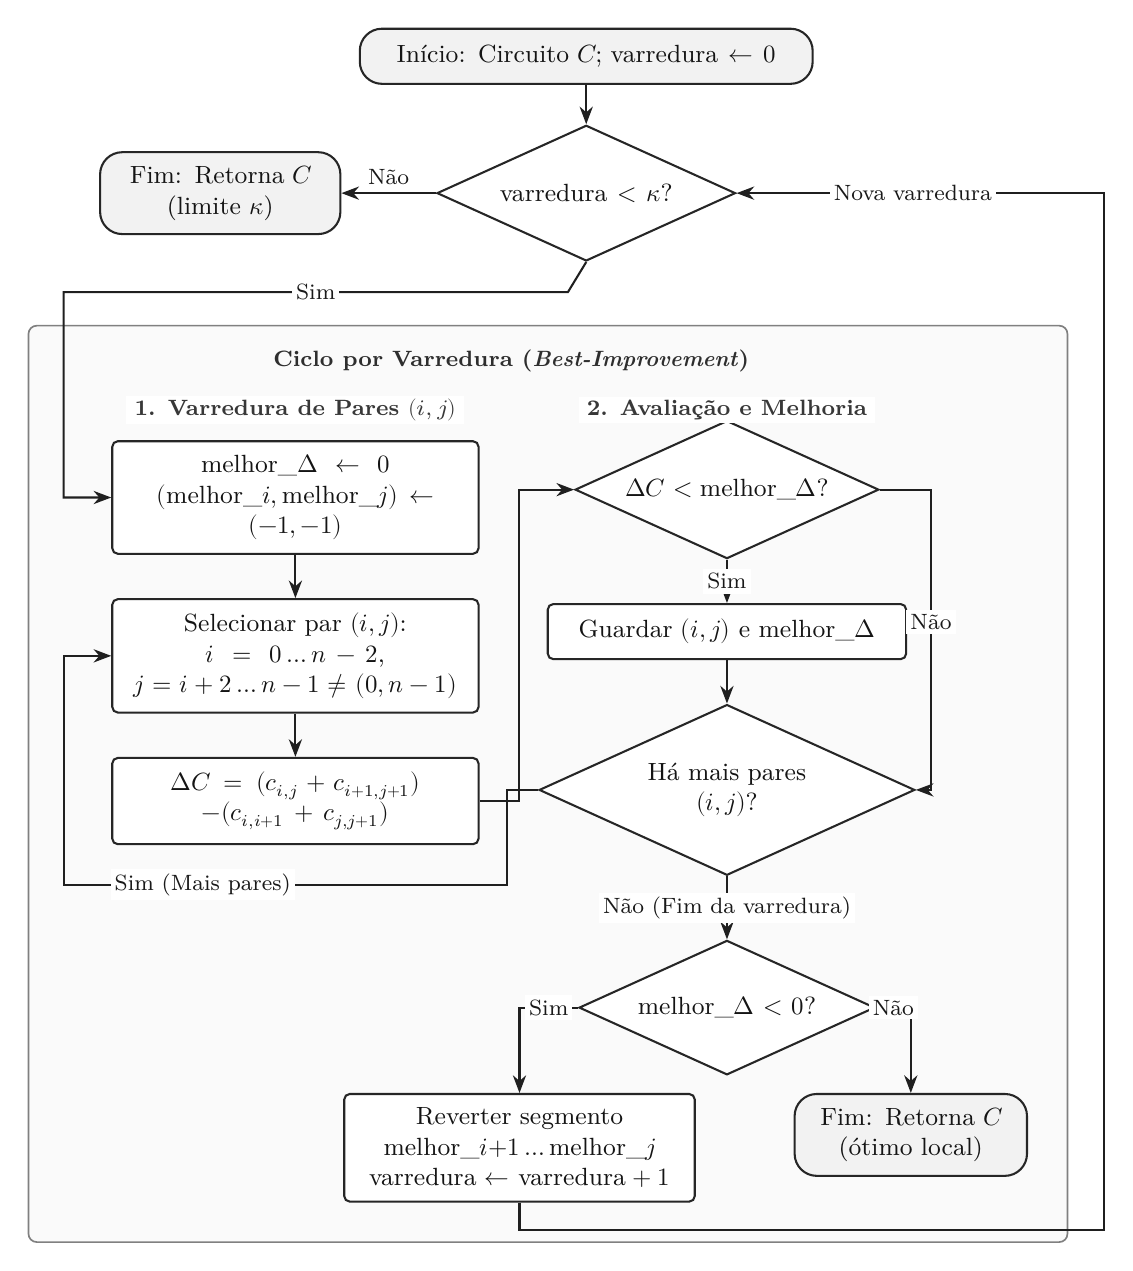
\begin{tikzpicture}[node distance=5mm and 8mm]
            % Topo (fora das colunas): Inicio e decisão de limite de varreduras
            \node[fc_term, text width=5.4cm] (start) {Início: Circuito \(C\); \(\text{varredura} \gets 0\)};
            \node[fc_dec, below=5mm of start, text width=2.7cm] (citer) {\(\text{varredura} < \kappa\)?};
            \node[fc_term, left=12mm of citer, text width=2.7cm] (endk) {Fim: Retorna \(C\)\\(limite \(\kappa\))};

            % Grupo externo: Ciclo por Varredura (Best-Improvement)
            % Subcoluna 1: 1. Varredura de Pares (i, j)
            \node[fc_proc, below left=27mm and 0.4cm of citer, text width=4.3cm] (reset) {\(\text{melhor\_}\Delta \gets 0\)\\\((\text{melhor\_}i, \text{melhor\_}j) \gets (-1, -1)\)};
            \node[fc_proc, below=5.5mm of reset, text width=4.3cm] (loops) {Selecionar par \((i, j)\):\\\(i = 0 \dots n-2\),\\\(j = i+2 \dots n-1 \neq (0, n-1)\)};
            \node[fc_proc, below=5.5mm of loops, text width=4.3cm] (calcd) {\(\Delta C = (c_{i,j} + c_{i+1,j+1})\)\\\(- (c_{i,i+1} + c_{j,j+1})\)};
            \node[fc_subgrouptitle, above=2mm of reset] (ts1) {1. Varredura de Pares \((i, j)\)};

            % Subcoluna 2: 2. Avaliação e Melhoria
            \node[fc_dec, right=12mm of reset, yshift=1mm, text width=2.7cm] (cdelta) {\(\Delta C < \text{melhor\_}\Delta\)?};
            \node[fc_proc, below=5.5mm of cdelta, text width=4.2cm] (store) {Guardar \((i, j)\) e \(\text{melhor\_}\Delta\)};
            \node[fc_dec, below=5.5mm of store, text width=2.7cm] (morep) {Há mais pares\\\((i, j)\)?};
            \node[fc_dec, below=8mm of morep, text width=2.6cm] (applyb) {\(\text{melhor\_}\Delta < 0\)?};
            \node[fc_proc, below left=6.5mm and -0.55cm of applyb, text width=4.1cm] (apply) {Reverter segmento\\\(\text{melhor\_}i{+}1 \dots \text{melhor\_}j\)\\\(\text{varredura} \gets \text{varredura} + 1\)};
            \node[fc_term, below right=6.5mm and -0.1cm of applyb, text width=2.6cm] (endopt) {Fim: Retorna \(C\)\\(ótimo local)};
            \node[fc_subgrouptitle] (ts2) at (ts1 -| cdelta) {2. Avaliação e Melhoria};

            % Titulo do grupo externo acima das subcolunas
            \node[fc_grouptitle, above=2.5mm of $(ts1.north)!0.5!(ts2.north)$] (touter) {Ciclo por Varredura (\emph{Best-Improvement})};

            % Caixas de fundo: subcolunas + grupo externo (margem esquerda para Sim e Mais pares)
            \begin{scope}[on background layer]
                  \node[fc_subgroup, fit=(ts1)(reset)(loops)(calcd)] (sg1) {};
                  \node[fc_subgroup, fit=(ts2)(cdelta)(store)(morep)(applyb)(apply)(endopt), inner sep=7pt] (sg2) {};
                  \coordinate (g1lpad) at ($(sg1.west)+(-5.5mm,0)$);
                  \node[fc_group, fit=(touter)(sg1)(sg2)(g1lpad), inner sep=7pt] (gouter) {};
            \end{scope}

            % Redesenha os títulos por cima do fundo
            \node[fc_subgrouptitle] at (ts1) {1. Varredura de Pares \((i, j)\)};
            \node[fc_subgrouptitle] at (ts2) {2. Avaliação e Melhoria};
            \node[fc_grouptitle] at (touter) {Ciclo por Varredura (\emph{Best-Improvement})};

            % Arestas topo (Sim contorna touter e ts1 pela esquerda entrando exatamente em reset.west)
            \coordinate (lchan) at ($(sg1.west)+(-3.5mm,0)$);
            \draw[fc_arr] (start) -- (citer);
            \draw[fc_arr] (citer.west) -- node[fc_lbl, above=1pt] {Não} (endk.east);
            \draw[fc_arr] (citer.south) -- ($(citer.south)!0.48!(gouter.north)$) -| node[fc_lbl, pos=0.25] {Sim} (lchan |- reset.west) -- (reset.west);

            % Fluxo dentro de Subcoluna 1
            \draw[fc_arr] (reset) -- (loops);
            \draw[fc_arr] (loops) -- (calcd);

            % Transição Subcoluna 1 -> Subcoluna 2 (entra pelo lado esquerdo de cdelta)
            \draw[fc_arr] (calcd.east) -- ++(5mm,0) |- (cdelta.west);

            % Fluxo dentro de Subcoluna 2
            \draw[fc_arr] (cdelta) -- node[fc_lbl] {Sim} (store);
            \draw[fc_arr] (store) -- (morep);
            \draw[fc_arr] (cdelta.east) -- ++(6.5mm,0) |- node[fc_lbl, pos=0.22] {Não} (morep.east);

            % Retorno interno: Mais pares volta EXATAMENTE para loops.west
            \draw[fc_arr] (morep.west) -- ++(-4mm,0) |- ($(calcd.south)+(0,-5mm)$) -| node[fc_lbl, pos=0.20] {Sim (Mais pares)} (lchan |- loops.west) -- (loops.west);

            % Fim da varredura -> Melhoria
            \draw[fc_arr] (morep.south) -- node[fc_lbl] {Não (Fim da varredura)} (applyb.north);
            \draw[fc_arr] (applyb.west) -| node[fc_lbl, pos=0.25] {Sim} (apply.north);
            \draw[fc_arr] (applyb.east) -| node[fc_lbl, pos=0.25] {Não} (endopt.north);

            % Canal externo direito limpo de retorno para varredura < kappa?
            \draw[fc_arr] (apply.south) -- ++(0,-3.5mm) -| ($(gouter.east)+(4.5mm,0)$) |- node[fc_lbl, pos=0.76] {Nova varredura} (citer.east);
      \end{tikzpicture}
      \caption{Fluxograma do algoritmo \(2\)-opt.}\label{fig:2opt-flowchart}
\end{figure}

O algoritmo \(2\)-opt limitado pode ser descrito formalmente pelo pseudocódigo apresentado no \algref{alg:2opt-limited} (\apref{apendice-pseudocodigos}).\footnote{Na implementação experimental avaliada neste trabalho, o laço interno restringe-se à tabela pré-computada de \(k_{\text{viz}} = \kviz\) vizinhos mais próximos de cada cidade, utilizando avaliação vetorizada em NumPy na linha de base em CPU e execução paralela por \emph{threads} e \emph{warps} nas variantes em GPU, conforme detalhado no \capref{cap3-materiais-metodos}.}

\section{Algoritmos genéticos}\label{sec-23-algoritmos-geneticos}

Algoritmos Genéticos (AGs, do inglês \emph{Genetic Algorithms} -- GAs) são meta-heurísticas inspiradas em princípios de evolução biológica, nas quais uma população de soluções candidatas é iterativamente modificada por operadores análogos à seleção natural, recombinação e mutação \autocite{goldberg1989genetic,eiben2015introduction}.
Em sua forma canônica, um AG mantém uma população \(P(t) = \{x_1^{(t)}, x_2^{(t)}, \dots, x_{n_{pop}}^{(t)}\}\) de \(n_{pop}\) indivíduos na geração \(t\); a cada geração, cada indivíduo \(x_i\) tem sua qualidade avaliada por uma função de aptidão (\emph{fitness}) \(f(x_i)\) --- que, no TSP, associa-se inversamente ao custo do circuito representado pela permutação ---, passando então por seleção, cruzamento e mutação até que um critério de parada seja atingido.

Embora AGs puros tendam a convergir mais lentamente do que heurísticas especializadas de busca local quando aplicados isoladamente ao TSP, eles oferecem quatro vantagens metodológicas decisivas para este estudo:
(i) \textbf{exploração global simultânea} de espaços de busca multimodais por meio da diversidade populacional, reduzindo a suscetibilidade à estagnação prematura em ótimos locais de baixa qualidade;
(ii) \textbf{recombinação de sub-rotas promissoras} (\emph{building blocks}) por meio de operadores de cruzamento especializados para permutações \autocite{goldberg1989genetic,larranaga1999genetic};
(iii) \textbf{paralelismo intrínseco em nível de dados} ao longo dos \(n_{pop}\) indivíduos, mapeando-se naturalmente para execução vetorial e SIMD/SIMT em GPUs; e
(iv) \textbf{modularidade para hibridização} com procedimentos de intensificação local.
Além disso, essa escolha acompanha a proposta interdisciplinar deste trabalho de integrar princípios de computação evolutiva, otimização combinatória e programação paralela massiva em GPU.

No contexto do TSP, cada solução é representada como uma permutação válida das cidades, utilizando operadores de recombinação e mutação que preservam a viabilidade da rota \autocite{larranaga1999genetic}.
O fluxo em alto nível e o ciclo detalhado com operadores específicos estão formalizados, respectivamente, no \algref{alg:ga-high-level} e no \algref{alg:ga-complete} (\apref{apendice-pseudocodigos}).
A \figref{fig:ga-flowchart} ilustra o fluxo geral desse processo iterativo \autocite{goldberg1989genetic,eiben2015introduction}.

\subsection{Operadores evolutivos e substituição populacional}\label{sec-231-operadores-substituicao}

A dinâmica evolutiva de um AG para problemas baseados em permutações depende da escolha coordenada de quatro componentes principais \autocite{goldberg1989genetic,eiben2015introduction,larranaga1999genetic}:

\begin{itemize}
      \item
            \textbf{Seleção de pais:} Escolhe indivíduos de \(P(t)\) para reprodução privilegiando soluções de melhor aptidão. Na seleção proporcional (roleta), definida pela Equação~\eqref{eq:selecao-proporcional}, a probabilidade de escolher o indivíduo \(x_i\) é proporcional à sua aptidão relativa na população (o que exige conversão adequada em problemas de minimização, como a inversão do custo):
            \begin{equation}\label{eq:selecao-proporcional}
                  p_i = \frac{f(x_i)}{\sum_{j=1}^{n_{pop}} f(x_j)}
            \end{equation}
            Como alternativa, a \textbf{seleção por torneio} de tamanho \(\tau_{\text{trnmt}}\) sorteia aleatoriamente \(\tau_{\text{trnmt}}\) indivíduos de \(P(t)\) e escolhe o de menor custo de rota. Este trabalho adota a seleção por torneio por dispensar reescalonamento global da aptidão e permitir execuções independentes e diretamente paralelizáveis em GPU \autocite{goldberg1989genetic,eiben2015introduction}.
      \item
            \textbf{Cruzamento (recombinação) em permutações:} Combina pares de progenitores, com probabilidade dada pela taxa de cruzamento \(p_c\), para gerar descendentes válidos. Como o corte simples de vetores gera repetições ou omissões de cidades, utilizam-se operadores especializados como o \emph{Partially Mapped Crossover} (PMX) e o \emph{Order Crossover} (OX) \autocite{larranaga1999genetic}. Adota-se neste trabalho o operador OX, que copia um segmento contíguo de um dos pais e preenche as posições restantes preservando a ordem relativa das cidades no outro progenitor.
      \item
            \textbf{Mutação:} Introduz perturbações estocásticas com taxa de mutação \(p_{\text{mut}}\) para manter a diversidade genética e evitar convergência prematura. Em rotas representadas por permutações, destacam-se a mutação por inversão de segmento e a \textbf{mutação por troca} (\emph{swap mutation}), adotada neste trabalho, na qual duas posições da permutação são sorteadas e trocadas entre si \autocite{larranaga1999genetic,eiben2015introduction}.
      \item
            \textbf{Seleção de sobreviventes (substituição populacional) e elitismo:} Define como a nova população \(P(t+1)\) é formada a partir de \(P(t)\) e dos descendentes. Na \textbf{substituição geracional}, o conjunto completo de descendentes substitui integralmente a população de pais a cada geração; em esquemas de \textbf{estado estacionário (\emph{steady-state})}, apenas uma pequena fração da população (frequentemente um ou dois indivíduos) é substituída por passo \autocite{eiben2015introduction}. Para evitar a perda estocástica das melhores soluções já descobertas, aplica-se o \textbf{elitismo}, que copia deterministicamente o(s) melhor(es) indivíduo(s) de \(P(t)\) para \(P(t+1)\), garantindo que a melhor rota encontrada seja mantida de forma monotônica ao longo das gerações \autocite{goldberg1989genetic,eiben2015introduction}.
\end{itemize}

\begin{figure}[htbp]
      \centering
      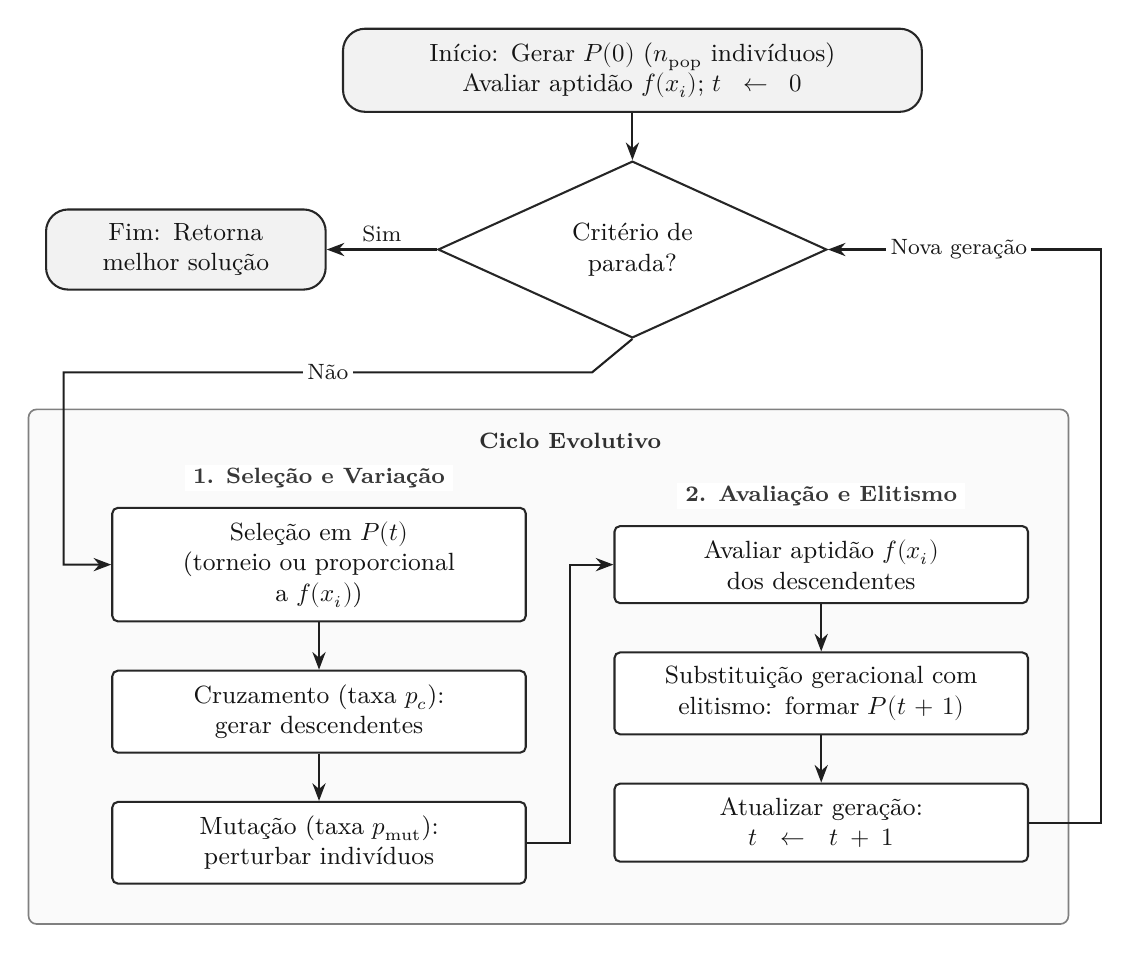
\begin{tikzpicture}[node distance=6mm and 10mm]
            % Topo centralizado (fora do ciclo)
            \node[fc_term, text width=7.0cm] (start) {Início: Gerar \(P(0)\) (\(n_{\text{pop}}\) indivíduos)\\Avaliar aptidão \(f(x_i)\); \(t \gets 0\)};
            \node[fc_dec, below=6mm of start, text width=2.9cm] (stop) {Critério de\\parada?};
            \node[fc_term, left=14mm of stop, text width=3.2cm] (out) {Fim: Retorna\\melhor solução};

            % Grupo externo: Ciclo Evolutivo (duas subcolunas equilibradas lado a lado)
            % Subcoluna 1: 1. Seleção e Variação
            \node[fc_proc, below left=27mm and 0.1cm of stop, text width=4.9cm] (sel) {Seleção em \(P(t)\)\\(torneio ou proporcional\\a \(f(x_i)\))};
            \node[fc_proc, below=6mm of sel, text width=4.9cm] (cross) {Cruzamento (taxa \(p_c\)):\\gerar descendentes};
            \node[fc_proc, below=6mm of cross, text width=4.9cm] (mut) {Mutação (taxa \(p_{\text{mut}}\)):\\perturbar indivíduos};
            \node[fc_subgrouptitle, above=2mm of sel] (ts1) {1. Seleção e Variação};

            % Subcoluna 2: 2. Avaliação e Elitismo
            \node[fc_proc, right=11mm of sel, text width=4.9cm] (evaln) {Avaliar aptidão \(f(x_i)\)\\dos descendentes};
            \node[fc_proc, below=6mm of evaln, text width=4.9cm] (repl) {Substituição geracional com\\elitismo: formar \(P(t+1)\)};
            \node[fc_proc, below=6mm of repl, text width=4.9cm] (inct) {Atualizar geração:\\\(t \gets t + 1\)};
            \node[fc_subgrouptitle, above=2mm of evaln] (ts2) {2. Avaliação e Elitismo};

            \node[fc_grouptitle, above=2.5mm of $(ts1.north)!0.5!(ts2.north)$] (touter) {Ciclo Evolutivo};

            % Caixas de fundo (margem esquerda para entrada Não sem cruzar títulos)
            \begin{scope}[on background layer]
                  \node[fc_subgroup, fit=(ts1)(sel)(cross)(mut)] (sg1) {};
                  \node[fc_subgroup, fit=(ts2)(evaln)(repl)(inct)] (sg2) {};
                  \coordinate (g2lpad) at ($(sg1.west)+(-5.5mm,0)$);
                  \node[fc_group, fit=(touter)(sg1)(sg2)(g2lpad), inner sep=7pt] (gouter) {};
            \end{scope}

            % Redesenha títulos por cima do fundo
            \node[fc_subgrouptitle] at (ts1) {1. Seleção e Variação};
            \node[fc_subgrouptitle] at (ts2) {2. Avaliação e Elitismo};
            \node[fc_grouptitle] at (touter) {Ciclo Evolutivo};

            % Arestas topo e entrada no ciclo (contorna touter e ts1 pela esquerda entrando exatamente em sel.west)
            \coordinate (lchan) at ($(sg1.west)+(-3.5mm,0)$);
            \coordinate (rchan) at ($(gouter.east)+(4mm,0)$);
            \draw[fc_arr] (start) -- (stop);
            \draw[fc_arr] (stop.west) -- node[fc_lbl, above=1pt] {Sim} (out.east);
            \draw[fc_arr] (stop.south) -- ($(stop.south)!0.48!(gouter.north)$) -| node[fc_lbl, pos=0.25] {Não} (lchan |- sel.west) -- (sel.west);

            % Fluxo interno das subcolunas e transição limpa entre elas
            \draw[fc_arr] (sel) -- (cross);
            \draw[fc_arr] (cross) -- (mut);
            \draw[fc_arr] (mut.east) -- ++(5.5mm,0) |- (evaln.west);
            \draw[fc_arr] (evaln) -- (repl);
            \draw[fc_arr] (repl) -- (inct);

            % Retorno limpo pelo canal externo direito
            \draw[fc_arr] (inct.east) -- (rchan |- inct.east) |- node[fc_lbl, pos=0.76] {Nova geração} (stop.east);
      \end{tikzpicture}
      \caption{Fluxograma de Algoritmo Genético.}\label{fig:ga-flowchart}
\end{figure}

\section{Meta-heurísticas híbridas}\label{sec-24-metaheuristicas-hibridas}

Em termos gerais, meta-heurísticas híbridas combinam duas ou mais estratégias de busca para aproveitar a complementaridade entre métodos com pontos fortes distintos.
No contexto de problemas de roteamento e, em particular, do TSP, é comum combinar heurísticas de construção (como vizinho mais próximo, inserções ou heurísticas baseadas em MST) com heurísticas de melhoria (como movimentos \(k\)-opt) ou com meta-heurísticas populacionais (como AGs), para que um componente forneça boas soluções iniciais ou exploração global enquanto o outro aprofunda a busca em vizinhanças \autocite{voudouris1999tsp}.

\textcite{crainic2003parallel,alba2005parallel,larranaga1999genetic} classificam abordagens híbridas e cooperativas em três categorias principais:
\begin{enumerate}[label=(\roman*)]
      \item
            \textbf{hibridização em nível de solução}, na qual uma meta-heurística incorpora sistematicamente um procedimento de busca local para refinar soluções candidatas individuais;
      \item
            \textbf{hibridização em nível de algoritmo}, em que diferentes técnicas (por exemplo, um método exato e uma meta-heurística, ou múltiplas buscas simultâneas) são combinadas em arquiteturas integradas ou esquemas cooperativos; e
      \item
            \textbf{hibridizações multiestágio}, nas quais diferentes métodos atuam sequencialmente em fases distintas do processo de resolução (inicialização construtiva, intensificação local e diversificação).
\end{enumerate}
Essa classificação ajuda a organizar a variedade de abordagens híbridas descritas na literatura, embora nem sempre existam fronteiras rígidas entre as categorias.

Uma extensão consolidada dessa ideia são os algoritmos meméticos, nos quais operadores evolutivos (seleção, cruzamento e mutação) são acoplados sistematicamente a heurísticas de busca local aplicadas aos indivíduos da população \autocite{larranaga1999genetic}.
Em problemas de roteamento, isso resulta em esquemas AG+LS, nos quais um AG conduz a exploração global do espaço de soluções e um procedimento de melhoria, como \(2\)-opt ou Lin--Kernighan, refina soluções promissoras.
Esses algoritmos oferecem melhor equilíbrio entre diversificação e intensificação do que AGs puros, ao custo de maior esforço computacional por geração.
Trabalhos como o de \textcite{fujimoto2011highly} exploram justamente essa combinação AG+busca local para o TSP em ambientes paralelos, motivando a arquitetura investigada neste estudo.

\section{Algoritmos meméticos}\label{sec-25-algoritmos-memeticos}

Algoritmos meméticos constituem uma família de meta-heurísticas evolutivas que incorporam explicitamente operadores de busca local ao ciclo de evolução populacional \autocite{larranaga1999genetic}.
A metáfora usual associa o termo ``meme'' a unidades de informação que se propagam e se aperfeiçoam ao longo das gerações: além da recombinação e mutação de indivíduos, há uma etapa de intensificação local sobre cada solução, promovendo seu refinamento iterativo.

Em um algoritmo memético típico, a cada geração, indivíduos selecionados (ou toda a população de descendentes) são submetidos a um procedimento de busca local, como \(2\)-opt, \(3\)-opt ou Lin--Kernighan no caso do TSP.
Esse acoplamento permite conduzir soluções já competitivas até ótimos locais de alta qualidade, enquanto o AG mantém a diversidade global por meio da seleção, do cruzamento e da mutação.

O projeto de um algoritmo memético envolve três decisões arquiteturais distintas \autocite{larranaga1999genetic}:
\begin{enumerate}[label=(\roman*)]
      \item
            \textbf{Alcance populacional:} quais indivíduos recebem busca local (apenas a elite, um subconjunto amostrado ou todos os descendentes gerados);
      \item
            \textbf{Periodicidade e estágio de acoplamento:} em que momento do ciclo geracional a intensificação local é acionada (por exemplo, após a inicialização, após a mutação ou apenas a cada intervalo fixo de gerações); e
      \item
            \textbf{Profundidade de refinamento:} o orçamento máximo de varreduras \(\kappa\) permitido por chamada da busca local sobre cada indivíduo.
\end{enumerate}
Essas escolhas determinam diretamente o equilíbrio entre qualidade das soluções, custo computacional e preservação da diversidade populacional.

Estudos fundamentais, como o de \textcite{larranaga1999genetic}, indicam que algoritmos meméticos apresentam desempenho expressivo para o TSP quando combinam operadores de cruzamento específicos para rotas com busca local intensiva.
A viabilidade de acelerar esse paradigma em GPU foi reforçada por \textcite{fujimoto2011highly}, que implementaram um AG memético em uma GPU NVIDIA GTX285 com reduções paralelas para gerenciar a avaliação e a busca local.
Em comparação com uma execução sequencial em processador de um único núcleo (\emph{single-core}), observaram aceleração de até \(24{,}2\times\) na instância \texttt{ts225}, mostrando que mesmo instâncias de porte médio já se beneficiam expressivamente do paralelismo em GPU.

\subsection{Algoritmo Genético Hibridizado com \texorpdfstring{\(2\)-opt}{2-opt}}\label{sec-251-ga-2opt}

O esquema AG+\(2\)-opt adotado neste trabalho segue a estrutura clássica de algoritmos meméticos geracionais para o TSP \autocite{larranaga1999genetic}, usando representação por permutação de inteiros e combinando operadores evolutivos padronizados com uma busca local \(2\)-opt truncada.
Em cada geração \(t\), o fluxo completo do algoritmo é composto por sete etapas sequenciais:

\begin{enumerate}
      \item
            \textbf{Inicialização (\(t=0\)):} Gerar a população inicial \(P(0)\) com \(n_{pop}\) permutações válidas das \(n_{coords}\) cidades (aleatoriamente ou por heurística construtiva).
      \item
            \textbf{Avaliação (\emph{fitness}):} Avaliar a aptidão \(f(x_i)\) de cada rota \(x_i \in P(t)\) a partir do custo total (comprimento) do circuito.
      \item
            \textbf{Seleção:} Escolher pares de progenitores em \(P(t)\) por seleção por torneio de tamanho \(\tau_{\text{trnmt}}\), favorecendo soluções de menor custo sem necessidade de reescalonamento global.
      \item
            \textbf{Cruzamento:} Recombinar pares de progenitores selecionados com taxa \(p_c\) via \emph{Order Crossover} (OX), gerando descendentes que preservam a validade da permutação e a ordem relativa das cidades herdadas.
      \item
            \textbf{Mutação:} Aplicar a mutação por troca (\emph{swap mutation}) com taxa \(p_{\text{mut}}\), trocando duas posições da rota para manter a diversidade genética.
      \item
            \textbf{Busca local \(2\)-opt truncada (\(\mathcal{L}(x, \kappa)\)):} Aplicar o operador de refinamento \(\mathcal{L}(x, \kappa)\) sobre cada descendente gerado após a mutação. Cada chamada executa varreduras sucessivas sob o critério \emph{best-improvement} na vizinhança restrita pela lista estática de \(k_{\text{viz}} = \kviz\) vizinhos mais próximos: em cada varredura, todos os pares candidatos admissíveis são avaliados pela Equação~\eqref{eq:delta-2opt} e aplica-se no máximo \textbf{uma} reversão de segmento --- a de menor \(\Delta C < 0\). O refinamento de cada indivíduo encerra-se por critério duplo: ao atingir um ótimo local na vizinhança candidata (\(\Delta C \ge 0\)) ou ao completar o limite de \(\kappa = \maxpassadas\) varreduras completas (e não ``\(\maxpassadas\) nós'' ou ``\(\maxpassadas\) trocas'' arbitrárias), teto que limita o custo computacional por geração.
      \item
            \textbf{Substituição com elitismo:} Formar \(P(t+1)\) preservando deterministicamente o(s) melhor(es) indivíduo(s) de \(P(t)\) e preenchendo as demais vagas com os descendentes refinados.
\end{enumerate}

\begin{quote}
      \textbf{Exemplo ilustrativo.} Considere uma rota \(C = (v_0, v_1, v_2, v_3, v_4, v_5)\) com \(n_{coords} = 6\) cidades e orçamento máximo \(\kappa = \maxpassadas\).
      Em uma única varredura \emph{best-improvement} exaustiva sob \(0 \le i < 5\), \(i+2 \le j < 6\) e \((i,j) \neq (0,5)\), avaliam-se os \(n_{coords}(n_{coords}-3)/2 = 9\) pares admissíveis: \((0,2)\), \((0,3)\), \((0,4)\), \((1,3)\), \((1,4)\), \((1,5)\), \((2,4)\), \((2,5)\) e \((3,5)\).
      Suponha que, na primeira varredura, o par de menor \(\Delta C < 0\) seja \((i,j) = (1,4)\); o segmento \((v_2, v_3, v_4)\) é invertido uma vez.
      Na segunda varredura, a busca reavalia o circuito já modificado, no qual novas arestas foram criadas após a reversão.
      Caso na terceira varredura não exista nenhum par com \(\Delta C < 0\), o procedimento \(\mathcal{L}(x, \maxpassadas)\) é encerrado antecipadamente antes de atingir o teto \(\kappa = \maxpassadas\).
\end{quote}

O ciclo geracional repete-se até que um critério de parada seja atendido (alcance do ótimo conhecido dentro da tolerância, estagnação da melhor solução ou limite máximo de gerações).
A \figref{fig:ga2opt-flowchart} ilustra o fluxo completo do algoritmo AG+\(2\)-opt memético \autocite{larranaga1999genetic}, destacando a inserção da busca local \(\mathcal{L}(x, \kappa)\) após os operadores genéticos e antes da substituição populacional.

\begin{figure}[htbp]
      \centering
      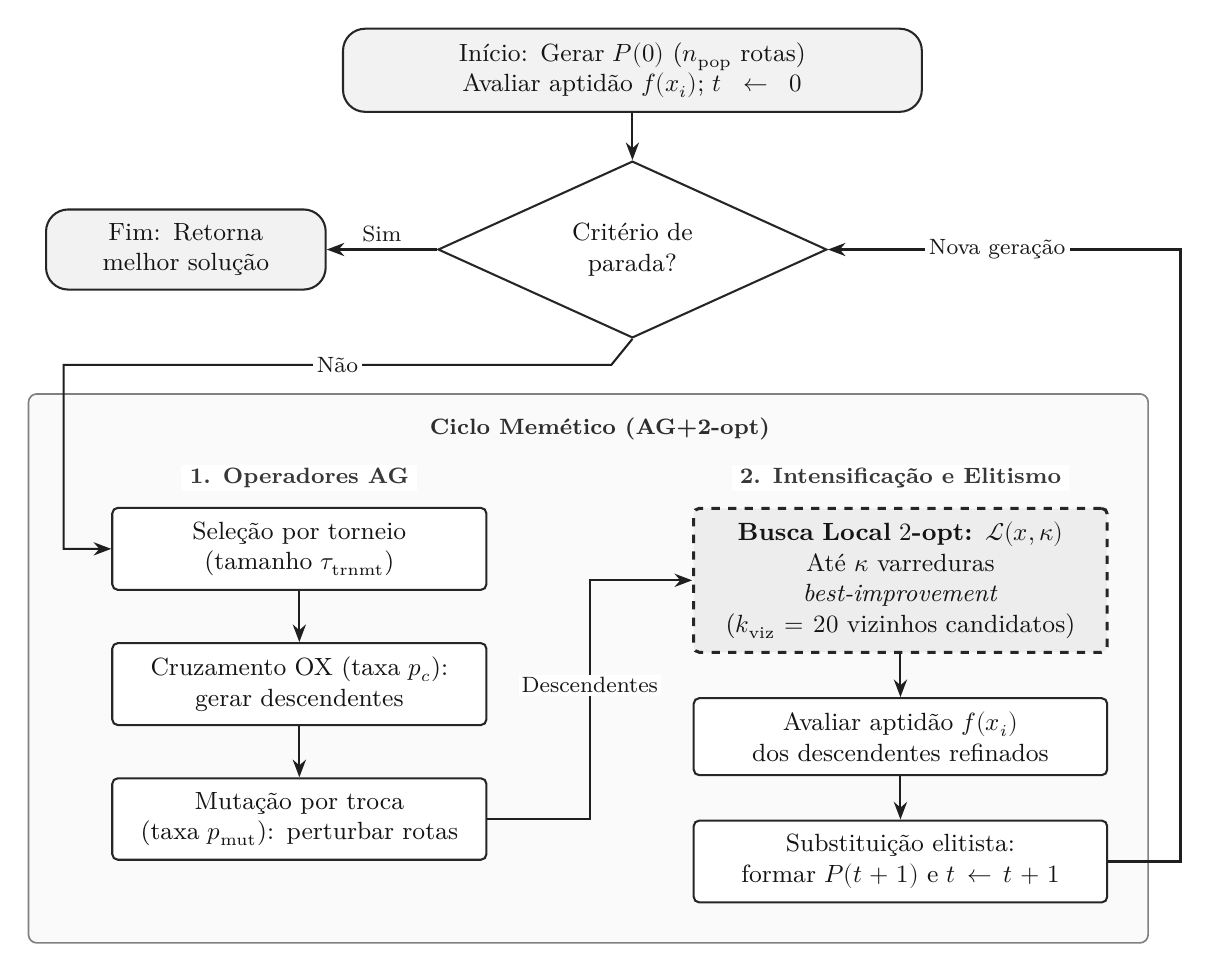
\begin{tikzpicture}[node distance=6mm and 10mm]
            % Topo centralizado (fora do ciclo)
            \node[fc_term, text width=7.0cm] (start) {Início: Gerar \(P(0)\) (\(n_{\text{pop}}\) rotas)\\Avaliar aptidão \(f(x_i)\); \(t \gets 0\)};
            \node[fc_dec, below=6mm of start, text width=2.9cm] (stop) {Critério de\\parada?};
            \node[fc_term, left=14mm of stop, text width=3.2cm] (out) {Fim: Retorna\\melhor solução};

            % Grupo externo: Ciclo Memético (AG+2-opt) com 2 subcolunas de mesma altura
            % Subcoluna 1: 1. Operadores AG
            \node[fc_proc, below left=27mm and 0.6cm of stop, text width=4.4cm] (sel) {Seleção por torneio\\(tamanho \(\tau_{\text{trnmt}}\))};
            \node[fc_proc, below=6.5mm of sel, text width=4.4cm] (cross) {Cruzamento OX (taxa \(p_c\)):\\gerar descendentes};
            \node[fc_proc, below=6.5mm of cross, text width=4.4cm] (mut) {Mutação por troca\\(taxa \(p_{\text{mut}}\)): perturbar rotas};
            \node[fc_subgrouptitle, above=2mm of sel] (ts1) {1. Operadores AG};

            % Subcoluna 2: 2. Intensificação e Elitismo (alinhado pelo topo com sel para Não empurrar touter)
            \node[fc_memetic, right=26mm of sel.north east, anchor=north west, text width=4.9cm] (ls) {\textbf{Busca Local \(2\)-opt:} \(\mathcal{L}(x, \kappa)\)\\Até \(\kappa\) varreduras \emph{best-improvement}\\(\(k_{\text{viz}} = \kviz\) vizinhos candidatos)};
            \node[fc_proc, below=5.5mm of ls, text width=4.9cm] (evaln) {Avaliar aptidão \(f(x_i)\)\\dos descendentes refinados};
            \node[fc_proc, below=5.5mm of evaln, text width=4.9cm] (repl) {Substituição elitista:\\formar \(P(t+1)\) e \(t \gets t + 1\)};
            \node[fc_subgrouptitle, above=2mm of ls] (ts2) {2. Intensificação e Elitismo};

            \node[fc_grouptitle, above=2.5mm of $(ts1.north)!0.5!(ts2.north)$] (touter) {Ciclo Memético (\(\text{AG+2-opt}\))};

            % Caixas de fundo (margem esquerda para entrada Não sem cruzar títulos)
            \begin{scope}[on background layer]
                  \node[fc_subgroup, fit=(ts1)(sel)(cross)(mut)] (sg1) {};
                  \node[fc_subgroup, fit=(ts2)(ls)(evaln)(repl)] (sg2) {};
                  \coordinate (g3lpad) at ($(sg1.west)+(-5.5mm,0)$);
                  \node[fc_group, fit=(touter)(sg1)(sg2)(g3lpad), inner sep=7pt] (gouter) {};
            \end{scope}

            % Redesenha títulos por cima do fundo
            \node[fc_subgrouptitle] at (ts1) {1. Operadores AG};
            \node[fc_subgrouptitle] at (ts2) {2. Intensificação e Elitismo};
            \node[fc_grouptitle] at (touter) {Ciclo Memético (\(\text{AG+2-opt}\))};

            % Arestas topo e entrada no ciclo (contorna touter e ts1 pela esquerda entrando exatamente em sel.west)
            \coordinate (lchan) at ($(sg1.west)+(-3.5mm,0)$);
            \coordinate (rchan) at ($(gouter.east)+(4mm,0)$);
            \draw[fc_arr] (start) -- (stop);
            \draw[fc_arr] (stop.west) -- node[fc_lbl, above=1pt] {Sim} (out.east);
            \draw[fc_arr] (stop.south) -- ($(stop.south)!0.48!(gouter.north)$) -| node[fc_lbl, pos=0.25] {Não} (lchan |- sel.west) -- (sel.west);

            % Fluxo interno e transição Descendentes no vão entre subcolunas
            \draw[fc_arr] (sel) -- (cross);
            \draw[fc_arr] (cross) -- (mut);
            \draw[fc_arr] (mut.east) -- ++(13mm,0) |- node[fc_lbl, pos=0.28, inner sep=1pt] {Descendentes} (ls.west);
            \draw[fc_arr] (ls) -- (evaln);
            \draw[fc_arr] (evaln) -- (repl);

            % Retorno limpo pelo canal externo direito
            \draw[fc_arr] (repl.east) -- (rchan |- repl.east) |- node[fc_lbl, pos=0.76] {Nova geração} (stop.east);
      \end{tikzpicture}
      \caption{Fluxograma do algoritmo AG+\(2\)-opt.}\label{fig:ga2opt-flowchart}
\end{figure}

No contexto experimental desta monografia, esse esquema AG+\(2\)-opt é implementado de forma equivalente em quatro estratégias de execução (CPU, Híbrida Ingênua, Híbrida Otimizada e Totalmente em GPU), mantendo idênticos os operadores, a vizinhança de \(k_{\text{viz}} = \kviz\) candidatos, o critério \emph{best-improvement} e o teto \(\kappa = \maxpassadas\).
Os detalhes de parametrização (\(n_{pop}\), \(p_c\), \(p_{\text{mut}}\), \(\tau_{\text{trnmt}}\), \(\kappa\), \(k_{\text{viz}}\)) e os critérios de parada adotados são apresentados no \capref{cap3-materiais-metodos}.

\section{Computação em GPU e paralelização de meta-heurísticas}\label{sec-26-gpu-metaheuristicas}

Processadores gráficos (GPUs) evoluíram, nas últimas décadas, de dispositivos voltados à renderização gráfica para plataformas de computação de uso geral (GPGPU --- \emph{General-Purpose Computing on GPUs}), amplamente utilizadas em computação científica, otimização e inteligência artificial \autocite{nvidia2024cuda}.
Em linhas gerais, o modelo de execução que agrupa dezenas de \emph{threads} em unidades de passo coordenado (\emph{lockstep}) no hardware é uma característica fundamental das arquiteturas modernas de GPU: em plataformas NVIDIA CUDA, esse paradigma é denominado SIMT (\emph{Single Instruction, Multiple Threads}) e as unidades de execução correspondem a \emph{warps} de \(32\) \emph{threads} \autocite{nvidia2024cuda}, de forma análoga aos \emph{wavefronts} adotados em arquiteturas AMD (ROCm/GCN/RDNA).
Com raízes na classe SIMD da taxonomia de \textcite{flynn1972taxonomy}, o modelo SIMT combina eficiência vetorial no hardware com a abstração de programação por \emph{threads} organizadas em grades (\emph{grids}) de blocos, permitindo que milhares de \emph{threads} executem o mesmo \emph{kernel} sobre dados distintos.

Essa organização estabelece um contraste direto em relação às CPUs convencionais.
Enquanto a CPU opera predominantemente como uma arquitetura MIMD (\emph{Multiple Instruction, Multiple Data}) no nível de núcleos independentes --- ainda que explore extensões vetoriais SIMD, como SSE e AVX, dentro de cada núcleo \autocite{flynn1972taxonomy} --- e dedica grande parte do silício a lógica complexa de controle, previsão de desvios e múltiplos níveis de \emph{cache} para minimizar a latência de fluxos de instruções independentes, a GPU prioriza a vazão (\emph{throughput}).
Para isso, o hardware da GPU escalona grupos de \emph{threads} (\emph{warps} ou \emph{wavefronts}) em passo coordenado sempre que não há divergência de controle, sendo particularmente adequado a cargas em que a mesma sequência de operações recai sobre grandes volumes de dados independentes.

\subsection{Taxonomia de paralelização segundo Crainic e Toulouse}\label{sec-261-taxonomia-paralelizacao}

A taxonomia proposta por \textcite{crainic2003parallel} e aprofundada em \textcite{crainic2010parallel} classifica as estratégias de paralelização de meta-heurísticas em três categorias principais, cada uma com adequação distinta às arquiteturas de hardware:

\begin{enumerate}
      \item \textbf{Tipo 1: Paralelismo de Baixo Nível (Decomposição de Dados).}
            Essa estratégia paraleliza tarefas computacionalmente pesadas dentro de cada iteração da meta-heurística, como o cálculo da função objetivo ou a avaliação de movimentos em uma vizinhança, mantendo inalterado o fluxo de controle sequencial do algoritmo.
            É particularmente adequada a arquiteturas SIMD/SIMT (GPUs), pois a mesma operação (como o cálculo de variação de custo em rotas) é aplicada simultaneamente a grandes conjuntos de dados independentes, maximizando o \emph{throughput} e diluindo o \emph{overhead} de lançamento de \emph{kernels}.
            Na literatura do TSP, \textcite{tsp_gpu} aplicam o paralelismo Tipo~1 à busca local \(2\)-opt em GPU, atribuindo a avaliação de cada movimento candidato a uma \emph{thread} distinta para explorar vizinhanças amplas em tempo reduzido.

      \item \textbf{Tipo 2: Decomposição de Domínio (Particionamento do Espaço de Busca).}
            O espaço de busca ou as variáveis de decisão são particionados em subconjuntos menores, e instâncias da meta-heurística operam em paralelo sobre cada partição antes de recombinar resultados parciais.
            Essa abordagem ajusta-se melhor a arquiteturas MIMD (CPUs \emph{multicore} ou \emph{clusters} distribuídos), porque subproblemas distintos frequentemente exibem cargas assimétricas e tempos de convergência variados --- cenário que provocaria divergência de controle e subutilização dentro de \emph{warps} em GPU.
            Um exemplo clássico ocorre no Problema de Roteamento de Veículos com Múltiplos Depósitos (MDVRP) \autocites{crainic2010parallel}{simchi2005logic}, em que cada depósito é atribuído a um núcleo ou \emph{thread} independente de uma CPU \emph{multicore} (ou a um nó/processo próprio em um \emph{cluster} distribuído), comunicando-se apenas periodicamente para trocar clientes localizados nas fronteiras entre regiões.

      \item \textbf{Tipo 3: Múltiplas Trajetórias (Buscas Independentes ou Cooperativas).}
            Múltiplas execuções da mesma meta-heurística --- ou de meta-heurísticas heterogêneas --- exploram o espaço de soluções de forma simultânea, seja de forma independente (\emph{multi-start}), seja de forma cooperativa por meio da troca periódica de soluções.
            Trata-se de uma categoria versátil: adapta-se bem a CPUs e \emph{clusters} via \emph{multithreading} ou \emph{multiprocessing} quando as trajetórias são complexas e heterogêneas, mas também escala em GPUs quando diversas buscas leves e estruturalmente idênticas são executadas em paralelo, incluindo esquemas combinados com paralelismo Tipo~1 revisados por \textcite{schulz2013gpu}.
            Como exemplo em GPU, \textcite{luong2013gpu} implementam modelos de ilhas nos quais dezenas ou centenas de subpopulações evoluem em paralelo em blocos de \emph{threads} distintos, migrando periodicamente seus melhores indivíduos via memória compartilhada.
\end{enumerate}

A \tabref{tbl:crainic-taxonomy} sintetiza as características contrastantes desses três tipos, enquanto a \figref{fig:crainic-taxonomy} ilustra a ramificação conceitual a partir de uma meta-heurística sequencial.

\begin{table}[htbp]
      \centering
      \caption{Síntese comparativa da taxonomia de paralelização de Crainic e Toulouse}\label{tbl:crainic-taxonomy}
      \footnotesize
      \begin{tabular}{@{}
                  >{\raggedright\arraybackslash}p{(\linewidth - 8\tabcolsep) * \real{0.15}}
                  >{\raggedright\arraybackslash}p{(\linewidth - 8\tabcolsep) * \real{0.21}}
                  >{\raggedright\arraybackslash}p{(\linewidth - 8\tabcolsep) * \real{0.19}}
                  >{\raggedright\arraybackslash}p{(\linewidth - 8\tabcolsep) * \real{0.22}}
                  >{\raggedright\arraybackslash}p{(\linewidth - 8\tabcolsep) * \real{0.23}}@{}}
            \toprule
            Tipo                                                                              & Alvo da paralelização & Alteração na trajetória de busca & Adequação em CPU vs.\ GPU & Aplicação neste trabalho / Exemplo \\
            \midrule
            \textbf{Tipo 1} (Baixo nível)                                                     &
            Cálculos intensivos intra-iteração (vizinhança e aptidão)                         &
            Nenhuma; preserva a trajetória sequencial original                                &
            Alta adequação a \textbf{GPU (SIMT)} quando há alto volume de dados uniformes     &
            \textbf{Adotado neste trabalho:} \(2\)-opt e avaliação simultânea da matriz de rotas na GPU \autocite{tsp_gpu}                                                                                                \\
            \addlinespace[4pt]
            \textbf{Tipo 2} (Domínio)                                                         &
            Partições disjuntas do espaço de busca ou variáveis                               &
            Altera a busca ao resolver subproblemas acoplados                                 &
            Preferível em \textbf{CPU/cluster (MIMD)} por cargas e desvios assimétricos       &
            MDVRP com um núcleo/\emph{thread} por depósito e troca de fronteira \autocites{crainic2010parallel}{simchi2005logic}                                                                                          \\
            \addlinespace[4pt]
            \textbf{Tipo 3} (Múltiplas trajetórias)                                           &
            Execuções completas independentes ou cooperativas                                 &
            Explora múltiplas trajetórias simultâneas no espaço                               &
            \textbf{CPU/cluster} para buscas heterogêneas; \textbf{GPU} para ilhas homogêneas &
            Modelos de ilhas por bloco de \emph{threads} em GPU \autocites{luong2013gpu}{schulz2013gpu}                                                                                                                   \\
            \bottomrule
      \end{tabular}
\end{table}

\begin{figure}[htbp]
      \centering
      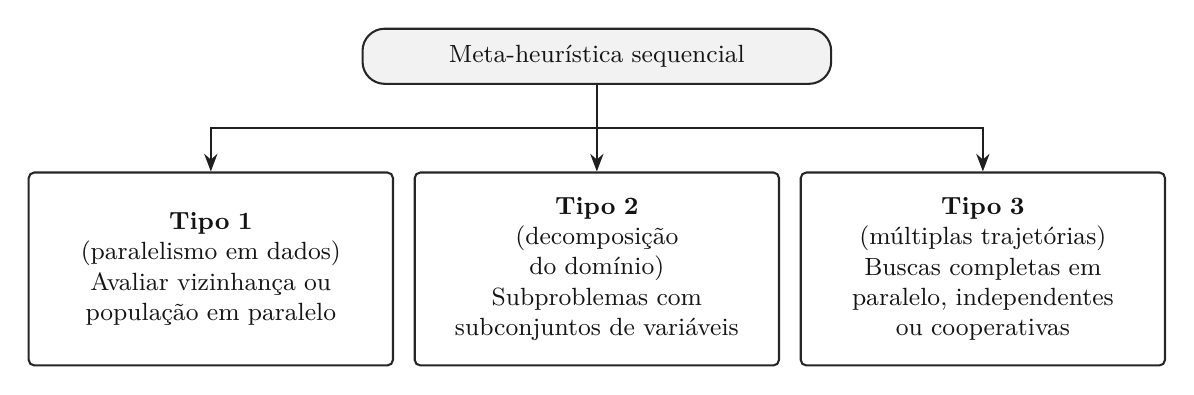
\begin{tikzpicture}[node distance=11mm and 2.5mm]
            \node[fc_term, text width=5.6cm] (mh) {Meta-heurística sequencial};
            \node[fc_proc, below=11mm of mh, text width=4.38cm, inner xsep=3.5pt, minimum height=2.45cm] (t2) {\textbf{Tipo 2}\\(decomposição\\do domínio)\\Subproblemas com\\subconjuntos de variáveis};
            \node[fc_proc, left=2.5mm of t2.north west, anchor=north east, text width=4.38cm, inner xsep=3.5pt, minimum height=2.45cm] (t1) {\textbf{Tipo 1}\\(paralelismo em dados)\\Avaliar vizinhança ou\\população em paralelo};
            \node[fc_proc, right=2.5mm of t2.north east, anchor=north west, text width=4.38cm, inner xsep=3.5pt, minimum height=2.45cm] (t3) {\textbf{Tipo 3}\\(múltiplas trajetórias)\\Buscas completas em\\paralelo, \mbox{independentes}\\ou cooperativas};

            \coordinate (branch) at ($(mh.south)+(0,-5.5mm)$);
            \draw[fc_arr] (mh.south) -- (t2.north);
            \draw[fc_arr] (mh.south) -- (branch) -| (t1.north);
            \draw[fc_arr] (mh.south) -- (branch) -| (t3.north);
      \end{tikzpicture}
      \caption{Resumo dos três tipos de paralelização de Crainic e Toulouse.}\label{fig:crainic-taxonomy}
\end{figure}

Neste trabalho, as variantes desenvolvidas enquadram-se principalmente no \textbf{Tipo 1}, concentrando o paralelismo em dados na avaliação de vizinhança \(2\)-opt e, na variante residente, também nos operadores genéticos e no cálculo de aptidão da população em GPU.

\subsection{Aplicações de GPU a meta-heurísticas para o TSP}\label{sec-262-gpu-aplicacoes-tsp}

Aplicações de GPU a meta-heurísticas para o TSP concentram-se principalmente no paralelismo em dados, tanto na avaliação paralela da aptidão de rotas em algoritmos genéticos (por meio de operações de redução) quanto na exploração simultânea de movimentos de vizinhança em heurísticas de melhoria local \autocite{schulz2013gpu,tsp_gpu,fujimoto2011highly}.
Outros trabalhos investigam a paralelização de Recozimento Simulado, Colônias de Formigas (ACO) e outras meta-heurísticas em GPU, geralmente aproveitando o grande número de \emph{threads} para explorar múltiplas soluções ou vizinhanças em cada passo da busca \autocite{binjubier2024gpu,rey2018cpu,abdelatti2020improvedgpuheuristic}.
Esses estudos motivam o uso de GPUs para acelerar algoritmos meméticos, mas também evidenciam desafios ligados à movimentação de dados entre CPU e GPU, à escolha de granularidade adequada de \emph{kernels}, à ocupação dos multiprocessadores e às limitações de memória (VRAM).
Esses aspectos são retomados no \capref{cap3-materiais-metodos}, que descreve o projeto dos \emph{kernels} de \(2\)-opt e as estratégias de gerenciamento de memória adotadas neste estudo.

\subsection{Contraste arquitetural: CPU vs GPU}\label{sec-263-cpu-vs-gpu}

As Figuras~\ref{fig:cpu-gpu-contrast},~\ref{fig:cpu-gpu-detail} e~\ref{fig:gpu-internal} ajudam a visualizar, de forma simples, como CPUs e GPUs foram projetadas para resolver problemas distintos.
De maneira geral, CPUs têm poucos núcleos mais complexos e flexíveis.
Uma parte grande da área do chip é usada para controle de fluxo, previsão de desvios e vários níveis de \emph{cache}, o que favorece programas sequenciais, com muitas decisões e acesso irregular à memória.
Nas GPUs acontece o contrário: a maior parte da área é ocupada por muitas unidades aritméticas simples (ALUs), organizadas em centenas ou milhares de núcleos em paralelo.
Elas abrem mão de um controle sofisticado para ganhar vazão (\emph{throughput}) quando muitas \emph{threads} executam a mesma sequência de instruções sobre dados diferentes.
Essa diferença explica por que GPUs funcionam bem para tarefas com muito paralelismo em dados, como avaliar muitas rotas de uma vez ou aplicar \(2\)-opt em vários indivíduos em paralelo.

\begin{figure}
      \centering
      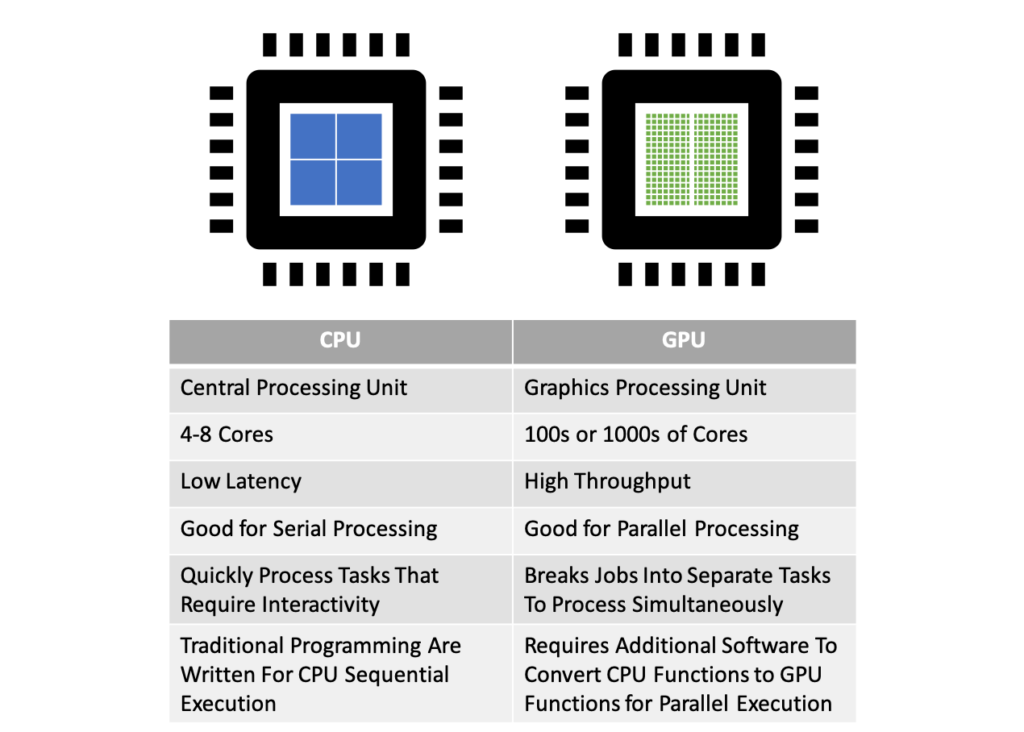
\includegraphics[width=0.8\linewidth,height=\textheight,keepaspectratio]{cpu-gpu-architecture-comparison.png}
      \caption{Comparação simplificada entre arquitetura de CPU e GPU. Fonte:
            \textcite{layerstack2023cpugpu}.}\label{fig:cpu-gpu-contrast}
\end{figure}

A \figref{fig:cpu-gpu-detail} mostra esse contraste na divisão da área do chip.
Em uma CPU típica, poucos núcleos complexos dividem espaço com grandes \emph{caches} e lógica de controle.
Em uma GPU, o projeto é o inverso: a maior parte da área é dedicada a conjuntos de núcleos de processamento paralelo (por exemplo, \emph{CUDA cores} em GPUs NVIDIA ou \emph{stream processors} em GPUs AMD) e à memória de alta largura de banda.
O controle é mais simples, mas o número de operações por segundo é muito maior quando o problema é bem mapeado para esse tipo de arquitetura \autocite{paz2011gpucpuimage}.

\begin{figure}
      \centering
      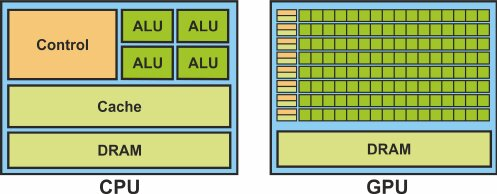
\includegraphics[width=0.8\linewidth,height=\textheight,keepaspectratio]{cpu-gpu-silicon-allocation.png}
      \caption{Alocação de silício em CPU e GPU. Adaptado de
            \textcite{paz2011gpucpuimage}.}\label{fig:cpu-gpu-detail}
\end{figure}

A \figref{fig:gpu-internal} resume como esses recursos aparecem na organização interna de uma GPU moderna.
A memória global (DRAM) oferece grande largura de banda, mas latência alta; cada \emph{streaming multiprocessor} (SM) possui memórias compartilhadas menores e registradores, usados pelas \emph{threads} de um mesmo bloco.
As \emph{threads} são agrupadas em \emph{warps} (de \(32\) \emph{threads} nas GPUs NVIDIA), que constituem a menor unidade indivisível de escalonamento e emissão de instruções no hardware: todas as \emph{threads} de um mesmo \emph{warp} recebem e executam simultaneamente a mesma instrução, embora cada uma opere sobre seus próprios registradores e dados distintos, seguindo o modelo SIMT \autocite{shah2023gpuarchitectureimage}.
Quando as \emph{threads} de um \emph{warp} seguem caminhos de controle diferentes ou acessam a memória de forma muito irregular, parte desse paralelismo é perdida; quando o acesso é organizado e o fluxo de controle é uniforme, o ganho de desempenho é expressivo.

\begin{figure}
      \centering
      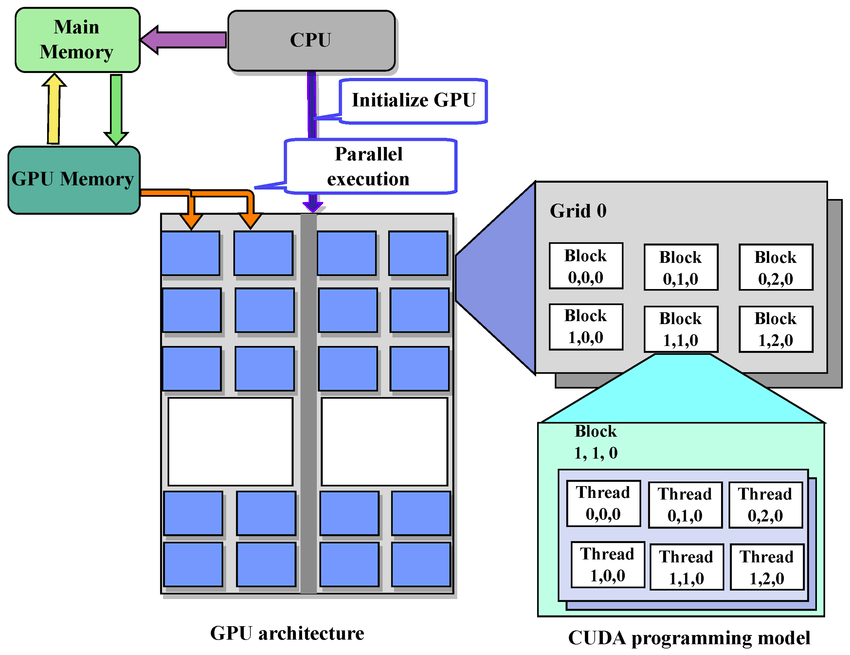
\includegraphics[width=0.8\linewidth,height=\textheight,keepaspectratio]{gpu-internal-architecture.png}
      \caption{Organização interna de GPU moderna e modelo de programação
            CUDA. Adaptado de
            \textcite{shah2023gpuarchitectureimage}.}\label{fig:gpu-internal}
\end{figure}

Essas três figuras servem como pano de fundo para as decisões de projeto dos \emph{kernels} CUDA apresentados no \capref{cap3-materiais-metodos}: explorar paralelismo em dados (Tipo~1) mapeando \emph{threads} para indivíduos ou movimentos \(2\)-opt, evitar ao máximo divergência dentro de um mesmo \emph{warp} e organizar as leituras e escritas na memória global para aproveitar melhor a largura de banda disponível.

É fundamental distinguir, portanto, três níveis de paralelismo que aparecem neste trabalho.
No nível da máquina, a CPU é tratada como uma arquitetura MIMD: diferentes núcleos podem executar tarefas distintas ou \emph{threads} independentes.
Dentro de cada núcleo, porém, a CPU pode explorar SIMD por meio de instruções vetoriais, o que acelera trechos específicos do cálculo de custos e de manipulação de vetores.
Já a GPU, no contexto de CUDA, é programada no modelo SIMT: o programador escreve milhares de \emph{threads} lógicas, mas o hardware as executa em grupos (\emph{warps}) que avançam de forma coordenada enquanto compartilham o mesmo fluxo de instruções.
Quando há divergência de controle dentro de um \emph{warp}, os caminhos precisam ser serializados temporariamente, reduzindo a eficiência.
Essa distinção explica por que a CPU pode ser descrita, sem contradição, como MIMD com extensões SIMD, enquanto a GPU é descrita mais adequadamente como SIMT.

\section{Comparação estatística de algoritmos de otimização}\label{sec-27-comparacao-estatistica}

Meta-heurísticas estocásticas, como AGs e algoritmos meméticos, produzem resultados que variam de uma execução para outra devido à aleatoriedade presente na inicialização, na seleção e na mutação.
Por isso, a avaliação comparativa não deve se apoiar em execuções isoladas nem apenas em médias aritméticas simples sem análise de variabilidade: o protocolo recomendado por \textcite{demsar2006statistical} prevê a avaliação em múltiplas instâncias independentes, com várias repetições por combinação algoritmo--instância e uso de testes não paramétricos baseados em postos.

De forma intuitiva, um teste de hipóteses ajuda a separar diferenças consistentes da variação aleatória.
Define-se inicialmente a \textbf{hipótese nula} (\(H_0\)), segundo a qual os algoritmos têm desempenho equivalente e eventuais diferenças observadas vêm apenas do acaso.
Em seguida, fixa-se um \textbf{nível de significância} \(\alpha\), que representa o limite máximo aceitável para o risco de rejeitar \(H_0\) por engano quando ela é verdadeira (erro do Tipo~I).
A partir dos dados experimentais, calcula-se o \textbf{valor-\(p\)}, que mede a probabilidade de observar uma diferença igual ou maior que a encontrada caso \(H_0\) fosse verdadeira.
Quando \(p < \alpha\), rejeita-se \(H_0\) e conclui-se que há diferença estatisticamente significativa entre os algoritmos; quando \(p \ge \alpha\), não há evidência suficiente para afirmar que eles diferem.

Para comparar algoritmos de otimização entre diferentes problemas, \textcite{demsar2006statistical} recomenda \textbf{testes não paramétricos baseados em postos (\emph{ranks})} em vez de testes paramétricos clássicos, como o teste \(t\) de Student ou a análise de variância (ANOVA).
No TSP e em otimização combinatória, tempos de execução e custos de rota variam fortemente de uma instância para outra e costumam apresentar distribuições assimétricas ou valores discrepantes (\emph{outliers}).
Testes paramétricos assumem normalidade dos dados e homogeneidade de variâncias, além de utilizarem diretamente as médias numéricas, podendo ser facilmente distorcidos por uma única instância mais difícil; além disso, condicionar a escolha do teste a pré-testes de normalidade distorce o nível de significância nominal e perde poder em amostras moderadas \autocite{demsar2006statistical}.
Já os testes baseados em postos convertem os valores numéricos em posições ordenadas (\(1^\circ, 2^\circ, \dots\)), avaliando a consistência relativa entre os métodos sem depender da forma da distribuição.

\subsection{Comparações pareadas}\label{sec-271-comparacoes-pareadas}

Na comparação entre dois algoritmos avaliados sobre os mesmos problemas --- ou sobre as mesmas sementes aleatórias em uma instância ---, \textcite[Seção~3.1.2]{demsar2006statistical} recomenda o teste não paramétrico de postos sinalizados de Wilcoxon \autocite{wilcoxon1945individual} em lugar do teste \(t\)-pareado de Student \autocite{student1908probable}.

De maneira simples, o teste de Wilcoxon funciona em três passos.
Primeiro, calcula-se a diferença de desempenho entre os dois algoritmos em cada par avaliado.
Em seguida, descartam-se os empates exatos (diferença igual a zero) e ordenam-se as diferenças restantes pelo seu valor absoluto, da menor para a maior, atribuindo-lhes postos (\(1, 2, 3, \dots\)).
Por fim, devolve-se a cada posto o sinal original da diferença (positivo quando o primeiro algoritmo foi melhor, negativo quando o segundo foi melhor) e somam-se separadamente os postos positivos e os negativos.
Se os dois algoritmos forem equivalentes (\(H_0\)), essas duas somas tendem a ficar equilibradas; se um algoritmo superar o outro de forma consistente e com as maiores margens, uma das somas dominará a outra.
Esse mecanismo aproveita a magnitude relativa das diferenças sem permitir que um único valor extremo domine o resultado.

\subsection{Comparações múltiplas}\label{sec-272-comparacoes-multiplas}

Quando três ou mais algoritmos são avaliados em várias instâncias, compará-los diretamente par a par com vários testes isolados aumentaria muito a chance de encontrar falsos positivos por puro acaso.
Para evitar esse problema, \textcite[Seção~3.2]{demsar2006statistical} recomenda o teste global (\emph{omnibus}) não paramétrico de Friedman \autocite{friedman1937use}, que avalia todos os algoritmos de uma só vez.
Dentro de cada instância, os algoritmos são classificados do melhor (\(1^\circ\) lugar) ao pior (em caso de empate, dividem a média das posições) e calcula-se o posto médio de cada algoritmo ao longo de todas as instâncias.
Se todos os métodos tiverem desempenho similar (\(H_0\)), seus postos médios ficarão próximos entre si; se algum método ficar sistematicamente nas primeiras ou últimas posições, a diferença entre os postos médios será grande.
Como a estatística original \(\chi_F^2\) de Friedman tende a ser conservadora --- dificultando a detecção de diferenças reais em conjuntos moderados de instâncias ---, \textcite{demsar2006statistical} recomenda a correção \(F_F\) de Iman--Davenport, que segue uma distribuição \(F\) mais precisa.

Como o teste de Friedman é um teste global (\emph{omnibus}), quando ele rejeita \(H_0\) (\(p < \alpha\)), ele informa apenas que \emph{existe diferença} no conjunto de algoritmos, sem apontar \emph{quais pares específicos} diferem entre si.
Para identificar esses pares controlando a probabilidade de erro global nas comparações múltiplas (isto é, o risco acumulado de obter ao menos um falso positivo no conjunto de testes), \textcite[Seção~3.2.2]{demsar2006statistical} distingue dois cenários:
\begin{enumerate}
      \item \textbf{Comparações entre todos os pares (\emph{all-pairs}):} Utiliza-se o pós-teste de Nemenyi \autocite{nemenyi1963distribution}, que calcula uma \textbf{diferença crítica} (\(CD\)) mínima entre postos médios. Dois algoritmos só são considerados estatisticamente diferentes se a distância entre seus postos médios superar \(CD\), resultado que pode ser visualizado diretamente em diagramas de diferença crítica.
      \item \textbf{Comparações contra um algoritmo de referência (controle):} Quando o objetivo é comparar os métodos avaliados com uma única linha de base de referência, o teste de Nemenyi torna-se conservador demais por descontar todos os pares possíveis. Nesse caso, \textcite{demsar2006statistical} recomenda aplicar testes pareados (como o de Wilcoxon) combinados com o ajuste sequencial (\emph{step-down}) de Holm--Bonferroni \autocite{holm1979simple}: ordenam-se os valores-\(p\) obtidos do menor para o maior e compara-se cada um com limiares progressivamente menos rigorosos (\(\alpha/c, \alpha/(c-1), \dots\)), garantindo o controle do erro global com maior poder de detecção.
\end{enumerate}

A aplicação concreta desse protocolo ao delineamento experimental deste trabalho é detalhada na \secref{sec-34-protocolo-estatistico} do \capref{cap3-materiais-metodos}, em conjunto com a estrutura das variantes descrita na \secref{sec-32-arquitetura-variantes}.

\chapter{Materiais e Métodos}\label{cap3-materiais-metodos}

Este capítulo descreve o ambiente computacional, o \emph{framework} experimental e o protocolo de execução utilizados para comparar as quatro variantes do algoritmo memético AG+\(2\)-opt apresentadas na \secref{sec-14-objetivos-especificos}.
O objetivo é permitir que outros pesquisadores reproduzam, com o máximo de precisão possível, os experimentos discutidos no \capref{cap4-resultados}, respeitando as limitações de hardware disponíveis.

\section{Ambiente computacional e \emph{framework} experimental}\label{sec-31-ambiente-framework}

Esta seção detalha as características do hardware e do software utilizados, bem como a arquitetura do \emph{framework} experimental desenvolvido para garantir a integridade e a reprodutibilidade das comparações.

\subsection{Hardware e restrições físicas}\label{sec-311-hardware-software}

Os experimentos foram conduzidos em um \emph{notebook} equipado com processador \textbf{Intel Core i7-7700HQ} e uma GPU \textbf{NVIDIA GeForce GTX 1050 Mobile}.
Trata-se de uma GPU dedicada de entrada para \emph{notebooks}, baseada na arquitetura \textbf{Pascal}.

Embora o uso deste equipamento tenha sido motivado inicialmente pela disponibilidade, o conjunto experimental oferece uma vantagem metodológica: a combinação de uma CPU \emph{quad-core} relativamente mais capaz com uma GPU de porte modesto acentua o custo de comunicação e os limites de memória, tornando as diferenças entre estratégias mais nítidas.
Por outro lado, a seleção experimental foi limitada a instâncias de até \(n_{coords} = \maiorinstancia\) cidades (\texttt{pr1002}) devido ao tempo de execução da variante de referência em CPU.
Como o protocolo estatístico exige \(n_{reps} = \totalrepeticoes\) execuções independentes de cada variante por problema, instâncias acima desse porte tornariam proibitivo o tempo de coleta da implementação puramente em CPU, cujo processamento sequencial dos indivíduos na busca local \(2\)-opt --- somado ao crescimento do número de gerações até a convergência --- eleva acentuadamente o custo computacional total.

As especificações relevantes do ambiente computacional utilizado nos experimentos estão sintetizadas na \tabref{tbl:hardware-specs}, destacando o contraste entre os \(4\) núcleos (\(8\) \emph{threads}) da CPU e os \(640\) núcleos CUDA da GPU distribuídos em \(5\) SMs (\emph{Streaming Multiprocessors}).

\begin{table}[htb]
      \centering
      \caption{Especificações do ambiente computacional utilizado nos experimentos}\label{tbl:hardware-specs}
      \begin{tabelapadrao}
            \begin{tabular}{@{}
                        >{\raggedright\arraybackslash}p{(\linewidth - 4\tabcolsep) * \real{0.2600}}
                        >{\raggedright\arraybackslash}p{(\linewidth - 4\tabcolsep) * \real{0.3400}}
                        >{\raggedright\arraybackslash}p{(\linewidth - 4\tabcolsep) * \real{0.4000}}@{}}
                  \toprule
                  Característica        & CPU (Intel Core i7-7700HQ)                                              & GPU (NVIDIA GeForce GTX 1050 Mobile)                     \\
                  \midrule
                  Arquitetura / Geração & Kaby Lake (2017)                                                        & Pascal GP107 (2016, Compute Capability 6.1)              \\
                  Núcleos / Unidades    & \(4\) núcleos / \(8\) \emph{threads}                                    & \(640\) núcleos CUDA em \(5\) SMs                        \\
                  Frequência            & \(2{,}80\)--\(3{,}80\text{ GHz}\)                                       & \(1354\)--\(1493\text{ MHz}\)                            \\
                  Memória               & \(16\text{ GB}\) RAM DDR4                                               & \(4\text{ GB}\) VRAM GDDR5 (\(\approx 112\text{ GB/s}\)) \\
                  Interface CPU--GPU    & \multicolumn{2}{c@{}}{Barramento PCIe 3.0 (\(\approx 16\text{ GB/s}\))}                                                            \\
                  \bottomrule
            \end{tabular}
      \end{tabelapadrao}
\end{table}

O desempenho computacional é estritamente limitado pelas fronteiras físicas da GPU.
Detalha-se a seguir o impacto dessas restrições no processamento:

\begin{enumerate}
      \item
            \textbf{Memória de vídeo (VRAM) e memória compartilhada:} A GPU dispõe de \(4\text{ GB}\) de VRAM.
            Seguindo a convenção da TSPLIB \autocite{reinelt1991tsplib}, tanto a matriz completa de distâncias \(D\) (\(n_{coords}^2\) elementos) quanto os dois \emph{buffers} de população (\(2 \times n_{pop} \times n_{coords}\) elementos, com \(n_{pop} = 256\)) são armazenados como inteiros de \(32\) bits (\texttt{int32}, \(4\) bytes cada), enquanto o vetor de custos usa inteiros de \(64\) bits (\(256 \times 8 = 2048\) bytes).
            Na variante Totalmente em GPU, que mantém todo o estado residente na placa, o consumo de VRAM é dado por:
            \begin{equation}\label{eq:vram-total}
                  Mem_{total}(n_{coords}) \approx 4\,n_{coords}^2 + 2048\,n_{coords} + 2048 \text{ bytes.}
            \end{equation}
            Mesmo na maior instância testada (\(n_{coords} = \maiorinstancia\), \texttt{pr1002}), a Equação~\eqref{eq:vram-total} resulta em cerca de \(6{,}07\text{ MB}\) --- uma fração mínima dos \(4\text{ GB}\) disponíveis.
            Além disso, a janela de memória compartilhada dos blocos comporta rotas de até \(2048\) cidades, de modo que todas as \totalinstancias\ instâncias deste estudo cabem inteiramente na memória rápida local sem necessidade de particionamento.
      \item
            \textbf{Comunicação CPU--GPU via barramento PCIe:} A troca de dados entre CPU e GPU ocorre pelo barramento PCIe, cuja largura de banda (\(\approx 16\text{ GB/s}\)) é cerca de sete vezes menor que a largura de banda interna da VRAM (\(\approx 112\text{ GB/s}\)).
            Transferências frequentes penalizam diretamente o tempo total de execução conforme a decomposição:
            \begin{equation}\label{eq:tempo-total}
                  T_{total} = T_{cpu} + T_{gpu} + T_{transf}\text{,}
            \end{equation}
            podendo anular o ganho obtido nos núcleos gráficos.
            Esse contraste motiva reduzir o número de transferências por geração (\textbf{Híbrida Otimizada}) ou manter todo o ciclo evolutivo na GPU (\textbf{Totalmente em GPU}), conforme detalhado na \secref{sec-322-variantes}.
      \item
            \textbf{Ocupação dos \(640\) núcleos CUDA (\(5\) SMs):} Manter centenas de \emph{threads} ativas simultaneamente nos \(5\) \emph{SMs}\footnote{\textbf{Limite arquitetural da GPU utilizada:} Na microarquitetura Pascal (Compute Capability 6.1) da GTX~1050 Mobile, cada SM suporta no máximo \(2048\) \emph{threads} residentes (\(64\) \emph{warps}); em outras gerações de GPU esse teto difere.
            O uso elevado de registradores ou de memória compartilhada por bloco reduz a ocupação efetiva abaixo desse limite.}
            (\emph{Streaming Multiprocessors}) --- cada um com 128 cores, totalizando 640 núcleos de execução --- permite que os multiprocessadores alternem a execução entre grupos de \emph{threads} prontos enquanto outros aguardam leituras de memória, ocultando a latência de acesso (\emph{latency hiding}) e sustentando alta taxa de ocupação dos \(640\) núcleos \autocite{kirk2010programming}.
\end{enumerate}

\subsection{Ambiente de software}\label{sec-312-ambiente-software}

O \emph{framework} experimental foi desenvolvido em \texttt{Python 3.12.13} sobre \texttt{Debian GNU/Linux 13}, utilizando um conjunto de bibliotecas e compiladores selecionados para assegurar consistência funcional entre as execuções em CPU e GPU.
As versões exatas, os requisitos mínimos de arquitetura CUDA e o papel de cada componente central constam na \tabref{tbl:software-specs}.

\begin{table}[htb]
      \centering
      \caption{Especificações, requisitos mínimos e papel dos componentes do ambiente de software}\label{tbl:software-specs}
      \begin{tabelapadrao}
            \begin{tabular}{@{}
                        >{\raggedright\arraybackslash}p{(\linewidth - 4\tabcolsep) * \real{0.2600}}
                        >{\raggedright\arraybackslash}p{(\linewidth - 4\tabcolsep) * \real{0.3400}}
                        >{\raggedright\arraybackslash}p{(\linewidth - 4\tabcolsep) * \real{0.4000}}@{}}
                  \toprule
                  Componente                     & Versão / Requisito                                             & Papel no ambiente                                                     \\
                  \midrule
                  Sistema operacional            & Debian GNU/Linux 13 (\emph{trixie}), kernel 6.12.43 (\texttt{x86\_64}) & Plataforma de execução do \emph{benchmark}                            \\
                  \sepitem
                  \emph{Driver} gráfico NVIDIA   & 580.196.07                                                     & Interface com a GPU e suporte ao CUDA Runtime 12.9                    \\
                  \sepitem
                  CUDA Toolkit / compilador      & CUDA 12.9 (\texttt{nvcc} V12.9.86)                             & Compilação e execução dos \emph{kernels} CUDA customizados            \\
                  \sepitem
                  Compute Capability CUDA        & Mínimo \(\ge 5{,}0\) (testado: \(6{,}1\), Pascal)              & Requisito mínimo do CUDA 12.9 e do \texttt{cupy-cuda12x}              \\
                  \sepitem
                  Compilador C/C++ (\emph{host}) & GCC 12.4.0                                                     & Compilador auxiliar de \emph{host} exigido pelo \texttt{nvcc}         \\
                  \sepitem
                  Interpretador Python           & Python 3.12.13 (mínimo \(\ge 3{,}12\))                         & Orquestração dos experimentos e interface com CPU/GPU                 \\
                  \sepitem
                  Computação numérica            & NumPy 2.5.4; \hyperlink{term:cupy}{CuPy} 14.2.0                & \emph{Backend} de CPU (NumPy) e GPU (CuPy sobre CUDA 12.9)            \\
                  \sepitem
                  Estatística e banco de dados   & SciPy 1.18.1; scikit-posthocs 0.17.1; DuckDB 2.0.0             & Protocolo de \textcite{demsar2006statistical} e consolidação (\apref{apendice-banco}) \\
                  \bottomrule
            \end{tabular}
      \end{tabelapadrao}
\end{table}

A compatibilidade de API entre NumPy e CuPy foi determinante para manter a lógica algorítmica idêntica entre as variantes de CPU e GPU, alterando apenas o \emph{backend} de execução.
Os demais pacotes auxiliares de análise, visualização e validação declarados no projeto, bem como o procedimento reproduzível de instalação do ambiente via \texttt{uv}, estão documentados no \apref{apendice-reproducao}.

Embora a API de alto nível do CuPy seja adequada para operações matriciais regulares, na variante \textbf{Totalmente em GPU} (\texttt{FullGPUModular}) tanto a busca local \(2\)-opt quanto os operadores genéticos (seleção por torneio, cruzamento OX, mutação por troca e avaliação de custo) são executados por \textbf{kernels CUDA customizados} escritos em C++ (\texttt{RawKernel}).
O desenvolvimento direto desses \emph{kernels} evita sobrecargas repetidas de chamadas da API de alto nível e viabiliza três ganhos estruturais:

\begin{enumerate}
      \item
            \textbf{Fusão e encadeamento de etapas na GPU:} Executar o refinamento \(2\)-opt, a avaliação de custos e os operadores evolutivos diretamente na GPU, evitando retornos intermediários à CPU.
      \item
            \textbf{Uso explícito da memória rápida local:} Armazenar dados ativos das rotas e estruturas auxiliares na memória compartilhada dos blocos e em registradores, reduzindo acessos à memória global.
      \item
            \textbf{Cooperação entre \emph{threads} na busca \(2\)-opt:} Em vez de limitar cada rota a uma única \emph{thread} isolada, os \emph{kernels} customizados permitem que múltiplas \emph{threads} de um mesmo bloco cooperem na avaliação dos movimentos candidatos de cada rota e processem toda a matriz de rotas da população de uma só vez.
\end{enumerate}

A avaliação de custos usa \textbf{aritmética inteira}.
O arredondamento da TSPLIB é aplicado uma única vez, ao montar a matriz de distâncias \(D\), por \(\text{nint}(x) = \lfloor x + 0{,}5 \rfloor\), conforme o tipo de cada instância (por exemplo, a distância euclidiana em \texttt{EUC\_2D}, com regras próprias em \texttt{CEIL\_2D}, \texttt{ATT} e \texttt{GEO}) \autocite{reinelt1991tsplib}.
A partir desse ponto, todas as distâncias entre cidades são números inteiros de \(32\) bits (\texttt{int32}) e o custo total de qualquer circuito é acumulado em \(64\) bits (\texttt{int64}), o que evita ultrapassar o limite de representação de \(32\) bits em rotas de grande porte.
Consequentemente, o custo de qualquer rota candidata e o ganho \(\Delta C\) de qualquer troca \(2\)-opt reduzem-se a somas e subtrações exatas de inteiros, eliminando divergências de arredondamento de ponto flutuante entre CPU e GPU e garantindo que duas variantes quaisquer atribuam \textbf{exatamente o mesmo custo} a uma mesma rota.

\subsection{Arquitetura do \emph{framework} experimental}\label{sec-313-arquitetura-framework}

Para garantir comparações justas, o código foi estruturado em uma arquitetura modular que separa a lógica dos algoritmos da orquestração dos experimentos.
O \emph{framework} opera em três camadas distintas, ilustradas na \figref{fig:class-diagram}:

\begin{enumerate}
      \item
            \textbf{Camada de Algoritmos:} Adota um padrão modular de estratégias intercambiáveis em torno de uma única classe orquestradora (\texttt{GeneticAlgorithm}), cujas seis etapas do ciclo evolutivo recebem implementações de CPU ou de GPU sob o mesmo contrato; a definição detalhada das quatro variantes é apresentada na \secref{sec-32-arquitetura-variantes}.
      \item
            \textbf{Camada de Orquestração (\hyperlink{term:benchmark}{Benchmark}):} Responsável por carregar as configurações experimentais (parâmetros, instâncias), gerenciar a execução das repetições independentes e garantir o isolamento entre testes.
            Esta camada implementa mecanismos de \emph{checkpoint} para salvar o estado de cada execução, permitindo a recuperação em caso de falhas e a auditoria posterior dos dados.
      \item
            \textbf{Camada de Análise Estatística e Visualização:} Scripts dedicados a processar os \emph{checkpoints}, consolidar os dados e gerar as tabelas, diagramas e relatórios estatísticos.
\end{enumerate}

\begin{figure}[htbp]
      \centering
      \caption{Arquitetura modular em três camadas do \emph{framework} experimental}\label{fig:class-diagram}
      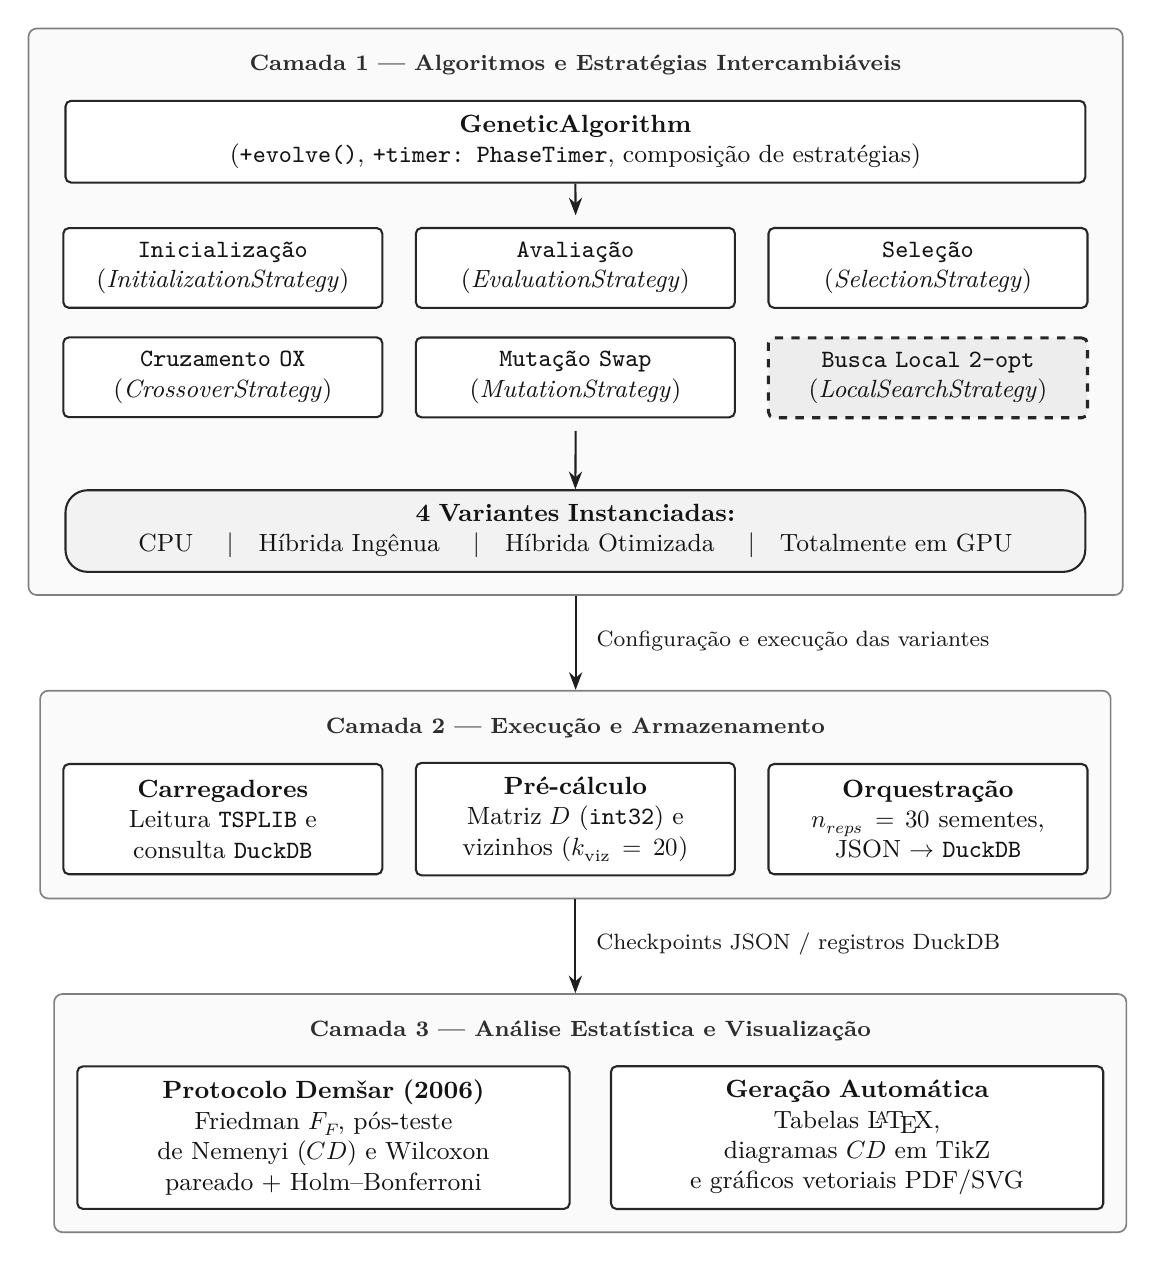
\begin{tikzpicture}[node distance=5mm and 4mm]
            % CAMADA 1: Algoritmos e Estrategias
            \node[fc_proc, text width=12.6cm] (solver) {\textbf{GeneticAlgorithm}\\(\texttt{+evolve()}, \texttt{+timer: PhaseTimer}, composição de estratégias)};
            \node[fc_grouptitle, above=2.5mm of solver] (tc1) {Camada 1 — Algoritmos e Estratégias Intercambiáveis};
            \node[fc_proc, below=5.5mm of solver, text width=3.7cm] (s2) {\texttt{Avaliação}\\(\emph{EvaluationStrategy})};
            \node[fc_proc, left=4mm of s2, text width=3.7cm] (s1) {\texttt{Inicialização}\\(\emph{InitializationStrategy})};
            \node[fc_proc, right=4mm of s2, text width=3.7cm] (s3) {\texttt{Seleção}\\(\emph{SelectionStrategy})};
            \node[fc_proc, below=3.5mm of s1, text width=3.7cm] (s4) {\texttt{Cruzamento OX}\\(\emph{CrossoverStrategy})};
            \node[fc_proc, below=3.5mm of s2, text width=3.7cm] (s5) {\texttt{Mutação Swap}\\(\emph{MutationStrategy})};
            \node[fc_memetic, below=3.5mm of s3, text width=3.7cm] (s6) {\texttt{Busca Local 2-opt}\\(\emph{LocalSearchStrategy})};
            \node[fc_term, below=9mm of s5, text width=12.6cm] (vars) {\textbf{4 Variantes Instanciadas:}\\CPU \quad\textbar\quad Híbrida Ingênua \quad\textbar\quad Híbrida Otimizada \quad\textbar\quad Totalmente em GPU};

            % CAMADA 2: Execução e Armazenamento (titulo centralizado dentro do topo, seta central sem colisão)
            \node[fc_proc, below=24mm of vars, text width=3.7cm, minimum height=14mm] (l2b) {\textbf{Pré-cálculo}\\Matriz \(D\) (\texttt{int32}) e\\vizinhos (\(k_{\text{viz}} = \kviz\))};
            \node[fc_proc, left=4mm of l2b, text width=3.7cm, minimum height=14mm] (l2a) {\textbf{Carregadores}\\Leitura \texttt{TSPLIB} e\\consulta \texttt{DuckDB}};
            \node[fc_proc, right=4mm of l2b, text width=3.7cm, minimum height=14mm] (l2c) {\textbf{Orquestração}\\\(n_{reps} = \totalrepeticoes\) sementes,\\JSON \(\to\) \texttt{DuckDB}};
            \node[fc_grouptitle, above=2.5mm of l2b] (tc2) {Camada 2 — Execução e Armazenamento};

            % CAMADA 3: Analise Estatística e Visualização (simétrico em x=0: (5.9+0.5)/2 = 3.2cm)
            \node[fc_proc, below=24mm of l2b, xshift=-3.2cm, text width=5.9cm, minimum height=14mm] (l3a) {\textbf{Protocolo Demšar (2006)}\\Friedman \(F_F\), pós-teste\\de Nemenyi (\(CD\)) e Wilcoxon\\pareado + Holm--Bonferroni};
            \node[fc_proc, right=5mm of l3a, text width=5.9cm, minimum height=14mm] (l3b) {\textbf{Geração Automática}\\Tabelas \LaTeX,\\diagramas \(CD\) em TikZ\\e gráficos vetoriais PDF/SVG};
            \node[fc_grouptitle, above=2.5mm of $(l3a.north)!0.5!(l3b.north)$] (tc3) {Camada 3 — Análise Estatística e Visualização};

            % Caixas de camada
            \begin{scope}[on background layer]
                  \node[draw=black!35, dashed, rounded corners=2pt, fill=white, inner sep=4pt, fit=(s1)(s2)(s3)(s4)(s5)(s6)] (sgrid) {};
                  \node[fc_group, fit=(tc1)(solver)(sgrid)(vars)] (c1) {};
                  \node[fc_group, fit=(tc2)(l2a)(l2b)(l2c)] (c2) {};
                  \node[fc_group, fit=(tc3)(l3a)(l3b)] (c3) {};
            \end{scope}

            % Redesenha títulos por cima do fundo
            \node[fc_grouptitle] at (tc1) {Camada 1 — Algoritmos e Estratégias Intercambiáveis};
            \node[fc_grouptitle] at (tc2) {Camada 2 — Execução e Armazenamento};
            \node[fc_grouptitle] at (tc3) {Camada 3 — Análise Estatística e Visualização};

            % Conexões centralizadas e estritamente verticais
            \draw[fc_arr] (solver.south) -- (sgrid.north);
            \draw[fc_arr] (sgrid.south) -- (vars.north);
            \draw[fc_arr] (c1.south) -- node[fc_lbl, right=2mm, pos=0.48] {Configuração e execução das variantes} (c1.south |- c2.north);
            \draw[fc_arr] (c2.south) -- node[fc_lbl, right=2mm, pos=0.48] {Checkpoints JSON / registros DuckDB} (c2.south |- c3.north);
      \end{tikzpicture}
\end{figure}

Esta separação assegura que as métricas de tempo e qualidade sejam coletadas de forma consistente para todas as variantes, eliminando vieses que poderiam surgir de implementações \emph{ad hoc} para cada plataforma.

\section{Variantes algorítmicas e estratégias de paralelização}\label{sec-32-arquitetura-variantes}

As variantes comparadas neste trabalho são \textbf{análogas}.
Todas partem do mesmo algoritmo memético, com os mesmos operadores, os mesmos hiperparâmetros globais e os mesmos critérios de parada, e diferem em \emph{onde} cada etapa é executada --- CPU ou GPU --- e em \emph{como} os dados trafegam e são processados: sequencialmente na CPU, por circuito individual \(C_m\) ou pela matriz completa da população \(P(t)\) (\secref{sec-322-variantes}).
Paralelizar muda o modo de execução, e é por isso que as variantes são tratadas como análogas, e não como equivalentes.
A assimetria de avaliação entre CPU e GPU --- bem como a equivalência bit a bit verificada entre as variantes híbridas --- é detalhada na \secref{sec-5311-semantica-operadores}.

\subsection{O algoritmo genético base (AG + \texorpdfstring{\(2\)-opt}{2-opt})}\label{sec-321-ga-base}

O algoritmo base é um Algoritmo Genético (AG) com seleção elitista de sobreviventes do tipo \((\mu + \lambda)\), na qual pais e descendentes têm o mesmo tamanho (\(\mu = \lambda = n_{pop}\)), hibridizado com uma busca local \(2\)-opt truncada.
Esta combinação, denominada Algoritmo Memético, equilibra a exploração global do espaço de busca (via operadores genéticos) com a intensificação local (via \(2\)-opt).
Todos os hiperparâmetros mantidos constantes nas quatro variantes constam na \tabref{tbl:ga-hyperparameters} e são detalhados a seguir:

\begin{table}[htbp]
      \centering
      \caption{Hiperparâmetros e configurações fixas do algoritmo memético AG+\(2\)-opt adotados nas quatro variantes}\label{tbl:ga-hyperparameters}
      \begin{tabelapadrao}
            \begin{tabular}{@{}
                        >{\raggedright\arraybackslash}p{(\linewidth - 4\tabcolsep) * \real{0.3400}}
                        >{\centering\arraybackslash}p{(\linewidth - 4\tabcolsep) * \real{0.1600}}
                        >{\raggedright\arraybackslash}p{(\linewidth - 4\tabcolsep) * \real{0.5000}}@{}}
                  \toprule
                  Parâmetro / Componente                  & Símbolo                    & Valor / Especificação                                                                      \\
                  \midrule
                  Tamanho da população                    & \(n_{pop}\)                & \(256\) rotas                                                                              \\
                  Seleção de progenitores                 & \(\tau_{\text{trnmt}}\)    & Torneio de tamanho \(5\)                                                                   \\
                  Cruzamento (\emph{Order Crossover}, OX) & \(p_c\)                    & \(1{,}0\) (aplicado a todos os \(n_{pop}/2\) pares)                                        \\
                  Mutação por troca (\emph{swap})         & \(p_{\text{mut}}\)         & \(0{,}02\) por rota descendente                                                            \\
                  Busca local \(2\)-opt (pós-mutação)     & \(\kappa\)                 & Até \(\maxpassadas\) varreduras \emph{best-improvement}                                    \\
                  Lista estática de candidatos            & \(k_{\text{viz}}\)         & \(\kviz\) vizinhos mais próximos por cidade                                                \\
                  Seleção de sobreviventes (elitismo)     & \((\mu + \lambda)\)        & Determinística com \(\mu = \lambda = 256\) (melhores \(256\) de \(512\))                   \\
                  Critério de parada (i) --- alvo         & \(\varepsilon_{\text{alvo}}\) & \(\text{gap} \le 1\%\) em relação a \(B^*\)                                             \\
                  Critério de parada (ii) --- estagnação  & \(G_{\text{estag}}\)       & \(\lceil 2\sqrt{n_{coords}} \rceil\) gerações sem melhoria                                 \\
                  Critério de parada (iii) --- teto       & \(G_{\max}\)               & \(\lceil 2\,n_{coords}\sqrt{n_{coords}} \rceil\) gerações                                  \\
                  Repetições e sementes                   & \(n_{reps}\)               & \(\totalrepeticoes\) execuções (sementes inteiras \(\sementeinicial\) a \(\sementefinal\)) \\
                  \bottomrule
            \end{tabular}
      \end{tabelapadrao}
\end{table}

As escolhas de projeto subjacentes aos parâmetros da \tabref{tbl:ga-hyperparameters} obedecem a três diretrizes técnicas:

\begin{itemize}
      \item
            \textbf{Escala de memória da população (\(n_{pop} = 256\)):} O tamanho fixo enquadra-se na faixa usual de \(50\) a \(500\) indivíduos da literatura de AGs para o TSP \autocite{harik1999gambler,goldberg1992massive,larranaga1999genetic} e equilibra a ocupação em VRAM. Enquanto a matriz de distâncias cresce quadraticamente (\(\mathcal{O}(n_{coords}^2)\), ocupando \(4\,n_{coords}^2\) bytes), a população cresce bilinearmente (\(\mathcal{O}(n_{pop}\,n_{coords})\), ocupando \(4\,n_{pop}\,n_{coords}\) bytes por \emph{buffer}), mantendo o custo de uma população abaixo de \(1\text{ MiB}\) (\(\approx 1{,}03\text{ MB}\)) até \(n_{coords} = \maiorinstancia\) e evitando que um \(n_{pop}\) proporcional a \(n_{coords}\) introduza um segundo termo quadrático na memória do dispositivo.
      \item
            \textbf{Representação e operadores evolutivos:} As rotas são codificadas como permutações de inteiros sem repetição; a seleção por torneio independe de reescalonamento global de aptidão e paraleliza-se diretamente por sorteios independentes; o operador OX preserva a ordem relativa de sub-rotas válidas ao recombinar cada par de progenitores; e a mutação por troca (\emph{swap}) introduz perturbações mínimas mantendo a factibilidade do circuito.
      \item
            \textbf{Acoplamento pós-mutação e lista estática de vizinhos (\(k_{\text{viz}} = \kviz\)):} A busca local \(2\)-opt \emph{best-improvement} é aplicada sobre cada descendente pós-mutação \autocite{alsheddy2017memetic,larranaga1999genetic} com vizinhança restrita aos \(k_{\text{viz}} = \kviz\) vizinhos mais próximos (\secref{sec-221-2opt}), encerrando-se o ciclo evolutivo assim que qualquer um dos três critérios de parada listados na \tabref{tbl:ga-hyperparameters} é satisfeito.
\end{itemize}

Para justificar empiricamente a escolha de \(k_{\text{viz}} = \kviz\), realizou-se um microbenchmark isolado com \(64\) rotas e \(\kappa = \maxpassadas\) varreduras de \(2\)-opt comparando a lista de candidatos contra a varredura exaustiva completa, cujos resultados constam na \tabref{tbl:candidate-k-microbenchmark}.
Em instâncias muito pequenas (\texttt{berlin52}), o custo de indireção da tabela empata com a varredura direta (\(0{,}99\times\) na CPU; \(0{,}79\times\) na GPU), mas já a partir de \(n_{coords} = 100\) a restrição de vizinhança acelera a busca local em até \(8{,}22\times\) na CPU (\texttt{pr264}) e \(4{,}05\times\) na GPU (\texttt{lin318}), viabilizando a execução completa da linha de base em CPU até \(n_{coords} = \maiorinstancia\) sob exatamente o mesmo orçamento de busca.

\begin{table}[htbp]
      \centering
      \caption{Microbenchmark isolado da restrição por lista de candidatos (\(k_{\text{viz}} = \kviz\) vs.\ varredura exaustiva, \(64\) rotas, \(\kappa = \maxpassadas\) passadas)}\label{tbl:candidate-k-microbenchmark}
      \begin{tabelapadrao}
            \begin{tabular}{@{}lrrrrrr@{}}
                  \toprule
                  Instância                    & \multicolumn{3}{c}{CPU (s)} & \multicolumn{3}{c}{GPU -- matriz de rotas (s)}                                                                                  \\
                  \cmidrule(lr){2-4} \cmidrule(lr){5-7}
                                               & \(k_{\text{viz}} = \kviz\)  & Exaustiva                                      & Ganho            & \(k_{\text{viz}} = \kviz\) & Exaustiva   & Ganho            \\
                  \midrule
                  \texttt{berlin52} (\(n=52\)) & \(0{,}935\)                 & \(0{,}924\)                                    & \(0{,}99\times\) & \(0{,}001\)                & \(0{,}001\) & \(0{,}79\times\) \\
                  \texttt{kroA100} (\(n=100\)) & \(1{,}590\)                 & \(4{,}250\)                                    & \(2{,}67\times\) & \(0{,}002\)                & \(0{,}003\) & \(1{,}51\times\) \\
                  \texttt{ch150} (\(n=150\))   & \(3{,}122\)                 & \(8{,}066\)                                    & \(2{,}58\times\) & \(0{,}003\)                & \(0{,}005\) & \(2{,}03\times\) \\
                  \texttt{pr264} (\(n=264\))   & \(4{,}808\)                 & \(39{,}513\)                                   & \(8{,}22\times\) & \(0{,}004\)                & \(0{,}016\) & \(3{,}72\times\) \\
                  \texttt{lin318} (\(n=318\))  & \(5{,}811\)                 & \(45{,}798\)                                   & \(7{,}88\times\) & \(0{,}006\)                & \(0{,}023\) & \(4{,}05\times\) \\
                  \bottomrule
            \end{tabular}
      \end{tabelapadrao}
\end{table}

\subsection{Estratégias de paralelização (as quatro variantes)}\label{sec-322-variantes}

Para investigar o impacto da GPU, o algoritmo base foi instanciado em quatro variantes, que não são implementações separadas: todas usam o mesmo algoritmo, e a variante define apenas quais implementações ocupam cada uma das seis estratégias intercambiáveis do ciclo evolutivo --- inicialização, seleção, cruzamento, mutação, busca local e avaliação.
Conectando o ciclo conceitual de sete etapas (\secref{sec-251-ga-2opt}) à decomposição temporal em oito fases cronometradas no \capref{cap4-resultados} (\secref{sec-44-decomposicao-fases} e \apref{apendice-telemetria}), a sétima etapa --- seleção de sobreviventes elitista \((\mu + \lambda)\) --- executa na CPU nas três primeiras variantes e na GPU na variante Totalmente em GPU, enquanto a oitava fase registra explicitamente a sincronização entre CPU e GPU (\texttt{Sinc.}).

\begin{enumerate}
      \item
            \textbf{CPU (\hyperlink{term:baseline}{\emph{baseline}}):} Execução inteiramente na CPU utilizando NumPy: inicialização, seleção, cruzamento, mutação, busca local e avaliação apontam para as implementações NumPy da mesma classe \texttt{GeneticAlgorithm}.
            No nível arquitetural, a CPU permanece sendo a plataforma MIMD de referência; o que ocorre aqui é o aproveitamento pontual de vetorização SIMD dentro dos núcleos para acelerar partes da avaliação dos movimentos \(2\)-opt.
            Já o processamento dos indivíduos, no nível do algoritmo, ocorre essencialmente de forma sequencial.
            Esta variante serve como referência para medir o ganho de performance absoluto.
      \item
            \textbf{HybridNaive (Híbrida Ingênua):} Mantém a população, os operadores genéticos e a avaliação de custos na CPU, enviando apenas a busca local \(2\)-opt para a GPU.
            A cada geração, reenvia a matriz de distâncias \(D\) e transfere cada uma das \(n_{pop} = 256\) rotas individualmente (uma a uma) para a placa, disparando um lançamento de \emph{kernel} por rota e trazendo-a de volta em seguida.
            É esse envio individual --- que multiplica as transferências (\(\mathit{H2D}\) e \(\mathit{D2H}\)) e os lançamentos de \emph{kernel} em cada geração --- que caracteriza a abordagem como ``ingênua'', expondo a latência de disparo e o gargalo do barramento PCIe.
      \item
            \textbf{HybridOptimized (Híbrida Otimizada):} Também mantém os operadores genéticos na CPU, mas fixa a matriz \(D\) em VRAM e agrupa todas as rotas da população \(P(t)\) em uma única matriz (\(n_{pop} \times n_{coords}\)).
            Em cada geração, toda a população é enviada em bloco à GPU e refinada por um único lançamento do \emph{kernel} \(2\)-opt, que devolve a matriz refinada à CPU; em seguida, a avaliação de custos também roda em bloco na GPU, retornando apenas o vetor com os \(256\) custos.
            Comparada à Híbrida Ingênua, essa organização em lote elimina o reenvio repetido de \(D\) e reduz drasticamente o número de lançamentos de \emph{kernel}.
      \item
            \textbf{FullGPUModular (Totalmente em GPU):} Implementa a estratégia de ``GPU residente'': a matriz de distâncias \(D\), a lista de candidatos \(N_k\) e a população inicial \(P(0)\) (gerada sob a mesma semente compartilhada) são enviadas uma única vez na inicialização à VRAM, onde permanecem residentes enquanto todas as etapas iterativas do ciclo evolutivo --- seleção, cruzamento, mutação, busca local \(2\)-opt, avaliação e seleção de sobreviventes \((\mu + \lambda)\) --- executam na GPU.
            Essa organização elimina completamente o retorno de matrizes de rotas para a CPU (\(0{,}00\)\,MB em \(\mathit{D2H}\), restrito a escalares de parada) e reduz o tráfego recorrente \(\mathit{H2D}\) a apenas cerca de \(11{,}26\)\,KB por geração (independentemente de \(n_{coords}\)), correspondentes aos sorteios aleatórios gerados na CPU pelo NumPy (participantes dos torneios, pontos de corte do OX e posições de mutação) para manter exatamente a mesma sequência de sementes nas quatro variantes.
            Os operadores de GPU não usam as abstrações de alto nível do CuPy, e sim \emph{kernels} CUDA escritos especificamente para este trabalho e pré-compilados antes das medições.
\end{enumerate}

\section{Seleção de instâncias e protocolo experimental}\label{sec-33-selecao-instancias}

Para garantir a relevância estatística dos resultados, foram selecionadas \totalinstancias\ instâncias da biblioteca \textbf{TSPLIB} \autocite{reinelt1991tsplib}, variando de \(\menorinstancia\) a \(\maiorinstancia\) cidades, de modo a abranger diferentes escalas de dimensão no conjunto avaliado.
O conjunto inclui problemas com diferentes características geométricas e diferentes formatos de cálculo de distância (\texttt{EUC\_2D}, \texttt{ATT}, \texttt{GEO} e \texttt{EXPLICIT}) \autocite{reinelt1991tsplib}, permitindo avaliar os algoritmos em diferentes cenários.
As \totalinstancias\ instâncias selecionadas estão listadas em ordem crescente de dimensão na \tabref{tbl:selected-instances}, juntamente com seus respectivos formatos de distância e ótimos conhecidos (\(B^*\)).

\begin{tabelapadrao}
\begin{longtable}[]{@{}
            >{\raggedright\arraybackslash}p{(\linewidth - 6\tabcolsep) * \real{0.2400}}
            >{\centering\arraybackslash}p{(\linewidth - 6\tabcolsep) * \real{0.1800}}
            >{\centering\arraybackslash}p{(\linewidth - 6\tabcolsep) * \real{0.2800}}
            >{\raggedleft\arraybackslash}p{(\linewidth - 6\tabcolsep) * \real{0.3000}}@{}}
      \caption{Instâncias da TSPLIB selecionadas para o estudo}\label{tbl:selected-instances}\tabularnewline
      \toprule\noalign{}
      Instância         & \(n_{coords}\) & Tipo de distância & Ótimo conhecido (\(B^*\)) \\
      \midrule\noalign{}
      \endfirsthead
      \toprule\noalign{}
      Instância         & \(n_{coords}\) & Tipo de distância & Ótimo conhecido (\(B^*\)) \\
      \midrule\noalign{}
      \endhead
      \bottomrule\noalign{}
      \endlastfoot
      \texttt{att48}    & \(48\)         & \texttt{ATT}      & \(10628\)                 \\*
      \texttt{eil51}    & \(51\)         & \texttt{EUC\_2D}  & \(426\)                   \\*
      \texttt{berlin52} & \(52\)         & \texttt{EUC\_2D}  & \(7542\)                  \\*
      \texttt{gr96}     & \(96\)         & \texttt{GEO}      & \(55209\)                 \\*
      \texttt{kroA100}  & \(100\)        & \texttt{EUC\_2D}  & \(21282\)                 \\*
      \texttt{ch150}    & \(150\)        & \texttt{EUC\_2D}  & \(6528\)                  \\*
      \texttt{d198}     & \(198\)        & \texttt{EUC\_2D}  & \(15780\)                 \\*
      \texttt{pr264}    & \(264\)        & \texttt{EUC\_2D}  & \(49135\)                 \\*
      \texttt{lin318}   & \(318\)        & \texttt{EUC\_2D}  & \(42029\)                 \\*
      \texttt{pcb442}   & \(442\)        & \texttt{EUC\_2D}  & \(50778\)                 \\*
      \texttt{att532}   & \(532\)        & \texttt{ATT}      & \(27686\)                 \\*
      \texttt{si535}    & \(535\)        & \texttt{EXPLICIT} & \(48450\)                 \\*
      \texttt{gr666}    & \(666\)        & \texttt{GEO}      & \(294358\)                \\*
      \texttt{rat783}   & \(783\)        & \texttt{EUC\_2D}  & \(8806\)                  \\*
      \texttt{pr1002}   & \(1002\)       & \texttt{EUC\_2D}  & \(259045\)                \\
\end{longtable}
\end{tabelapadrao}

O protocolo de execução seguiu as diretrizes para comparação de algoritmos estocásticos:

\begin{itemize}
      \item
            \textbf{Repetições:} Cada par (algoritmo, instância) foi executado em \textbf{\totalrepeticoes\ repetições} independentes.
      \item
            \textbf{Sementes Aleatórias:} As sementes foram fixadas e distintas por repetição --- derivadas da semente base \(\sementeinicial\) somada ao índice da repetição (de \(\sementeinicial\) a \(\sementefinal\)) ---, o que torna cada execução reprodutível e amostra adequadamente o comportamento estocástico.
\end{itemize}

\section{Protocolo de análise estatística}\label{sec-34-protocolo-estatistico}

Aplicando os testes não paramétricos formulados na \secref{sec-27-comparacao-estatistica} \autocite{demsar2006statistical} ao nível de significância \(\alpha = 0{,}05\), avaliam-se as duas métricas centrais do estudo: a qualidade das soluções (\emph{gap} percentual frente a \(B^*\)) e o desempenho computacional (tempo de execução e \hyperlink{term:speedup}{\emph{speedup}}).
O protocolo combina dois eixos complementares sobre as \(m_{\text{alg}} = \totalvariantes\) variantes, as \(n_{\text{inst}} = \totalinstancias\) instâncias e as \(n_{reps} = \totalrepeticoes\) repetições independentes, sintetizados na \figref{fig:results-flowchart}.

\subsection{Eixo 1: comparações pareadas por instância}\label{sec-341-eixo1}

Dentro de cada uma das \(n_{\text{inst}} = \totalinstancias\) instâncias, confrontam-se todos os \(m = 6\) pares possíveis entre as \totalvariantes\ variantes sobre as \(n_{reps} = \totalrepeticoes\) execuções pareadas pelas mesmas sementes aleatórias, utilizando o teste de Wilcoxon da Equação~\eqref{eq:wilcoxon} \autocite{wilcoxon1945individual}.
Para controlar o erro do Tipo~I global nas \(m = 6\) comparações simultâneas de cada instância, os valores-\(p\) recebem o ajuste sequencial de Holm--Bonferroni (\secref{sec-272-comparacoes-multiplas}), comparando-se os valores-\(p\) ordenados aos limiares \(\alpha / (6 - i + 1)\) para \(i = 1, \dots, 6\) \autocite{holm1979simple}.
Quando mais da metade das diferenças pareadas em um par é exatamente nula (empates idênticos), registra-se o número efetivo de diferenças não nulas como alerta de poder estatístico reduzido \autocite[Seção~3.1.3]{demsar2006statistical}.

\subsection{Eixo 2: comparação global multi-instância}\label{sec-342-eixo2}

Na análise agregada, cada combinação algoritmo--instância é resumida pela média das \(n_{reps} = \totalrepeticoes\) repetições, gerando uma matriz \(N \times k\) com \(N = n_{\text{inst}} = \totalinstancias\) e \(k = m_{\text{alg}} = \totalvariantes\) para o \emph{gap} e outra para o tempo de execução.
Sobre cada matriz, calculam-se os postos médios \(R_j\) pela Equação~\eqref{eq:friedman-ranks}, a estatística de Friedman \(\chi_F^2\) pela Equação~\eqref{eq:friedman-chi2} e a estatística \(F_F\) de Iman--Davenport pela Equação~\eqref{eq:iman-davenport} (com \(3\) e \(42\) graus de liberdade) \autocite{friedman1937use,demsar2006statistical}.

Sempre que a hipótese nula global \(H_0\) é rejeitada (\(p_F < 0{,}05\)), aplica-se o pós-teste de Nemenyi pela Equação~\eqref{eq:nemenyi-cd} para comparar todos os \(6\) pares de variantes \autocite{nemenyi1963distribution}.
Substituindo \(k = \totalvariantes\), \(N = \totalinstancias\) e o valor crítico tabelado \(q_{0{,}05} = 2{,}569\) \autocite[Tabela~5]{demsar2006statistical} na Equação~\eqref{eq:nemenyi-cd}, obtém-se o limiar \emph{a priori} \(CD = 1{,}211\), utilizado na \figref{fig:results-flowchart} e nos diagramas de diferença crítica do \capref{cap4-resultados}.
Por fim, ao contrastar exclusivamente as três variantes em GPU frente à referência em CPU ao longo das \totalinstancias\ instâncias (\(m = 3\) hipóteses), emprega-se o teste pareado de Wilcoxon com ajuste de Holm--Bonferroni, conforme recomendado por \textcite[Seção~3.2.2]{demsar2006statistical}.

\begin{figure}[htbp]
      \centering
      \caption{Fluxograma unificado do protocolo experimental e de análise estatística dos resultados}\label{fig:results-flowchart}
      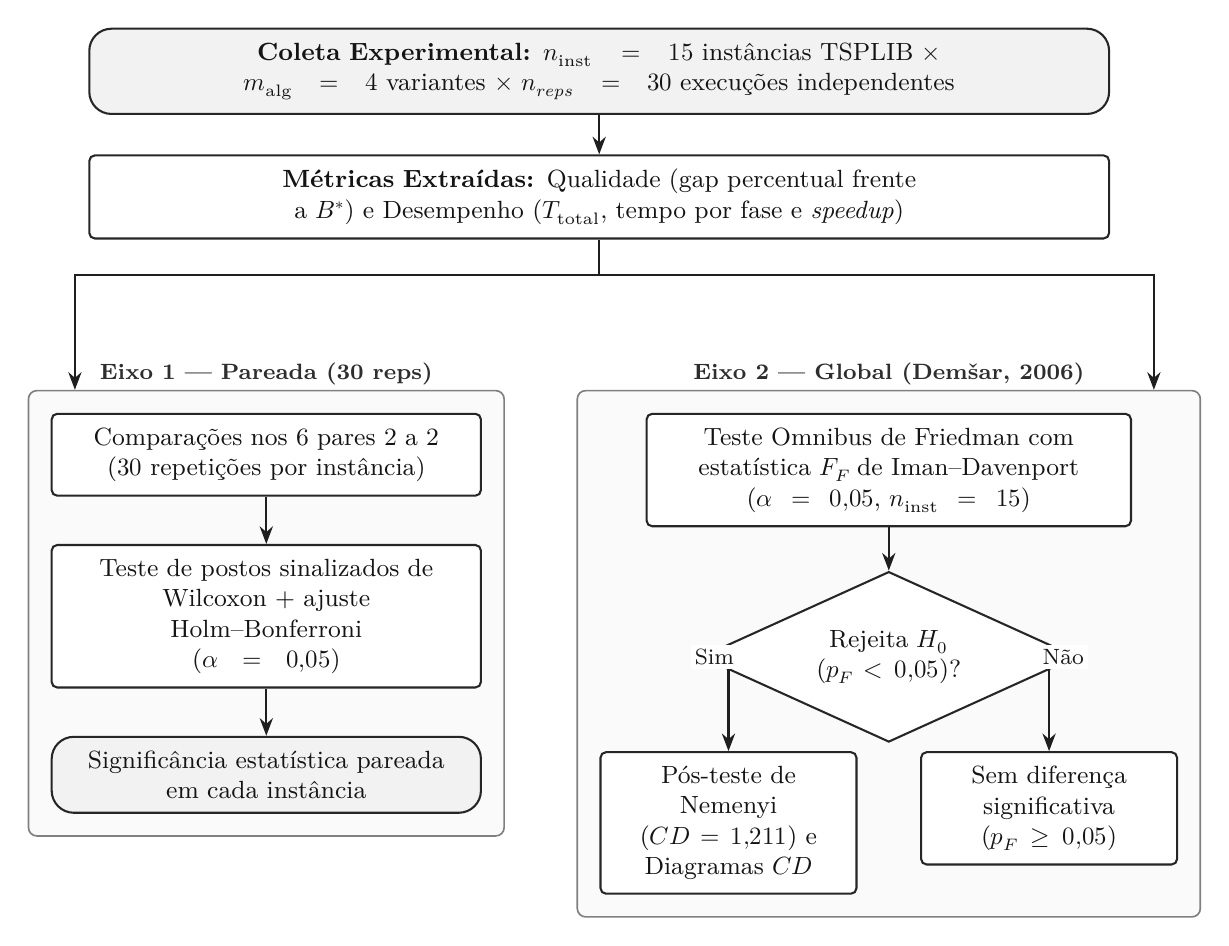
\begin{tikzpicture}[node distance=5.5mm and 8mm]
            % Topo comum
            \node[fc_term, text width=12.6cm] (collect) {\textbf{Coleta Experimental:} \(n_{\text{inst}} = \totalinstancias\) instâncias TSPLIB \(\times\) \(m_{\text{alg}} = \totalvariantes\) variantes \(\times\) \(n_{reps} = \totalrepeticoes\) execuções independentes};
            \node[fc_proc, below=5mm of collect, text width=12.6cm] (metrics) {\textbf{Métricas Extraídas:} Qualidade (\(\text{gap}\) percentual frente a \(B^*\)) e Desempenho (\(T_{\text{total}}\), tempo por fase e \emph{speedup})};

            % Eixo 1 (Esquerda): Analise Pareada
            \node[fc_proc, below left=22mm and -5.0cm of metrics, text width=5.1cm] (p1) {Comparações nos 6 pares 2 a 2\\(\(\totalrepeticoes\) repetições por instância)};
            \node[fc_proc, below=6mm of p1, text width=5.1cm] (p2) {Teste de postos sinalizados de\\Wilcoxon + ajuste Holm--Bonferroni\\(\(\alpha = 0{,}05\))};
            \node[fc_term, below=6mm of p2, text width=5.1cm] (p3) {Significância estatística pareada\\em cada instância};

            % Eixo 2 (Direita): Analise Global
            \node[fc_proc, below right=22mm and -5.9cm of metrics, text width=5.8cm] (g1) {Teste Omnibus de Friedman com\\ estatística \(F_F\) de Iman--Davenport\\(\(\alpha = 0{,}05\), \(n_{\text{inst}} = \totalinstancias\))};
            \node[fc_dec, below=5.5mm of g1, text width=2.7cm] (gdec) {Rejeita \(H_0\)\\(\(p_F < 0{,}05\))?};
            \node[fc_proc, below left=6.5mm and -0.8cm of gdec, text width=2.9cm] (gnem) {Pós-teste de Nemenyi\\(\(CD = 1{,}211\)) e\\Diagramas \(CD\)};
            \node[fc_proc, below right=6.5mm and -0.8cm of gdec, text width=2.9cm] (gno) {Sem diferença\\significativa\\(\(p_F \ge 0{,}05\))};

            % Caixas de fundo + títulos fc_grouptitle centralizados no topo com entrada simétrica deslocada da borda externa
            \begin{scope}[on background layer]
                  \node[fc_group, fit=(p1)(p2)(p3)] (box1) {};
                  \node[fc_group, fit=(g1)(gdec)(gnem)(gno)] (box2) {};
            \end{scope}
            \node[fc_grouptitle, fill=white, anchor=south] at (box1.north) {Eixo 1 — Pareada (\totalrepeticoes\ reps)};
            \node[fc_grouptitle, fill=white, anchor=south] at (box2.north) {Eixo 2 — Global (Demšar, 2006)};

            % Arestas ortogonais simétricas entrando nas bordas externas livres do titulo
            \draw[fc_arr] (collect) -- (metrics);
            \draw[fc_arr] (metrics.south) -- ++(0,-4.5mm) -| ($(box1.north west)+(0.6cm,0)$);
            \draw[fc_arr] (metrics.south) -- ++(0,-4.5mm) -| ($(box2.north east)+(-0.6cm,0)$);
            \draw[fc_arr] (p1) -- (p2);
            \draw[fc_arr] (p2) -- (p3);
            \draw[fc_arr] (g1) -- (gdec);
            \draw[fc_arr] (gdec) -| node[fc_lbl, pos=0.25] {Sim} (gnem);
            \draw[fc_arr] (gdec) -| node[fc_lbl, pos=0.25] {Não} (gno);
      \end{tikzpicture}
\end{figure}

\chapter{Resultados}\label{cap4-resultados}

Este capítulo apresenta os resultados experimentais obtidos a partir da execução das quatro variantes do algoritmo memético AG+\(2\)-opt (CPU, híbrida ingênua, híbrida otimizada e totalmente em GPU) sobre o conjunto completo de \totalinstancias\ instâncias da TSPLIB.
A análise é dividida em quatro partes principais:

\begin{enumerate}
  \item
        uma avaliação detalhada por instância, destacando a progressão entre \(\menorinstancia\) e \(\maiorinstancia\) cidades (com a tabela integral das \totalinstancias\ instâncias no \apref{apendice-resultados});
  \item
        uma análise agregada sobre todo o conjunto avaliado, focada nas métricas de performance e qualidade das soluções;
  \item
        a aplicação dos testes estatísticos não paramétricos descritos no \capref{cap3-materiais-metodos}, acompanhada dos diagramas de diferença crítica (tempo e \emph{gap}) e da análise de escalonamento; e
  \item
        a divisão do tempo de execução entre as oito etapas do ciclo evolutivo e a análise de gargalos com base na Lei de Amdahl.
\end{enumerate}

\section{Resultados experimentais}\label{sec-41-resultados-experimentais}

Os experimentos foram conduzidos conforme o protocolo definido na \secref{sec-33-selecao-instancias}, com \totalrepeticoes\ repetições independentes pareadas (sementes \(\sementeinicial\) a \(\sementefinal\)) para cada par algoritmo--instância, totalizando \(\totalcombinacoes\) combinações e \(\totalexecucoes\) execuções registradas.
Graças à busca local vetorizada associada à lista de candidatos \(k_{\text{viz}} = \kviz\), todas as quatro variantes foram executadas integralmente sobre todas as \totalinstancias\ instâncias selecionadas.

As métricas primárias coletadas foram:

\begin{itemize}
  \item
        \textbf{Tempo Médio de Execução (s):} Tempo total para completar a execução por repetição.
  \item
        \textbf{Gap Médio (\%):} Desvio percentual do custo da melhor solução encontrada em relação ao ótimo conhecido da instância.
  \item
        \textbf{Performance:} Razão entre o tempo de execução da variante de referência (CPU) e a variante avaliada.
\end{itemize}

\section{Análise por instância}\label{sec-42-analise-por-instancia}

A \tabref{tbl:results-detailed} reúne os resultados detalhados de sete instâncias selecionadas entre \(52\) e \(\maiorinstancia\) cidades (\texttt{berlin52}, \texttt{kroA100}, \texttt{d198}, \texttt{pr264}, \texttt{att532}, \texttt{si535} e \texttt{pr1002}); os valores completos de todas as \totalinstancias\ instâncias (de \(\menorinstancia\) a \(\maiorinstancia\) cidades) constam na \tabref{tbl:results-all-instances} do \apref{apendice-resultados}.

\begin{tabelapadrao}
  \begin{longtable}[]{@{}
      >{\raggedright\arraybackslash}p{(\linewidth - 12\tabcolsep) * \real{0.11}}
      >{\centering\arraybackslash}p{(\linewidth - 12\tabcolsep) * \real{0.07}}
      >{\raggedright\arraybackslash}p{(\linewidth - 12\tabcolsep) * \real{0.24}}
      >{\centering\arraybackslash}p{(\linewidth - 12\tabcolsep) * \real{0.26}}
      >{\centering\arraybackslash}p{(\linewidth - 12\tabcolsep) * \real{0.10}}
      >{\centering\arraybackslash}p{(\linewidth - 12\tabcolsep) * \real{0.11}}
      >{\centering\arraybackslash}p{(\linewidth - 12\tabcolsep) * \real{0.11}}@{}}
    \caption{Resultados detalhados por instância (seleção representativa)}\label{tbl:results-detailed}                                                   \\
    \toprule
    Instância         & \(n_{coords}\) & Algoritmo         & Custo médio (\(\pm \sigma\))  & \emph{Gap} médio (\%) & Tempo médio (s) & Ganho de perf.    \\
    \midrule
    \endfirsthead
    \toprule
    Instância         & \(n_{coords}\) & Algoritmo         & Custo médio (\(\pm \sigma\))  & \emph{Gap} médio (\%) & Tempo médio (s) & Ganho de perf.    \\
    \midrule
    \endhead
    \bottomrule
    \endlastfoot
    \textbf{berlin52} & 52             & CPU               & \(7553{,}03 \pm 17{,}39\)     & \(0{,}15\)            & \(1{,}59\)      & \(1{,}00\times\)  \\*
                      & 52             & Híbrida Ingênua   & \(7545{,}23 \pm 12{,}25\)     & \(0{,}04\)            & \(0{,}51\)      & \(3{,}12\times\)  \\*
                      & 52             & Híbrida Otimizada & \(7545{,}23 \pm 12{,}25\)     & \(0{,}04\)            & \(0{,}08\)      & \(20{,}23\times\) \\*
                      & 52             & Totalmente em GPU & \(7550{,}97 \pm 19{,}97\)     & \(0{,}12\)            & \(0{,}02\)      & \(75{,}03\times\) \\
    \midrule
    \textbf{kroA100}  & 100            & CPU               & \(21389{,}43 \pm 54{,}23\)    & \(0{,}50\)            & \(4{,}81\)      & \(1{,}00\times\)  \\*
                      & 100            & Híbrida Ingênua   & \(21391{,}40 \pm 63{,}09\)    & \(0{,}51\)            & \(1{,}18\)      & \(4{,}06\times\)  \\*
                      & 100            & Híbrida Otimizada & \(21391{,}40 \pm 63{,}09\)    & \(0{,}51\)            & \(0{,}19\)      & \(25{,}73\times\) \\*
                      & 100            & Totalmente em GPU & \(21372{,}60 \pm 56{,}96\)    & \(0{,}43\)            & \(0{,}05\)      & \(94{,}86\times\) \\
    \midrule
    \textbf{d198}     & 198            & CPU               & \(15918{,}27 \pm 16{,}32\)    & \(0{,}88\)            & \(14{,}66\)     & \(1{,}00\times\)  \\*
                      & 198            & Híbrida Ingênua   & \(15916{,}07 \pm 14{,}70\)    & \(0{,}86\)            & \(3{,}08\)      & \(4{,}76\times\)  \\*
                      & 198            & Híbrida Otimizada & \(15916{,}07 \pm 14{,}70\)    & \(0{,}86\)            & \(0{,}55\)      & \(26{,}84\times\) \\*
                      & 198            & Totalmente em GPU & \(15912{,}93 \pm 18{,}04\)    & \(0{,}84\)            & \(0{,}17\)      & \(88{,}62\times\) \\
    \midrule
    \textbf{pr264}    & 264            & CPU               & \(49552{,}43 \pm 71{,}20\)    & \(0{,}85\)            & \(23{,}62\)     & \(1{,}00\times\)  \\*
                      & 264            & Híbrida Ingênua   & \(49551{,}47 \pm 98{,}13\)    & \(0{,}85\)            & \(4{,}81\)      & \(4{,}91\times\)  \\*
                      & 264            & Híbrida Otimizada & \(49551{,}47 \pm 98{,}13\)    & \(0{,}85\)            & \(1{,}02\)      & \(23{,}15\times\) \\*
                      & 264            & Totalmente em GPU & \(49527{,}90 \pm 80{,}20\)    & \(0{,}80\)            & \(0{,}34\)      & \(69{,}92\times\) \\
    \midrule
    \textbf{att532}   & 532            & CPU               & \(28000{,}10 \pm 83{,}69\)    & \(1{,}13\)            & \(158{,}24\)    & \(1{,}00\times\)  \\*
                      & 532            & Híbrida Ingênua   & \(27981{,}53 \pm 57{,}22\)    & \(1{,}07\)            & \(29{,}33\)     & \(5{,}39\times\)  \\*
                      & 532            & Híbrida Otimizada & \(27981{,}53 \pm 57{,}22\)    & \(1{,}07\)            & \(6{,}67\)      & \(23{,}73\times\) \\*
                      & 532            & Totalmente em GPU & \(27999{,}93 \pm 78{,}55\)    & \(1{,}13\)            & \(3{,}39\)      & \(46{,}63\times\) \\
    \midrule
    \textbf{si535}    & 535            & CPU               & \(48903{,}20 \pm 21{,}15\)    & \(0{,}94\)            & \(84{,}19\)     & \(1{,}00\times\)  \\*
                      & 535            & Híbrida Ingênua   & \(48900{,}00 \pm 23{,}95\)    & \(0{,}93\)            & \(10{,}97\)     & \(7{,}68\times\)  \\*
                      & 535            & Híbrida Otimizada & \(48900{,}00 \pm 23{,}95\)    & \(0{,}93\)            & \(2{,}48\)      & \(33{,}99\times\) \\*
                      & 535            & Totalmente em GPU & \(48909{,}00 \pm 18{,}43\)    & \(0{,}95\)            & \(1{,}23\)      & \(68{,}23\times\) \\
    \midrule
    \textbf{pr1002}   & 1002           & CPU               & \(263558{,}83 \pm 771{,}47\)  & \(1{,}74\)            & \(682{,}58\)    & \(1{,}00\times\)  \\*
                      & 1002           & Híbrida Ingênua   & \(263288{,}90 \pm 954{,}07\)  & \(1{,}64\)            & \(115{,}35\)    & \(5{,}92\times\)  \\*
                      & 1002           & Híbrida Otimizada & \(263288{,}90 \pm 954{,}07\)  & \(1{,}64\)            & \(25{,}55\)     & \(26{,}72\times\) \\*
                      & 1002           & Totalmente em GPU & \(263409{,}57 \pm 1121{,}29\) & \(1{,}68\)            & \(14{,}03\)     & \(48{,}66\times\) \\
  \end{longtable}
  \notatabela{Médias sobre as \totalrepeticoes\ repetições. Os ganhos de velocidade (\textit{Ganho de perf.}) foram calculados a partir dos tempos médios exatos antes do arredondamento a duas casas decimais (por exemplo, em \texttt{berlin52}, \(1{,}594134\,\text{s} / 0{,}021246\,\text{s} \approx 75{,}03\times\)).}
\end{tabelapadrao}

Nas instâncias menores e intermediárias da tabela (\texttt{berlin52}, \texttt{kroA100} e \texttt{d198}), a variante \textbf{Totalmente em GPU} atinge os maiores ganhos relativos sobre a CPU: \(94{,}86\times\) em \texttt{kroA100} (\(0{,}05\)\,s contra \(4{,}81\)\,s), \(88{,}62\times\) em \texttt{d198} (\(0{,}17\)\,s contra \(14{,}66\)\,s) e \(75{,}03\times\) em \texttt{berlin52} (\(0{,}02\)\,s contra \(1{,}59\)\,s) --- chegando a \(112{,}48\times\) em \texttt{gr96} na tabela integral do \apref{apendice-resultados}.
A \textbf{Híbrida Otimizada} ocupa consistentemente o segundo lugar (\(20{,}23\times\) a \(26{,}84\times\) nessas três instâncias), muito à frente da \textbf{Híbrida Ingênua} (\(3{,}12\times\) a \(4{,}76\times\)).

Em \texttt{pr264} (\(264\) cidades), a mesma hierarquia se mantém: a \textbf{Totalmente em GPU} conclui em \(0{,}34\)\,s (\(69{,}92\times\) mais rápida que a CPU), seguida pela \textbf{Híbrida Otimizada} (\(1{,}02\)\,s; \(23{,}15\times\)) e pela \textbf{Híbrida Ingênua} (\(4{,}81\)\,s; \(4{,}91\times\)).
Avançando para \texttt{att532} (\(532\)), \texttt{si535} (\(535\)) e \texttt{pr1002} (\(\maiorinstancia\)), o ganho em tempo absoluto fica ainda mais evidente: em \texttt{pr1002}, a \textbf{Totalmente em GPU} reduz o tempo médio de \(682{,}58\)\,s na CPU para \(14{,}03\)\,s (\(48{,}66\times\) mais rápida que a CPU, \(8{,}22\times\) que a Híbrida Ingênua com \(115{,}35\)\,s e \(1{,}82\times\) que a Híbrida Otimizada com \(25{,}55\)\,s).
Em relação à qualidade das soluções, os \emph{gaps} permanecem praticamente iguais entre as variantes ao longo de toda a tabela --- em \texttt{pr1002}, por exemplo, eles ficam em \(1{,}74\%\) na CPU, \(1{,}64\%\) nas duas variantes híbridas (idênticas bit a bit nas \totalrepeticoes\ sementes) e \(1{,}68\%\) na Totalmente em GPU.

\section{Análise agregada, testes estatísticos e escalonamento}\label{sec-43-analise-agregada}

Ao agregar os resultados de todas as \totalinstancias\ instâncias, emergem padrões claros de desempenho que caracterizam o comportamento temporal e a qualidade das soluções.

\begin{tabelapadrao}
  \begin{longtable}[]{@{}
      >{\raggedright\arraybackslash}p{(\linewidth - 6\tabcolsep) * \real{0.25}}
      >{\centering\arraybackslash}p{(\linewidth - 6\tabcolsep) * \real{0.31}}
      >{\centering\arraybackslash}p{(\linewidth - 6\tabcolsep) * \real{0.22}}
      >{\centering\arraybackslash}p{(\linewidth - 6\tabcolsep) * \real{0.22}}@{}}
    \caption{Desempenho agregado sobre todas as \totalinstancias\ instâncias}\label{tbl:results-aggregated}           \\
    \toprule
    Algoritmo         & Tempo mediano \([Q_{25};\, Q_{75}]\) (s) & \emph{Gap} médio (\%) & Ganho rel. CPU (geom.)     \\
    \midrule
    \endfirsthead
    \toprule
    Algoritmo         & Tempo mediano \([Q_{25};\, Q_{75}]\) (s) & \emph{Gap} médio (\%) & Ganho rel. CPU (geom.)     \\
    \midrule
    \endhead
    \bottomrule
    \endlastfoot
    CPU               & \(23{,}62\;[4{,}81;\, 130{,}73]\)        & \(0{,}90 \pm 0{,}41\) & \(1{,}00\times\)           \\
    Híbrida Ingênua   & \(4{,}81\;[1{,}17;\, 25{,}76]\)          & \(0{,}90 \pm 0{,}44\) & \(4{,}57\times\)           \\
    Híbrida Otimizada & \(1{,}02\;[0{,}18;\, 6{,}02]\)           & \(0{,}90 \pm 0{,}44\) & \(23{,}86\times\)          \\
    Totalmente em GPU & \(\mathbf{0{,}34\;[0{,}05;\, 2{,}72]}\)  & \(0{,}91 \pm 0{,}46\) & \(\mathbf{71{,}03\times}\) \\
  \end{longtable}
  \notatabela{Como os tempos de execução variam em ordens de grandeza entre \(n_{coords} = \menorinstancia\) e \(\maiorinstancia\), o tempo agregado é resumido por mediana e intervalo interquartil (\([Q_{25};\, Q_{75}]\)), evitando a distorção de médias aritméticas sobre amostras fortemente assimétricas; o ganho relativo à CPU utiliza a média geométrica das \totalinstancias\ razões por instância.}
\end{tabelapadrao}

A \tabref{tbl:results-aggregated} resume duas conclusões centrais sobre o comportamento empírico do algoritmo memético:

\begin{enumerate}
  \item
        \textbf{A variante Totalmente em GPU obtém o menor tempo de execução:} Com ganho médio geométrico de \(71{,}03\times\) sobre a CPU, \(15{,}53\times\) sobre a Híbrida Ingênua e \(2{,}98\times\) sobre a Híbrida Otimizada (tempo mediano de \(0{,}34\)\,s com IIQ \([0{,}05;\, 2{,}72]\)\,s contra \(23{,}62\)\,s e IIQ \([4{,}81;\, 130{,}73]\)\,s na CPU), a versão residente em GPU confirma que manter a população, os operadores evolutivos e a busca local na VRAM traz três benefícios combinados: elimina o tráfego de matrizes de rotas pelo barramento PCIe a cada geração, evita lançamentos individuais de \emph{kernels} e remove o gargalo dos operadores executados em CPU (sobretudo o cruzamento, detalhado na \secref{sec-44-decomposicao-fases}).
        A Híbrida Otimizada fica em segundo lugar, com ganho geométrico de \(23{,}86\times\) sobre a CPU e \(5{,}22\times\) sobre a Híbrida Ingênua (mediana de \(1{,}02\)\,s contra \(4{,}81\)\,s da Híbrida Ingênua, que atinge \(4{,}57\times\) sobre a CPU).
  \item
        \textbf{Qualidade das soluções preservada entre arquiteturas:} Com os mesmos parâmetros de busca local (\(\kappa = \maxpassadas\) varreduras e \(k_{\text{viz}} = \kviz\) candidatos), as quatro variantes atingem soluções com qualidade muito próxima: os \emph{gaps} médios agregados ficam em \(0{,}90\% \pm 0{,}41\%\) na CPU, \(0{,}90\% \pm 0{,}44\%\) nas duas variantes híbridas e \(0{,}91\% \pm 0{,}46\%\) na Totalmente em GPU.
\end{enumerate}

Para confirmar estatisticamente essas duas conclusões, aplicaram-se o Eixo~1 (\secref{sec-341-eixo1}) e o Eixo~2 (\secref{sec-342-eixo2}) do protocolo de \textcite{demsar2006statistical} ao nível \(\alpha = 0{,}05\):

\begin{itemize}
  \item
        \textbf{Qualidade das soluções (\emph{gap} percentual):} Não há diferença estatisticamente significativa entre as quatro variantes em nenhum dos dois eixos. No Eixo~2 global, o teste de Friedman com correção de Iman--Davenport não rejeita \(H_0\) (\(\chi_F^2 = 2{,}69\); \(F_F(3, 42) = 0{,}8897\); \(p = 0{,}4543 > 0{,}05\)), os postos médios ficam muito próximos (\(2{,}30\) nas duas híbridas, \(2{,}47\) na Totalmente em GPU e \(2{,}93\) na CPU), nenhum par supera \(CD = 1{,}211\) (\figref{fig:cd-diagram-gap}) e os contrastes contra a CPU resultam em \(p_{\text{Holm}} = 1{,}00\). No Eixo~1 por instância (\tabref{tbl:axis1-wilcoxon} do \apref{apendice-resultados}), \(0\) das \(90\) comparações pareadas (\(6\) pares \(\times\) \(\totalinstancias\) instâncias) são significativas (\(p_{\text{Holm}} \ge 0{,}3418\)), com diferenças exatamente nulas entre as duas híbridas em todas as sementes (identidade bit a bit).
  \item
        \textbf{Tempo de execução:} A superioridade temporal das variantes aceleradas é confirmada em ambos os eixos. No Eixo~2 global, a ordenação foi idêntica nas \totalinstancias\ instâncias (\(\chi_F^2 = 45{,}00\), \(p < 0{,}001\); postos médios exatos \(1{,}00\), \(2{,}00\), \(3{,}00\) e \(4{,}00\)), todas as variantes em GPU superam a CPU via Wilcoxon com Holm--Bonferroni (\(p_{\text{Holm}} < 0{,}001\)) e o pós-teste de Nemenyi (\figref{fig:cd-diagram-time}, \(CD = 1{,}211\)) separa todos os pares distantes por duas ou mais posições (pares vizinhos ficam à distância \(1{,}00 < 1{,}211\)). No Eixo~1 por instância (\tabref{tbl:axis1-wilcoxon}), todos os \(6\) pares possíveis entre as \totalvariantes\ variantes diferem em todas as \totalinstancias\ instâncias (\(90/90\) testes com \(p_{\text{Holm}} \le 2{,}05 \times 10^{-7}\)), confirmando também a vantagem da Totalmente em GPU sobre a Híbrida Otimizada em cada instância individualmente.
\end{itemize}

\begin{figure}[htbp]
  \centering
  \caption{Diagrama de diferença crítica de Demšar (pós-teste de Nemenyi, \(CD = 1{,}211\), \(\alpha = 0{,}05\)) para o \textbf{tempo de execução} nas \totalinstancias\ instâncias: ordenação idêntica em todas elas (\(\chi_F^2 = 45{,}00\), \(p < 0{,}001\))}\label{fig:cd-diagram-time}
  \begin{adjustbox}{max width=\linewidth}
    % Auto-generated Demšar Critical Difference Diagram in TikZ
% Metric: Tempo de Execução
% Generated for k = 4 algorithms across N = 15 instances (CD = 1.211, alpha = 0.05, F_F = inf, p = 0)
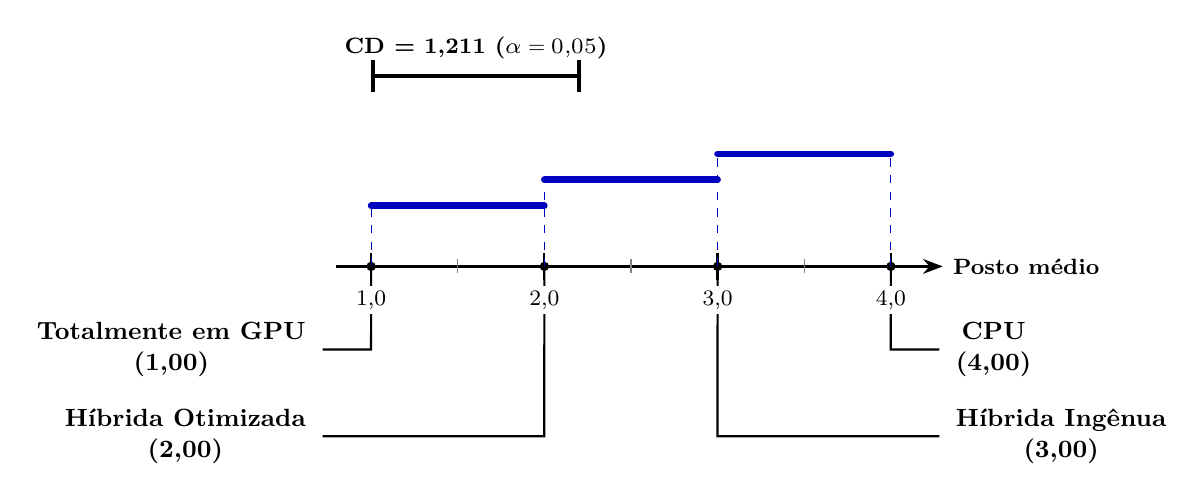
\begin{tikzpicture}[
    scale=2.2,
    axis/.style={thick, -{Stealth[length=2.5mm]}},
    tick/.style={thick},
    subtick/.style={thin, gray},
    clique/.style={line width=2.4pt, color=blue!75!black, line cap=round},
    cdbar/.style={line width=1.5pt, {Bar[width=4mm]}-{Bar[width=4mm]}},
    algomarker/.style={circle, fill=black, inner sep=1.2pt},
    labelnode/.style={font=\small\bfseries, align=center}
]

    % 1. CD Reference Bar at the Top
    \draw[cdbar] (1.0, 1.10) -- node[above=2pt, font=\footnotesize\bfseries] {CD = 1,211 ($\alpha = 0{,}05$)} (2.211, 1.10);

    % 2. Main Horizontal Rank Axis (1.0 to k.0)
    \draw[axis] (0.8, 0.0) -- (4.3, 0.0) node[right, font=\footnotesize\bfseries] {Posto médio};

    % Major Ticks
    \draw[tick] (1.0, 0.08) -- (1.0, -0.08);
    \draw[tick] (2.0, 0.08) -- (2.0, -0.08);
    \draw[tick] (3.0, 0.08) -- (3.0, -0.08);
    \draw[tick] (4.0, 0.08) -- (4.0, -0.08);

    % Minor Sub-ticks (every 0.5)
    \draw[subtick] (1.5, 0.04) -- (1.5, -0.04);
    \draw[subtick] (2.5, 0.04) -- (2.5, -0.04);
    \draw[subtick] (3.5, 0.04) -- (3.5, -0.04);

    % 3. Algorithm Data Points and Drop Lines (staggered Demšar elbows avoid overlap on ties)
    \coordinate (A_FullGPUModular) at (1.000, 0.0);
    \node[algomarker] at (A_FullGPUModular) {};
    \draw[thick] (A_FullGPUModular) -- (1.000, -0.48) -- (0.72, -0.48);
    \node[labelnode, anchor=east] at (0.68, -0.48) {Totalmente em GPU\\(1,00)};
    \coordinate (A_HybridOptimized) at (2.000, 0.0);
    \node[algomarker] at (A_HybridOptimized) {};
    \draw[thick] (A_HybridOptimized) -- (2.000, -0.98) -- (0.72, -0.98);
    \node[labelnode, anchor=east] at (0.68, -0.98) {Híbrida Otimizada\\(2,00)};
    \coordinate (A_HybridNaive) at (3.000, 0.0);
    \node[algomarker] at (A_HybridNaive) {};
    \draw[thick] (A_HybridNaive) -- (3.000, -0.98) -- (4.28, -0.98);
    \node[labelnode, anchor=west] at (4.32, -0.98) {Híbrida Ingênua\\(3,00)};
    \coordinate (A_CPU) at (4.000, 0.0);
    \node[algomarker] at (A_CPU) {};
    \draw[thick] (A_CPU) -- (4.000, -0.48) -- (4.28, -0.48);
    \node[labelnode, anchor=west] at (4.32, -0.48) {CPU\\(4,00)};

    % Major Tick Labels (drawn after drop lines so white fill masks crossings)
    \node[below=2pt, font=\footnotesize, fill=white, inner sep=1.5pt] at (1.0, -0.08) {1,0};
    \node[below=2pt, font=\footnotesize, fill=white, inner sep=1.5pt] at (2.0, -0.08) {2,0};
    \node[below=2pt, font=\footnotesize, fill=white, inner sep=1.5pt] at (3.0, -0.08) {3,0};
    \node[below=2pt, font=\footnotesize, fill=white, inner sep=1.5pt] at (4.0, -0.08) {4,0};

    % 4. Non-Significant Cliques (|R_i - R_j| <= CD)
    \draw[clique] (1.000, 0.35) -- (2.000, 0.35);
    \draw[thin, blue!75!black, dashed] (1.000, 0.0) -- (1.000, 0.35);
    \draw[thin, blue!75!black, dashed] (2.000, 0.0) -- (2.000, 0.35);
    \draw[clique] (2.000, 0.50) -- (3.000, 0.50);
    \draw[thin, blue!75!black, dashed] (2.000, 0.0) -- (2.000, 0.50);
    \draw[thin, blue!75!black, dashed] (3.000, 0.0) -- (3.000, 0.50);
    \draw[clique] (3.000, 0.65) -- (4.000, 0.65);
    \draw[thin, blue!75!black, dashed] (3.000, 0.0) -- (3.000, 0.65);
    \draw[thin, blue!75!black, dashed] (4.000, 0.0) -- (4.000, 0.65);
\end{tikzpicture}

  \end{adjustbox}
\end{figure}

\begin{figure}[htbp]
  \centering
  \caption{Diagrama de diferença crítica de Demšar (pós-teste de Nemenyi, \(CD = 1{,}211\), \(\alpha = 0{,}05\)) para a \textbf{qualidade da solução (\emph{gap} percentual)}: nenhum par apresenta diferença estatisticamente significativa (\(\chi_F^2 = 2{,}69\), \(F_F(3, 42) = 0{,}8897\), \(p = 0{,}4543\))}\label{fig:cd-diagram-gap}
  \begin{adjustbox}{max width=\linewidth}
    % Auto-generated Demšar Critical Difference Diagram in TikZ
% Metric: Gap de Otimalidade
% Generated for k = 4 algorithms across N = 15 instances (CD = 1.211, alpha = 0.05, F_F = 0.890, p = 0.4543)
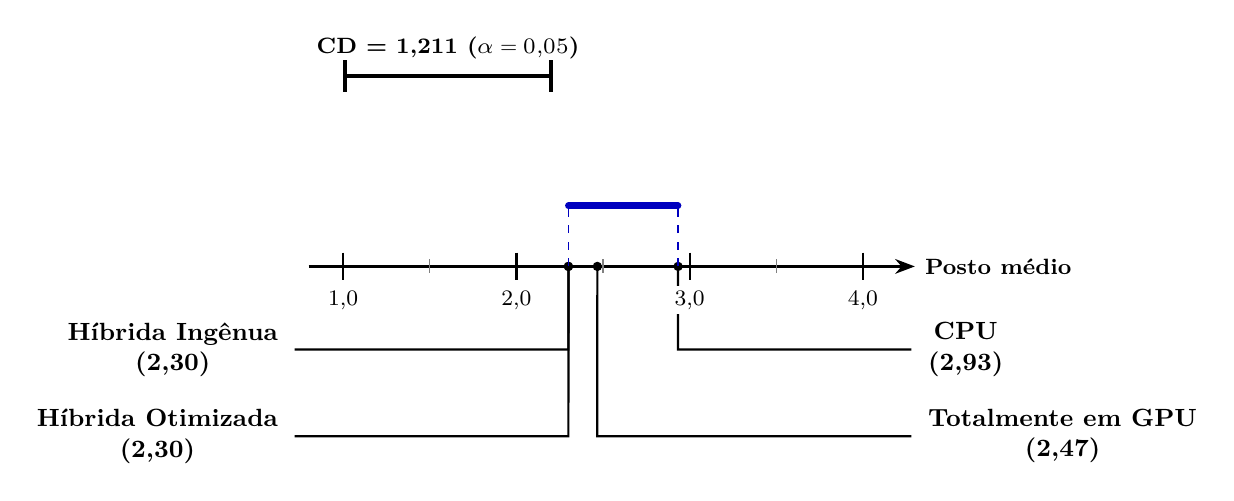
\begin{tikzpicture}[
    scale=2.2,
    axis/.style={thick, -{Stealth[length=2.5mm]}},
    tick/.style={thick},
    subtick/.style={thin, gray},
    clique/.style={line width=2.4pt, color=blue!75!black, line cap=round},
    cdbar/.style={line width=1.5pt, {Bar[width=4mm]}-{Bar[width=4mm]}},
    algomarker/.style={circle, fill=black, inner sep=1.2pt},
    labelnode/.style={font=\small\bfseries, align=center}
]

    % 1. CD Reference Bar at the Top
    \draw[cdbar] (1.0, 1.10) -- node[above=2pt, font=\footnotesize\bfseries] {CD = 1,211 ($\alpha = 0{,}05$)} (2.211, 1.10);

    % 2. Main Horizontal Rank Axis (1.0 to k.0)
    \draw[axis] (0.8, 0.0) -- (4.3, 0.0) node[right, font=\footnotesize\bfseries] {Posto médio};

    % Major Ticks
    \draw[tick] (1.0, 0.08) -- (1.0, -0.08);
    \draw[tick] (2.0, 0.08) -- (2.0, -0.08);
    \draw[tick] (3.0, 0.08) -- (3.0, -0.08);
    \draw[tick] (4.0, 0.08) -- (4.0, -0.08);

    % Minor Sub-ticks (every 0.5)
    \draw[subtick] (1.5, 0.04) -- (1.5, -0.04);
    \draw[subtick] (2.5, 0.04) -- (2.5, -0.04);
    \draw[subtick] (3.5, 0.04) -- (3.5, -0.04);

    % 3. Algorithm Data Points and Drop Lines (staggered Demšar elbows avoid overlap on ties)
    \coordinate (A_HybridNaive) at (2.300, 0.0);
    \node[algomarker] at (A_HybridNaive) {};
    \draw[thick] (A_HybridNaive) -- (2.300, -0.48) -- (0.72, -0.48);
    \node[labelnode, anchor=east] at (0.68, -0.48) {Híbrida Ingênua\\(2,30)};
    \coordinate (A_HybridOptimized) at (2.300, 0.0);
    \node[algomarker] at (A_HybridOptimized) {};
    \draw[thick] (A_HybridOptimized) -- (2.300, -0.98) -- (0.72, -0.98);
    \node[labelnode, anchor=east] at (0.68, -0.98) {Híbrida Otimizada\\(2,30)};
    \coordinate (A_FullGPUModular) at (2.467, 0.0);
    \node[algomarker] at (A_FullGPUModular) {};
    \draw[thick] (A_FullGPUModular) -- (2.467, -0.98) -- (4.28, -0.98);
    \node[labelnode, anchor=west] at (4.32, -0.98) {Totalmente em GPU\\(2,47)};
    \coordinate (A_CPU) at (2.933, 0.0);
    \node[algomarker] at (A_CPU) {};
    \draw[thick] (A_CPU) -- (2.933, -0.48) -- (4.28, -0.48);
    \node[labelnode, anchor=west] at (4.32, -0.48) {CPU\\(2,93)};

    % Major Tick Labels (drawn after drop lines so white fill masks crossings)
    \node[below=2pt, font=\footnotesize, fill=white, inner sep=1.5pt] at (1.0, -0.08) {1,0};
    \node[below=2pt, font=\footnotesize, fill=white, inner sep=1.5pt] at (2.0, -0.08) {2,0};
    \node[below=2pt, font=\footnotesize, fill=white, inner sep=1.5pt] at (3.0, -0.08) {3,0};
    \node[below=2pt, font=\footnotesize, fill=white, inner sep=1.5pt] at (4.0, -0.08) {4,0};

    % 4. Non-Significant Cliques (|R_i - R_j| <= CD)
    \draw[clique] (2.300, 0.35) -- (2.933, 0.35);
    \draw[thin, blue!75!black, dashed] (2.300, 0.0) -- (2.300, 0.35);
    \draw[thin, blue!75!black, dashed] (2.933, 0.0) -- (2.933, 0.35);
\end{tikzpicture}

  \end{adjustbox}
\end{figure}

A \figref{fig:scaling-time-gap} mostra como o tempo total de execução até o critério de parada (em escala logarítmica, painel superior) e o \emph{gap} percentual (painel inferior) evoluem conforme o número de cidades \(n\) cresce até \(\maiorinstancia\).
Para cada instância, as curvas representam a mediana das \totalrepeticoes\ repetições e as faixas sombreadas indicam o intervalo onde ficam os \(50\%\) centrais das execuções (\(Q_{25}\text{--}Q_{75}\)), evitando possíveis distorções causadas por execuções fora do padrão.
O gráfico confirma visualmente os dois resultados principais: uma separação consistente em ordens de grandeza no tempo entre as variantes e curvas de \emph{gap} praticamente sobrepostas.

\begin{figure}[htbp]
  \centering
  \caption{Evolução do tempo total de execução até a parada (escala logarítmica, painel superior) e do \emph{gap} percentual em relação ao ótimo da TSPLIB (painel inferior) conforme o número de cidades \(n\), exibindo a mediana e o intervalo dos \(50\%\) centrais (\(Q_{25}\text{--}Q_{75}\)) nas \totalrepeticoes\ repetições}\label{fig:scaling-time-gap}
  \includegraphics[width=\linewidth]{../../../benchmark_scripts/experiments-and-examples/chapter4/results/figures/scaling_time_gap.pdf}
\end{figure}

Dois comportamentos pontuais na \figref{fig:scaling-time-gap} decorrem diretamente do critério de parada (\(\varepsilon_{\text{alvo}} = 1\%\)) e da dificuldade própria de cada instância:

\begin{itemize}
  \item
        \textbf{Queda de \emph{gap} em \texttt{berlin52} e tempos curtos abaixo de \(100\) cidades:} Enquanto \texttt{att48} e \texttt{eil51} encerram na maioria das vezes assim que cruzam a tolerância \(\varepsilon_{\text{alvo}} = 1\%\) (\(106\) e \(116\) de \(\totalexecinstancia\) execuções, respectivamente), em \texttt{berlin52} a busca atinge o ótimo exato (\(\text{gap} = 0\%\)) em \(95\) de \(\totalexecinstancia\) execuções (em menos de \(5\) gerações em média), derrubando a mediana para perto de zero. Nessas instâncias pequenas, a variante Totalmente em GPU conclui em menos de \(100\)\,ms (\(14{,}0\)\,ms em \texttt{att48} a \(42{,}7\)\,ms em \texttt{gr96}), faixa em que o custo fixo de lançamento e sincronização de \emph{kernels} tem peso proporcional maior.
  \item
        \textbf{Redução de tempo entre \texttt{att532} (\(n = 532\)) e \texttt{si535} (\(n = 535\)):} Embora cada geração individual de \texttt{si535} leve ligeiramente mais tempo que em \texttt{att532}, todas as \(\totalexecinstancia\) execuções de \texttt{si535} atingem \(\varepsilon_{\text{alvo}} = 1\%\) em cerca de \(63\) gerações, contra \(173\) a \(194\) gerações em \texttt{att532} (onde \(47\) de \(\totalexecinstancia\) execuções encerram por estagnação acima de \(1\%\)). Como o gráfico plota o tempo total até a parada, esse menor número de gerações reduz o tempo total em \(46{,}8\%\) na CPU e em cerca de \(63\%\) nas GPUs --- e, pela proximidade entre \(n = 532\) e \(n = 535\) no eixo linear contínuo, a transição entre os dois pontos aparece como um degrau quase vertical.
\end{itemize}

\section{Divisão do tempo por etapa e análise de gargalos}\label{sec-44-decomposicao-fases}

Para explicar as diferenças de desempenho entre as arquiteturas sem depender apenas do tempo total, a \tabref{tbl:phase-timings} mostra a participação percentual de cada uma das oito etapas do ciclo evolutivo (\secref{apendice-telemetria}). Os valores de todas as \totalinstancias\ instâncias constam na \tabref{tbl:phase-timings-all} do \apref{apendice-resultados}.

\begin{table}[htbp]
  \centering
  \caption{Divisão percentual do tempo médio de execução entre as oito etapas do ciclo evolutivo (instâncias selecionadas)}\label{tbl:phase-timings}
  \begin{tabeladensa}
    \begin{tabular}{@{}llrccccccccc@{}}
      \toprule
      Instância         & Algoritmo         & Tempo (ms) & Inic. & Sel. & Cruz. & Mut. & Aval. & BL   & Sobr. & Sinc. & Total \\
      \midrule
      \textbf{berlin52} & CPU               & 1594,1     & 0,1   & 0,0  & 3,2   & 0,0  & 0,0   & 96,5 & 0,0   & 0,0   & 100,0 \\
                        & Híbrida Ingênua   & 510,7      & 0,2   & 0,1  & 10,5  & 0,1  & 0,2   & 88,7 & 0,1   & 0,0   & 99,9  \\
                        & Híbrida Otimizada & 78,8       & 2,2   & 0,6  & 79,0  & 0,9  & 2,3   & 13,8 & 0,6   & 0,2   & 99,6  \\
                        & Totalmente em GPU & 21,2       & 8,8   & 8,0  & 8,7   & 9,9  & 5,4   & 8,7  & 13,0  & 36,0  & 98,4  \\
      \midrule
      \textbf{kroA100}  & CPU               & 4805,8     & 0,0   & 0,0  & 2,5   & 0,0  & 0,0   & 97,3 & 0,0   & 0,0   & 100,0 \\
                        & Híbrida Ingênua   & 1183,2     & 0,1   & 0,1  & 10,7  & 0,1  & 0,2   & 88,6 & 0,1   & 0,0   & 100,0 \\
                        & Híbrida Otimizada & 186,8      & 1,1   & 0,6  & 73,1  & 0,8  & 1,8   & 21,6 & 0,6   & 0,2   & 99,7  \\
                        & Totalmente em GPU & 50,7       & 3,6   & 5,6  & 6,1   & 7,3  & 3,6   & 6,0  & 7,7   & 59,0  & 99,0  \\
      \midrule
      \textbf{d198}     & CPU               & 14658,7    & 0,0   & 0,0  & 2,0   & 0,0  & 0,0   & 97,9 & 0,0   & 0,0   & 100,0 \\
                        & Híbrida Ingênua   & 3079,6     & 0,1   & 0,1  & 12,0  & 0,1  & 0,3   & 87,2 & 0,1   & 0,0   & 100,0 \\
                        & Híbrida Otimizada & 546,1      & 0,5   & 0,5  & 63,7  & 0,7  & 1,4   & 32,0 & 0,7   & 0,1   & 99,7  \\
                        & Totalmente em GPU & 165,4      & 1,1   & 2,7  & 3,1   & 3,8  & 1,2   & 3,3  & 4,1   & 80,1  & 99,5  \\
      \midrule
      \textbf{pr264}    & CPU               & 23616,8    & 0,0   & 0,0  & 1,8   & 0,0  & 0,1   & 98,1 & 0,0   & 0,0   & 100,0 \\
                        & Híbrida Ingênua   & 4813,3     & 0,1   & 0,1  & 14,4  & 0,2  & 0,4   & 84,6 & 0,1   & 0,0   & 100,0 \\
                        & Híbrida Otimizada & 1020,2     & 0,4   & 0,5  & 60,9  & 0,7  & 1,3   & 35,3 & 0,7   & 0,1   & 99,8  \\
                        & Totalmente em GPU & 337,7      & 0,7   & 2,1  & 2,5   & 3,0  & 0,9   & 2,6  & 3,2   & 84,7  & 99,7  \\
      \midrule
      \textbf{att532}   & CPU               & 158238,2   & 0,0   & 0,0  & 1,7   & 0,0  & 0,1   & 98,2 & 0,0   & 0,0   & 100,0 \\
                        & Híbrida Ingênua   & 29333,2    & 0,0   & 0,1  & 10,9  & 0,1  & 0,5   & 88,1 & 0,1   & 0,0   & 100,0 \\
                        & Híbrida Otimizada & 6667,0     & 0,1   & 0,5  & 52,5  & 0,6  & 1,0   & 44,4 & 0,7   & 0,1   & 99,8  \\
                        & Totalmente em GPU & 3393,2     & 0,1   & 1,5  & 1,5   & 1,8  & 0,5   & 1,4  & 2,0   & 91,1  & 99,8  \\
      \midrule
      \textbf{si535}    & CPU               & 84187,4    & 0,0   & 0,0  & 1,2   & 0,0  & 0,1   & 98,7 & 0,0   & 0,0   & 100,0 \\
                        & Híbrida Ingênua   & 10965,6    & 0,0   & 0,1  & 10,8  & 0,1  & 0,6   & 88,2 & 0,1   & 0,0   & 100,0 \\
                        & Híbrida Otimizada & 2477,2     & 0,3   & 0,5  & 51,1  & 0,5  & 1,0   & 45,7 & 0,6   & 0,1   & 99,8  \\
                        & Totalmente em GPU & 1234,0     & 0,4   & 1,7  & 1,6   & 1,9  & 0,6   & 1,7  & 2,1   & 89,7  & 99,7  \\
      \midrule
      \textbf{pr1002}   & CPU               & 682575,6   & 0,0   & 0,0  & 1,4   & 0,0  & 0,1   & 98,4 & 0,0   & 0,0   & 100,0 \\
                        & Híbrida Ingênua   & 115353,9   & 0,0   & 0,1  & 9,2   & 0,1  & 0,7   & 89,7 & 0,2   & 0,0   & 100,0 \\
                        & Híbrida Otimizada & 25548,3    & 0,0   & 0,5  & 40,7  & 0,4  & 0,8   & 56,6 & 0,8   & 0,1   & 99,9  \\
                        & Totalmente em GPU & 14027,6    & 0,1   & 0,8  & 0,9   & 1,1  & 0,3   & 0,7  & 1,2   & 94,8  & 99,8  \\
      \bottomrule
    \end{tabular}
  \end{tabeladensa}
  \notatabela{Valores das etapas e da coluna \textit{Total} expressos em \% do tempo médio de execução (\textit{Tempo}); \textit{Inic.}: inicialização, \textit{Sel.}: seleção, \textit{Cruz.}: cruzamento, \textit{Mut.}: mutação, \textit{Aval.}: avaliação, \textit{BL}: busca local \(2\)-opt, \textit{Sobr.}: sobrevivência, \textit{Sinc.}: sincronização CPU--GPU. Na variante Totalmente em GPU, as colunas \textit{Sel.}, \textit{Cruz.}, \textit{Mut.}, \textit{Aval.} e \textit{BL} medem apenas o tempo gasto pela CPU para enfileirar chamadas assíncronas, enquanto a execução efetiva na GPU acumula-se integralmente em \textit{Sinc.} (até \(94{,}8\%\) em \texttt{pr1002}); por ser uma medição via relógio de CPU, essa decomposição não separa internamente o tempo gasto na GPU entre busca local \(2\)-opt e cruzamento OX.
    Pequenas diferenças abaixo de \(100\%\) na coluna \textit{Total} correspondem ao tempo residual fora das etapas cronometradas (\secref{apendice-telemetria}).
    Execuções abaixo de \(100\)\,ms sofrem influência do custo fixo de lançamento de \emph{kernels} (\(\approx 0{,}5\text{--}1{,}0\)\,ms).}
\end{table}

A leitura da \tabref{tbl:phase-timings}, em conjunto com o volume de transferências e lançamentos medido na \tabref{tbl:transfers-launches} (e os dados completos do \apref{apendice-resultados}), evidencia a mudança de gargalo prevista pela \textbf{Lei de Amdahl} (Equação~\eqref{eq:amdahl}, \secref{sec-263-cpu-vs-gpu}):

\begin{itemize}
  \item
        \textbf{CPU e Híbrida Ingênua (domínio da busca local):} Na CPU, a busca local \(2\)-opt (\textit{BL}) consome quase todo o tempo de execução --- de \(96{,}3\%\) a \(98{,}7\%\) (média de \(97{,}7\%\)) ---, enquanto o cruzamento (\textit{Cruz.}) ocupa apenas de \(1{,}2\%\) a \(3{,}5\%\). Na Híbrida Ingênua, mesmo com o \(2\)-opt rodando em GPU, lançar um \emph{kernel} e transferir cada rota separadamente pelo barramento PCIe mantém a busca local entre \(84{,}6\%\) e \(89{,}7\%\) do tempo total (média de \(87{,}8\%\)), com o cruzamento entre \(9{,}2\%\) e \(14{,}4\%\).
  \item
        \textbf{Híbrida Otimizada (inversão de gargalo entre cruzamento e busca local):} Ao agrupar toda a população em um único lançamento de \emph{kernel} por geração (\tabref{tbl:transfers-launches}), o tempo da busca local cai drasticamente (de \(103\,408{,}6\)\,ms para \(14\,406{,}3\)\,ms em \texttt{pr1002}). Com isso, pela Lei de Amdahl, a parte que permaneceu na CPU passa a dominar: o cruzamento por ordem (\textit{Cruz.}) sobe para \(40{,}7\%\) (\texttt{pr1002}) a \(79{,}5\%\) (\texttt{eil51}) do tempo total, com média de \(62{,}2\%\) no conjunto. Mesmo vetorizado em CPU, o cruzamento continua sendo a etapa mais cara até \(n = 666\) (\(52{,}4\%\)); somente nas duas maiores instâncias (\texttt{rat783}, com \(51{,}3\%\) de \textit{BL} contra \(45{,}8\%\) de \textit{Cruz.}, e \texttt{pr1002}, com \(56{,}6\%\) contra \(40{,}7\%\)) a busca local volta a liderar.
  \item
        \textbf{Totalmente em GPU (execução assíncrona e significado da coluna \textit{Sinc.}):} Ao levar seleção, cruzamento, mutação e sobrevivência para a GPU, o gargalo de cruzamento em CPU desaparece. Isso explica o ganho adicional de \(5{,}20\times\) sobre a Híbrida Otimizada em \texttt{eil51} --- onde o cruzamento consumia \(79{,}5\%\) do tempo ---, que se reduz para \(1{,}82\times\) em \texttt{pr1002}, onde a busca local já representava \(56{,}6\%\), conforme a Equação~\eqref{eq:amdahl}.
        Na leitura da \tabref{tbl:phase-timings}, é importante notar que o disparo de \emph{kernels} CUDA é \textbf{assíncrono}: a CPU apenas envia a fila de operações para a GPU em microssegundos (por isso \textit{Sel.}, \textit{Cruz.}, \textit{Mut.}, \textit{Aval.} e \textit{BL} marcam de \(0{,}3\%\) a \(10{,}0\%\)) e só pausa ao final da geração (\textit{Sinc.}) para aguardar a placa concluir todos os cálculos e então checar o critério de parada.
        Assim, os \(36{,}0\%\) a \(94{,}8\%\) exibidos em \textit{Sinc.} \textbf{não} são tempo ocioso de espera: eles correspondem ao \textbf{tempo real de processamento de todos os \emph{kernels} executando na GPU} (busca local \(2\)-opt e operadores genéticos), agrupados nessa coluna porque o cronômetro roda no relógio da CPU sem forçar pausas de espera entre um operador e outro (\secref{apendice-telemetria}).
\end{itemize}

Para quantificar diretamente o tráfego CPU--GPU e a frequência de chamadas de \emph{kernel} por trás desses perfis temporais, a \tabref{tbl:transfers-launches} apresenta as médias por repetição nas sete instâncias selecionadas (os valores das \totalinstancias\ instâncias constam na \tabref{tbl:transfers-launches-all} do \apref{apendice-resultados}).

\begin{table}[htbp]
  \centering
  \caption{Volume médio de transferências pelo barramento PCIe e número médio de lançamentos de \emph{kernel} por repetição (instâncias selecionadas)}\label{tbl:transfers-launches}
  \begin{tabeladensa}
    \begin{tabular}{@{}llrrrr@{}}
      \toprule
      Instância         & Algoritmo         & CPU\(\to\)GPU (MB) & GPU\(\to\)CPU (MB) & Total PCIe (MB) & Lançamentos     \\
      \midrule
      \textbf{berlin52} & Híbrida Ingênua   & \(0{,}31\)         & \(0{,}26\)         & \(0{,}57\)      & \(12\,373\)     \\
                        & Híbrida Otimizada & \(0{,}60\)         & \(0{,}27\)         & \(0{,}87\)      & \(54\)          \\
                        & Totalmente em GPU & \(0{,}14\)         & \(0{,}00\)         & \(0{,}14\)      & \(67\)          \\
      \midrule
      \textbf{kroA100}  & Híbrida Ingênua   & \(1{,}49\)         & \(1{,}06\)         & \(2{,}55\)      & \(26\,624\)     \\
                        & Híbrida Otimizada & \(2{,}36\)         & \(1{,}09\)         & \(3{,}45\)      & \(115\)         \\
                        & Totalmente em GPU & \(0{,}35\)         & \(0{,}00\)         & \(0{,}35\)      & \(150\)         \\
      \midrule
      \textbf{d198}     & Híbrida Ingênua   & \(9{,}34\)         & \(5{,}26\)         & \(14{,}60\)     & \(66\,389\)     \\
                        & Híbrida Otimizada & \(11{,}21\)        & \(5{,}31\)         & \(16{,}52\)     & \(286\)         \\
                        & Totalmente em GPU & \(0{,}98\)         & \(0{,}00\)         & \(0{,}98\)      & \(362\)         \\
      \midrule
      \textbf{pr264}    & Híbrida Ingênua   & \(22{,}54\)        & \(11{,}08\)        & \(33{,}62\)     & \(104\,960\)    \\
                        & Híbrida Otimizada & \(23{,}30\)        & \(11{,}17\)        & \(34{,}47\)     & \(452\)         \\
                        & Totalmente em GPU & \(1{,}55\)         & \(0{,}00\)         & \(1{,}55\)      & \(532\)         \\
      \midrule
      \textbf{att532}   & Híbrida Ingênua   & \(297{,}18\)       & \(96{,}53\)        & \(393{,}72\)    & \(453\,632\)    \\
                        & Híbrida Otimizada & \(197{,}05\)       & \(96{,}90\)        & \(293{,}95\)    & \(1\,950\)      \\
                        & Totalmente em GPU & \(6{,}17\)         & \(0{,}00\)         & \(6{,}17\)      & \(2\,723\)      \\
      \midrule
      \textbf{si535}    & Híbrida Ingênua   & \(106{,}06\)       & \(34{,}31\)        & \(140{,}38\)    & \(160\,341\)    \\
                        & Híbrida Otimizada & \(72{,}65\)        & \(34{,}44\)        & \(107{,}09\)    & \(690\)         \\
                        & Totalmente em GPU & \(4{,}73\)         & \(0{,}00\)         & \(4{,}73\)      & \(883\)         \\
      \midrule
      \textbf{pr1002}   & Híbrida Ingênua   & \(2\,669{,}68\)    & \(543{,}26\)       & \(3\,212{,}94\) & \(1\,355\,435\) \\
                        & Híbrida Otimizada & \(1\,099{,}67\)    & \(544{,}34\)       & \(1\,644{,}02\) & \(5\,825\)      \\
                        & Totalmente em GPU & \(18{,}69\)        & \(0{,}00\)         & \(18{,}69\)     & \(6\,880\)      \\
      \bottomrule
    \end{tabular}
  \end{tabeladensa}
  \notatabela{Médias sobre as \totalrepeticoes\ repetições.
    A variante CPU não aparece na tabela por não realizar transferências PCIe nem lançamentos de \emph{kernel} (\(0{,}00\)\,MB e \(0\) lançamentos).
    Eventuais diferenças de \(0{,}01\)\,MB no total decorrem do arredondamento a duas casas decimais.
    Na variante Totalmente em GPU e na Híbrida Otimizada, o contador em software da telemetria soma o tamanho da matriz \(D\) compartilhada em VRAM (\(4\,n_{coords}^2\) bytes) em cada estratégia que a referencia além do contexto central (acréscimo contábil de \(8\,n_{coords}^2\) bytes, ou \(8{,}03\)\,MB em \texttt{pr1002}, sobre o tráfego físico real no PCIe).}
\end{table}

Os números da \tabref{tbl:transfers-launches} evidenciam três comportamentos estruturais:

\begin{enumerate}
  \item
        \textbf{Lançamentos e volume PCIe entre as duas híbridas:} A Híbrida Otimizada reduz os lançamentos em cerca de \(230\times\) frente à Híbrida Ingênua (de \(1\,355\,435\) para \(5\,825\) em \texttt{pr1002}). No volume \(\text{CPU} \to \text{GPU}\), a Ingênua reenvia \(D\) e as rotas uma vez por geração (proporcional a \(n_{coords}^2 + n_{pop}\,n_{coords}\)), enquanto a Otimizada mantém \(D\) fixa em VRAM, mas envia a matriz \(P(t)\) duas vezes por geração --- busca local e avaliação (proporcional a \(2\,n_{pop}\,n_{coords}\)).
        Por isso, para \(n_{coords} \le 264\) (próximo a \(n_{pop} = 256\)), a Otimizada trafega ligeiramente mais megabytes que a Ingênua --- sendo ainda assim mais de \(4{,}5\times\) mais rápida graças à queda de lançamentos ---, invertendo-se a partir de \texttt{lin318}, quando o termo quadrático \(n_{coords}^2\) faz a Ingênua disparar até \(2\,669{,}68\)\,MB em \texttt{pr1002} (contra \(1\,099{,}67\)\,MB da Otimizada).
  \item
        \textbf{Composição do tráfego na Totalmente em GPU:} A variante residente zera o retorno de rotas (\(0{,}00\)\,MB em \(\text{GPU} \to \text{CPU}\)) e derruba o tráfego físico real no PCIe em \texttt{pr1002} para \(10{,}66\)\,MB (\(301\times\) menor que a Híbrida Ingênua e \(154\times\) menor que a Híbrida Otimizada). O total de \(18{,}69\)\,MB reportado na tabela em \texttt{pr1002} soma três parcelas:
        \begin{itemize}
          \item \(5{,}12\)\,MB de carga inicial única (\(D\): \(4{,}02\)\,MB, \(P(0)\): \(1{,}03\)\,MB e \(N_k\): \(0{,}08\)\,MB);
          \item \(5{,}54\)\,MB acumulados de sorteios aleatórios enviados da CPU (\(\approx 11{,}26\)\,KB/geração nas \(491{,}4\) gerações médias, o que também explica \texttt{att532} superar \texttt{si535} em tráfego);
          \item \(8{,}03\)\,MB de recontagem contábil do ponteiro compartilhado de \(D\) pela telemetria (sem transferência física no PCIe, conforme a nota da \tabref{tbl:transfers-launches}).
        \end{itemize}
  \item
        \textbf{Lançamentos de \emph{kernel} na Totalmente em GPU:} O total é ligeiramente superior ao da Híbrida Otimizada (\(6\,880\) contra \(5\,825\) em \texttt{pr1002}) apenas porque seleção, cruzamento e mutação também rodam como \emph{kernels} na GPU, em vez de permanecerem na CPU.
\end{enumerate}

As implicações arquiteturais desses perfis de comunicação e memória são discutidas no \capref{sec:discussao}.

\chapter{Discussão}\label{sec:discussao}

Este capítulo interpreta os resultados apresentados no \capref{cap4-resultados} à luz da questão de pesquisa inicial na \secref{sec-12-problema-de-pesquisa} e das taxonomias de paralelização discutidas na \secref{sec-26-gpu-metaheuristicas}.
A discussão está organizada em quatro partes: síntese dos achados e análise de memória; comparação com o estado da arte; limitações e ameaças à validade; e implicações práticas e diretrizes para o uso de GPUs na Pesquisa Operacional e na Engenharia.

\section{Síntese da pesquisa}\label{sec-51-sintese-achados}

A questão principal desta pesquisa investiga como comparar, de forma justa, o impacto de diferentes estratégias de paralelização em GPU sobre o desempenho de um algoritmo memético para o TSP (\secref{sec-12-problema-de-pesquisa}).
Os resultados do \capref{cap4-resultados} respondem a essa questão em duas frentes complementares: manter todo o ciclo evolutivo na VRAM produz os menores tempos em todas as \totalinstancias\ instâncias --- alcançando ganho médio geométrico de \(71{,}03\times\) sobre a CPU, frente a \(23{,}86\times\) da Híbrida Otimizada e \(4{,}57\times\) da Híbrida Ingênua (\tabref{tbl:results-aggregated}) ---, enquanto a qualidade das soluções não apresenta diferença estatisticamente significativa entre as quatro variantes sob os mesmos parâmetros de busca local (\(\kappa = \maxpassadas\) e \(k_{\text{viz}} = \kviz\), \secref{sec-43-analise-agregada}).
Na prática, portanto, a escolha entre as arquiteturas não envolve perda de acurácia, mas sim o equilíbrio entre velocidade de execução e consumo de memória na GPU.

O principal fator físico por trás das diferenças de tempo observadas na \tabref{tbl:phase-timings} e na \tabref{tbl:transfers-launches} é o contraste entre a largura de banda interna da VRAM (\(\approx 112\)\,GB/s) e a do barramento PCIe (\(\approx 16\)\,GB/s, \secref{sec-311-hardware-software}): mover dados pelo barramento custa cerca de sete vezes mais do que acessá-los dentro da placa, além da sobrecarga de cada lançamento de \emph{kernel}.
Por isso, na Híbrida Ingênua o excesso de travessias individuais desperdiça parte do ganho da GPU, enquanto a Híbrida Otimizada (\secref{sec-322-variantes}) reduz os lançamentos em mais de duas ordens de grandeza (\tabref{tbl:transfers-launches}) e passa a ser limitada pelo cruzamento em CPU (\secref{sec-44-decomposicao-fases}).
Por fim, a variante Totalmente em GPU elimina a transferência de matrizes de rotas por geração e concentra o processamento na VRAM; ainda assim, nas maiores instâncias avaliadas (como \texttt{pr1002}), em que a própria busca local em GPU volta a consumir a maior parte do tempo, o ganho adicional sobre a Híbrida Otimizada naturalmente se estreita.

Além do tempo de execução, o \textbf{comportamento de memória} forma um segundo eixo estrutural de análise, resumido na \tabref{tbl:memory-axis}.
No conjunto avaliado neste trabalho (até \(\maiorinstancia\) cidades, consumindo cerca de \(6\) a \(7\)\,MB na VRAM), todas as instâncias cabem com ampla folga nos \(4\)\,GB da placa (\secref{sec-311-hardware-software}).
Contudo, ao extrapolar para problemas muito maiores, a literatura de roteamento em GPU aponta que o termo quadrático da matriz densa (\(4\,n_{coords}^2\) bytes) rapidamente supera o termo linear da população (\(n_{pop} = 256\)) e passa a pressionar tanto a capacidade de VRAM quanto o uso de \emph{cache} e memória compartilhada \autocite{schulz2013gpu,oneil2015rethinking}.
Nesse regime, estratégias que mantêm dados residentes aceleram o acesso, mas exigem equilibrar desempenho e memória --- havendo alternativas dentro da própria GPU para contornar esse limite, ainda que geralmente menos eficientes em tempo.

\begin{table}[htbp]
      \centering
      \caption{Eixo de memória e comunicação por variante (análise estrutural, não medida experimental)}\label{tbl:memory-axis}
      \begin{tabelapadrao}
            \begin{tabular}{@{}
                        >{\raggedright\arraybackslash}p{(\linewidth - 4\tabcolsep) * \real{0.2200}}
                        >{\raggedright\arraybackslash}p{(\linewidth - 4\tabcolsep) * \real{0.4200}}
                        >{\raggedright\arraybackslash}p{(\linewidth - 4\tabcolsep) * \real{0.3600}}@{}}
                  \toprule
                  Variante                   & Perfil de transferência por geração                                                                                                                                                                           & Estado residente na GPU                                    \\
                  \midrule
                  \textbf{CPU}               & Nenhuma                                                                                                                                                                                                       & Nenhum                                                     \\
                  \sepitem
                  \textbf{Híbrida Ingênua}   & \(\mathcal{O}(n_{coords}^2 + n_{pop}\,n_{coords})\) por geração (reenvio de \(D\) e de cada circuito \(C_m\), ida e volta)                                                                                    & Matriz \(D\), lista \(N_k\) e circuito \(C_m\) em execução \\
                  \sepitem
                  \textbf{Híbrida Otimizada} & \(\mathcal{O}(n_{pop}\,n_{coords})\) por geração (\(P(t)\) enviada \(2\times\) \(\mathit{H2D}\) --- \(2\)-opt e avaliação --- e retornada \(1\times\) \(\mathit{D2H}\))                                       & Matriz \(D\), lista \(N_k\) e matriz \(P(t)\) na geração   \\
                  \sepitem
                  \textbf{Totalmente em GPU} & \(\mathcal{O}(n_{coords}^2 + n_{pop}\,n_{coords})\) na inicialização; \(\mathcal{O}(n_{pop})\) por geração (\(\approx 11{,}26\)\,KB de sorteios aleatórios \(\mathit{H2D}\); \(0{,}00\)\,MB \(\mathit{D2H}\)) & População \(P(t)\), matriz \(D\) e lista \(N_k\) completos \\
                  \bottomrule
            \end{tabular}
      \end{tabelapadrao}
\end{table}

Esse limite de memória, porém, pode ser contornado em problemas maiores por técnicas já conhecidas na literatura:

\begin{itemize}
      \item
            \textbf{Armazenamento triangular compactado:} explora a simetria do TSP para guardar apenas \(n_{coords}(n_{coords}-1)/2\) distâncias, reduzindo o espaço pela metade;
      \item
            \textbf{Recálculo de distâncias sob demanda:} evita materializar a matriz completa, trocando uso de memória por operações aritméticas durante a busca; isso, no entanto, tende a penalizar o tempo de execução;
      \item
            \textbf{Particionamento da vizinhança (\emph{neighbourhood splitting}):} divide os movimentos avaliados por vez quando a busca \(k\)-opt excede a memória disponível \autocite{schulz2013gpu};
      \item
            \textbf{Transferência em blocos:} envia fatias dos dados para a GPU quando o estado completo da instância não cabe simultaneamente na VRAM.
\end{itemize}

\section{Comparação com o estado da arte}\label{sec-52-comparacao-estado-arte}

Embora as variantes em GPU tenham alcançado alta velocidade de execução, é importante situar as limitações do AG+\(2\)-opt implementado frente ao estado da arte do TSP.
Algoritmos especializados, como o LKH \autocite{helsgaun2000effective} e o algoritmo genético baseado em \emph{Edge Assembly Crossover} (EAX) \autocite{nagata2013powerful}, atingem com frequência \(0\%\) de \emph{gap} (solução ótima) na maioria das instâncias padrão da TSPLIB.

O AG+\(2\)-opt avaliado neste trabalho adota operadores clássicos justamente para isolar, de forma controlada, o impacto de cada estratégia de paralelização em GPU.
O foco, portanto, está na comparação justa entre variantes do mesmo algoritmo, e não na disputa por poder máximo de refinamento contra resolvedores especializados que empregam buscas locais de profundidade variável e operadores avançados de reconexão de arestas.
Trabalhos futuros podem investigar a adaptação desses operadores mais sofisticados (como os movimentos de Lin--Kernighan ou o EAX) para GPU, reduzindo essa diferença de qualidade.

Essa delimitação ajuda a ler corretamente os resultados do \capref{cap4-resultados}: os \emph{gaps} obtidos (de \(0{,}04\%\) em \texttt{berlin52} a \(1{,}74\%\) em \texttt{pr1002}, com média global em torno de \(0{,}90\%\)) não medem competitividade absoluta frente a resolvedores especializados --- sobretudo porque, nas instâncias menores, o critério de parada por alvo (\(\text{gap} \le \varepsilon_{\text{alvo}} = 1\%\)) interrompe deliberadamente a evolução assim que esse limiar é cruzado ---, mas confirmam que a paralelização preserva a capacidade de busca do algoritmo base.

\section{Possíveis limitações e ameaças à validade}\label{sec-53-ameacas-validade}

\subsection{Controle de parâmetros e critério de parada}\label{sec-531-controle-parametros}

Em estudos comparativos de meta-heurísticas paralelas, um risco frequente é comparar implementações com orçamentos computacionais diferentes.
Neste trabalho, todas as variantes usaram exatamente os mesmos parâmetros de busca local: limite de \(\kappa = \maxpassadas\) varreduras \(2\)-opt por indivíduo e lista estática com \(k_{\text{viz}} = \kviz\) vizinhos mais próximos (\secref{sec-321-ga-base}).
Isso garante que as diferenças de tempo observadas decorram da estratégia de paralelização e do fluxo de dados, e não de esforço algorítmico desigual.
Cabe registrar, porém, duas ressalvas metodológicas ligadas aos critérios de parada (\tabref{tbl:ga-hyperparameters}): primeiro, os limites por estagnação e por número máximo de gerações escalam com \(n_{coords}\), concedendo orçamento maior às instâncias maiores; segundo, o critério primário \(\text{gap} \le \varepsilon_{\text{alvo}} = 1\%\) é \emph{oracular}, pois depende do conhecimento prévio do ótimo \(B^*\) da TSPLIB.
Na prática, esse desenho caracteriza uma avaliação do tipo tempo até o alvo (\hyperlink{term:time-to-target}{\emph{time-to-target}}), metodologicamente válida para comparar velocidade até uma meta fixa de qualidade em \emph{benchmarks}, mas distinta de cenários industriais reais nos quais \(B^*\) é desconhecido e a execução depende apenas de estagnação ou de limite de tempo.

\subsection{Diferenças de execução no operador \texorpdfstring{\(2\)-opt}{2-opt}}\label{sec-5311-semantica-operadores}

Mesmo com parâmetros idênticos, a forma de avaliar a vizinhança muda entre CPU e GPU.
Em todas as variantes, cada cidade consulta os mesmos \(k_{\text{viz}} = \kviz\) vizinhos mais próximos.
Na CPU, os candidatos são percorridos em um laço vetorizado que seleciona o melhor movimento da varredura; na GPU, os mesmos candidatos são distribuídos entre as \emph{threads} de um bloco, que elegem a melhor troca por redução paralela.

Como a fórmula inteira de ganho e a lista de candidatos são exatamente iguais, a Híbrida Ingênua e a Híbrida Otimizada (\secref{sec-322-variantes}) produzem custos finais idênticos bit a bit em todas as \totalinstancias\ instâncias e em todas as \totalrepeticoes\ sementes avaliadas, confirmando que a diferença no modo de envio apenas reduz a sobrecarga de comunicação sem alterar o trajeto da busca.
Já entre CPU e GPU, a correspondência não é bit a bit: quando dois movimentos têm exatamente o mesmo ganho, a ordem de desempate em reduções paralelas na GPU pode diferir da varredura sequencial na CPU (\secref{sec-32-arquitetura-variantes}), sem provocar diferença estatisticamente significativa na qualidade final das soluções (\secref{sec-43-analise-agregada}).

\subsection{Limitações na medição de desempenho}\label{sec-532-instrumentacao}

As medições coletadas cobrem tempo total, tempo por etapa no relógio da CPU, volume transferido pelo barramento PCIe e número de lançamentos de \emph{kernel}, mas não incluem consumo de energia, evolução dinâmica da memória durante a execução nem contadores internos de baixo nível da GPU.
Além disso, pequenas parcelas de tempo fora das etapas cronometradas e o custo fixo de lançamento de \emph{kernels} são difíceis de isolar sem introduzir sobrecarga adicional na própria medição (\secref{apendice-telemetria}).
Como mostram os resultados da \tabref{tbl:phase-timings}, essa parcela residual tem peso maior em instâncias menores --- em que a execução dura poucas dezenas de milissegundos ---, mas tende a se tornar desprezível conforme o número de cidades aumenta (com a soma das etapas fechando entre \(99{,}8\%\) e \(100{,}0\%\) nas maiores instâncias avaliadas).

Duas limitações instrumentais específicas dessa telemetria merecem destaque explícito.
Primeiro, na variante \textbf{Totalmente em GPU}, os \emph{kernels} são disparados de modo assíncrono pela CPU e ela só aguarda a conclusão de todos eles no ponto de sincronização ao final da geração, fazendo com que até \(94{,}8\%\) do tempo medido pelo relógio da CPU se acumule na etapa \texttt{Sinc.} em \texttt{pr1002} (\tabref{tbl:phase-timings}); essa característica impede decompor internamente quanto tempo o dispositivo dedicou à busca local \(2\)-opt frente ao cruzamento OX sem forçar uma pausa de espera após cada operador (o que distorceria o tempo total coletado).
Segundo, na coleta experimental das variantes Híbrida Otimizada e Totalmente em GPU, o contador em software da telemetria somou \(8\,n_{coords}^2\) bytes adicionais (\(8{,}03\)\,MB em \texttt{pr1002}) pela recontagem do ponteiro compartilhado da matriz \(D\) em VRAM entre módulos independentes, sem transferência física correspondente no barramento PCIe --- artefato inteiramente reconciliado na \secref{sec-44-decomposicao-fases} e na nota da \tabref{tbl:transfers-launches}.

\subsection{Dependência do hardware utilizado}\label{sec-533-hardware-unico}

Todos os experimentos foram executados em um único equipamento, combinando um processador \textbf{Intel Core i7-7700HQ} e uma GPU de entrada \textbf{NVIDIA GeForce GTX 1050 Mobile} com \(4\)\,GB de VRAM (\secref{sec-311-hardware-software}).
Como o ganho de velocidade expressa a razão entre os tempos da CPU e da GPU, os valores numéricos exatos dependem diretamente do equilíbrio entre os dois componentes --- e não apenas da placa gráfica.

Do lado da \textbf{CPU}, processadores mais recentes, com mais núcleos, \emph{caches} maiores, frequências mais altas ou instruções vetoriais mais amplas --- ou ainda uma implementação em CPU paralelizada em múltiplas \emph{threads} --- tendem a reduzir o tempo de referência e diminuir o ganho relativo da GPU.
Do lado da \textbf{GPU}, modelos com mais unidades de processamento, maior capacidade de VRAM e maior largura de banda interna ampliam o porte das instâncias comportadas na memória e deslocam o ponto em que a comunicação ou a busca local passa a dominar o tempo.
Além disso, diferenças de limite térmico e de energia entre \emph{notebooks}, computadores de mesa e servidores também influenciam os tempos medidos.
Assim, os fatores exatos de aceleração valem para o equipamento avaliado, enquanto a ordenação geral entre as estratégias de paralelização tende a se manter em outros cenários de \emph{hardware}.

\section{Implicações práticas e aplicações na Engenharia}\label{sec-54-implicacoes-praticas}

Além dos resultados específicos sobre o TSP, a experiência experimental deste trabalho --- interpretada à luz da literatura de programação paralela \autocite{kirk2010programming,schulz2013gpu,oneil2015rethinking,nvidia2024cuda} --- oferece diretrizes diretas para o projeto de meta-heurísticas em GPU na Pesquisa Operacional e em problemas de Engenharia Mecânica e Industrial.
Nessas áreas, a mesma estrutura de sequenciamento e roteamento aparece no planejamento de trajetórias de ferramentas em máquinas CNC (como furação de chapas e corte a laser, reduzindo deslocamentos em vazio), no sequenciamento de pontos de solda e inspeção por robôs industriais e na logística interna e externa de fábricas; acelerar o ciclo de busca permite explorar mais cenários de projeto ou replanejar operações em tempo próximo do real.

Sob essa perspectiva, cinco diretrizes práticas sintetizam as lições dos experimentos (lembrando que as quatro variantes comparadas ilustram pontos representativos do espaço de projeto):

\begin{enumerate}
      \item
            \textbf{Manter o estado na VRAM e estruturar \emph{kernels} adequados à hierarquia de memória:} Evitar transferências individuais por rota (\textbf{Híbrida Ingênua}) e concentrar os dados na VRAM (\textbf{Totalmente em GPU}) é decisivo, mas insuficiente sem \emph{kernels} bem projetados --- distribuição equilibrada de \emph{threads}, acesso coalescido, memória compartilhada e \hyperlink{term:bitmap}{máscaras de bits} \autocite{kirk2010programming,nvidia2024cuda}. Quando problemas muito maiores excederem a VRAM ou a memória compartilhada, as estratégias de contorno elencadas na \secref{sec-51-sintese-achados} (armazenamento compacto, cálculo sob demanda, fatiamento em janelas ou arquiteturas híbridas agrupadas com \emph{streams}) preservam a viabilidade com penalidade controlada de tempo \autocite{schulz2013gpu,oneil2015rethinking,tsp_gpu}.
      \item
            \textbf{Eliminar gargalos remanescentes em CPU à luz da Lei de Amdahl:} Depois que a busca local é acelerada na GPU, etapas aparentemente leves mantidas na CPU --- como o cruzamento OX na Híbrida Otimizada (\secref{sec-44-decomposicao-fases}) --- passam a dominar o tempo total conforme a Equação~\eqref{eq:amdahl}. O ganho prático em algoritmos iterativos depende do equilíbrio de todo o ciclo evolutivo.
      \item
            \textbf{Reformular desvios condicionais para o modelo SIMT:} Como os \emph{warps} da GPU executam instruções em passo coordenado (\secref{sec-263-cpu-vs-gpu}), ramos condicionais irregulares serializam a execução e reduzem a ocupação dos núcleos \autocite{kirk2010programming,nvidia2024cuda}. Aproveitar o acelerador requer traduzir decisões para operações matriciais, reduções paralelas ou mapas de bits, em vez de portar diretamente a lógica sequencial da CPU.
      \item
            \textbf{Explorar a estrutura geométrica do problema em ambas as plataformas:} Restringir a busca local aos \(k_{\text{viz}} = \kviz\) vizinhos mais próximos reduziu expressivamente o esforço computacional sem degradação observada de qualidade. Em problemas geométricos de engenharia --- como furos adjacentes em uma chapa ou estações próximas em uma célula fabril ---, listas de candidatos ampliam o alcance do \emph{hardware} disponível tanto em CPU quanto em GPU.
      \item
            \textbf{Adotar medição controlada e validação estatística rigorosa:} Inicializar e compilar os \emph{kernels} (\hyperlink{term:warmup}{\emph{warmup}}) fora da janela cronometrada, fixar sementes aleatórias e aplicar protocolos não paramétricos (\secref{sec-34-protocolo-estatistico}) assegura que escolhas arquiteturais e investimentos em aceleradores se apoiem em evidências reproduzíveis.
\end{enumerate}

\chapter{Conclusões e Trabalhos Futuros}\label{cap6-conclusoes}

Este capítulo sintetiza as conclusões frente aos objetivos formulados na \secref{sec-13-objetivo-geral}, destaca as principais contribuições do trabalho e propõe direções para trabalhos futuros.

\section{Conclusões}\label{sec-61-conclusoes}

Como arquiteturas de CPU e GPU possuem modelos de execução distintos, um algoritmo não pode ser implementado de maneira estritamente idêntica nas duas plataformas: cada variante exige otimizações próprias (como vetorização na CPU e distribuição de \emph{threads}, uso de memória compartilhada e operações com máscaras de bits na GPU).
Para tornar a comparação justa dentro desse limite real, o estudo manteve comuns o núcleo do algoritmo memético AG+\(2\)-opt, os parâmetros globais e os critérios de parada, enquadrando as estratégias aceleradas no paralelismo de baixo nível (Tipo~1) da taxonomia de \textcite{crainic2003parallel,crainic2010parallel} (\secref{sec-261-taxonomia-paralelizacao}) e avaliando as quatro variantes em \totalinstancias\ instâncias da TSPLIB (de \(\menorinstancia\) a \(\maiorinstancia\) cidades, nos formatos \texttt{EUC\_2D}, \texttt{ATT}, \texttt{GEO} e \texttt{EXPLICIT}) com \totalrepeticoes\ repetições pareadas (\capref{cap3-materiais-metodos}).

Os resultados do \capref{cap4-resultados} mostram que a estratégia de paralelização determina fortemente o desempenho sem comprometer a qualidade das soluções.
Na métrica de qualidade (\emph{gap}), o protocolo estatístico de \textcite{demsar2006statistical} não identificou diferença estatisticamente significativa entre as quatro variantes (teste de Friedman, \(p = 0{,}4543\), com \emph{gaps} médios entre \(0{,}90\%\) e \(0{,}91\%\), e \(0\) de \(90\) pares significativos no Eixo~1, \secref{sec-341-eixo1}).
Já no tempo de execução, a variante \textbf{Totalmente em GPU} obteve o menor tempo em todas as \totalinstancias\ instâncias (ganho médio geométrico de \(71{,}03\times\) sobre a CPU e tempo mediano de \(0{,}34\)\,s), seguida pela \textbf{Híbrida Otimizada} (\(23{,}86\times\); mediana de \(1{,}02\)\,s) e pela \textbf{Híbrida Ingênua} (\(4{,}57\times\); mediana de \(4{,}81\)\,s), com superioridade estatisticamente significativa nos seis pares em todas as \totalinstancias\ instâncias (\(p_{\text{Holm}} < 0{,}001\)).

A análise por etapa (\secref{sec-44-decomposicao-fases}) confirma ainda que reduzir o tráfego CPU--GPU é condição necessária, mas não suficiente, para extrair desempenho do acelerador: o ganho prático resulta da combinação entre baixa comunicação, \emph{kernels} bem estruturados e equilíbrio do ciclo evolutivo frente à Lei de Amdahl (Equação~\eqref{eq:amdahl}, como visto na inversão de gargalo para o cruzamento em CPU na Híbrida Otimizada).
Por fim, embora o limite de VRAM não tenha sido atingido no conjunto avaliado, a literatura aponta que o crescimento quadrático da matriz densa tende a se tornar restritivo em problemas de porte muito maior \autocite{schulz2013gpu,oneil2015rethinking}, exigindo alternativas como cálculo sob demanda, fatiamento em memória compartilhada ou estratégias híbridas, ainda que em geral com menor eficiência temporal.

\section{Contribuições}\label{sec-62-contribuicoes}

As principais contribuições deste trabalho podem ser reunidas em quatro frentes:

\begin{itemize}
      \item
            \textbf{Contribuição empírica:} uma comparação controlada de quatro estratégias de paralelização sobre o mesmo algoritmo memético (AG+\(2\)-opt), mantendo os mesmos parâmetros e critérios de parada para avaliar o impacto prático da organização dos dados e dos \emph{kernels} em GPU;
      \item
            \textbf{Contribuição metodológica:} um protocolo experimental reproduzível, com múltiplas repetições, sementes fixas e testes estatísticos não paramétricos adequados a comparações múltiplas;
      \item
            \textbf{Contribuição prática (ferramenta experimental):} um \emph{framework} modular em três camadas (algoritmos, orquestração e análise) que permite alternar implementações de CPU e GPU sob a mesma interface, com medição por etapa, contagem de transferências e registro estruturado dos experimentos; e
      \item
            \textbf{Contribuição analítica:} a caracterização do compromisso entre tempo, qualidade e comunicação em uma GPU de entrada, mostrando como os gargalos se deslocam entre busca local, transferências PCIe e cruzamento em CPU conforme a Lei de Amdahl.
\end{itemize}

\section{Trabalhos futuros}\label{sec-64-trabalhos-futuros}

Como desdobramento deste estudo, destacam-se cinco frentes de investigação:

\begin{itemize}
      \item
            \textbf{Outros operadores genéticos e de busca local em GPU:} Este trabalho fixou operadores clássicos (OX, mutação por troca e busca local \(2\)-opt) para manter a comparação controlada. Um passo natural é investigar como operadores mais sofisticados de busca local e recombinação --- como \(3\)-opt, movimentos inspirados em Lin--Kernighan ou cruzamentos baseados em arestas, como o EAX \autocite{nagata2013powerful} --- se comportam quando adaptados para GPU, equilibrando ganho de qualidade e custo de paralelização.
      \item
            \textbf{Escalonamento para instâncias de grande porte e limites de memória:} Nas instâncias avaliadas (até \(\maiorinstancia\) cidades), o consumo de VRAM permaneceu muito abaixo da capacidade da placa. Resta avaliar empiricamente o desempenho quando o porte do problema ultrapassa os limites de memória compartilhada ou da VRAM, comparando estratégias como cálculo sob demanda, particionamento de dados e abordagens híbridas em instâncias com dezenas de milhares de cidades \autocite{schulz2013gpu,oneil2015rethinking}.
      \item
            \textbf{Extensão para variantes mais realistas de roteamento:} Estender a investigação para problemas mais próximos de aplicações industriais e logísticas --- como o TSP assimétrico (ATSP), o Problema de Roteamento de Veículos com Capacidade (CVRP) ou problemas com janelas de tempo --- permitirá verificar como restrições adicionais e desvios condicionais afetam o aproveitamento da GPU.
      \item
            \textbf{Generalização entre arquiteturas de \emph{hardware} e custo energético:} Repetir o protocolo em diferentes combinações de CPU (incluindo versões paralelizadas em múltiplos núcleos) e GPUs de gerações distintas, incorporando também a medição de consumo de energia, ajudará a delimitar quando o uso de GPU oferece melhor relação entre desempenho e custo computacional.
      \item
            \textbf{Comparação estatística sob abordagem bayesiana:} A análise conduzida neste trabalho é frequentista, verificando se há evidência para rejeitar a hipótese de equivalência sem estimar diretamente a probabilidade de uma variante superar outra. Como propuseram \textcite{benavoli2017time} em revisão ao protocolo de 2006, adotar testes bayesianos sobre os dados pareados permitiria substituir o veredito binário por probabilidades diretas de superioridade temporal ou de equivalência prática em qualidade, mediante a definição prévia de uma margem de equivalência prática e de uma distribuição inicial.
\end{itemize}


\postextual
\printbibliography

\appendix
\chapter{Arquitetura do \emph{framework} e reprodutibilidade}\label{apendice-framework}

Este apêndice descreve como o código está organizado, o que cada execução registra e como um experimento pode ser reproduzido.
É material de apoio: o argumento e o método estão nos \hyperref[cap2-revisao-bibliografica]{Capítulos~\ref*{cap2-revisao-bibliografica}} a~\hyperref[cap6-conclusoes]{\ref*{cap6-conclusoes}}.

\section{Organização do código}\label{apendice-organizacao}

O código está dividido em pacotes com responsabilidades separadas:

\begin{itemize}
  \item
        \textbf{carregamento:} lê instâncias da TSPLIB e do banco de dados, valida o formato de distância e verifica a consistência dimensional das coordenadas (2D ou 3D);
  \item
        \textbf{distâncias:} constrói e armazena as matrizes de distância, com arredondamento e conversão para inteiros de 32 bits segundo a convenção da TSPLIB;
  \item
        \textbf{algoritmos:} o algoritmo genético e as implementações de cada etapa --- inicialização, seleção, cruzamento, mutação, busca local e avaliação ---, com versões de CPU e de GPU atrás do mesmo contrato de chamada;
  \item
        \textbf{execução:} orquestra as repetições, grava os resultados parciais e retoma execuções interrompidas;
  \item
        \textbf{análise:} estatística descritiva, testes de hipótese, tabelas e diagramas de diferença crítica;
  \item
        \textbf{utilitários:} vetorização, medição de tempo, geração de números aleatórios e registro de mensagens.
\end{itemize}

A separação permite trocar a implementação de uma única etapa sem tocar nas demais, que é o que torna possível comparar as quatro variantes usando o mesmo algoritmo.

\section{Registros de execução}\label{apendice-registros}

Cada par algoritmo--instância produz um arquivo de resultados em formato textual, gravado ao final de \emph{cada} repetição, e não ao final do par.
A gravação é atômica: o conteúdo é escrito em um arquivo temporário, sincronizado em disco e só então renomeado sobre o destino.
Uma interrupção no meio de uma repetição deixa, portanto, o último estado consistente no lugar, e a execução pode ser retomada sem repetir trabalho já concluído e sem duplicar sementes.

O arquivo registra o resumo estatístico (número de execuções bem-sucedidas, média, desvio padrão, mínimo e máximo de tempo e de custo), as séries brutas por repetição (custo, tempo, \emph{gap}, semente e número de gerações executadas), a telemetria por fase descrita na \secref{apendice-telemetria} e os metadados da configuração: identificação da instância, soma de verificação do arquivo de origem, parâmetros do algoritmo e implementação usada em cada etapa.

\section{Base de dados de resultados}\label{apendice-banco}

Os registros são consolidados em um banco DuckDB, em uma única tabela de execuções (\texttt{benchmark\_runs}) na qual as séries por repetição são armazenadas em colunas vetoriais e a telemetria e as configurações em campos JSON.
A consolidação é idempotente pela chave natural formada por instância e algoritmo: reimportar o mesmo resultado substitui o registro anterior dentro de uma única transação, em vez de acumular duplicatas.
Isso permite reimportar toda a pasta de resultados depois de uma recoleta sem limpar o banco manualmente, e garante que uma falha durante a escrita não deixe o banco em estado parcial.

\section{Telemetria por fase}\label{apendice-telemetria}

Cada repetição registra o tempo de oito etapas do ciclo evolutivo --- inicialização, seleção, cruzamento, mutação, avaliação, busca local, sobrevivência e sincronização com a CPU ---, além do volume transferido em cada direção entre CPU e GPU e do número de lançamentos de \emph{kernel}.
Os tempos são medidos no relógio da CPU, o que inclui o custo de lançamento das operações assíncronas e é a métrica relevante para comparar variantes do ponto de vista de quem executa o algoritmo; a medição por eventos no dispositivo existe como opção, mas obriga a CPU a parar e aguardar a GPU ao final de cada chamada, distorcendo o tempo total, e por isso não é usada na coleta.
O total das etapas é comparado ao tempo total de execução de cada configuração, e a diferença residual mede o custo que não é atribuído a nenhuma etapa isolada.

\section{Roteiro de reprodução}\label{apendice-reproducao}

O código-fonte completo do \emph{framework}, os \emph{kernels} CUDA e os \emph{scripts} de coleta e análise estão disponíveis no repositório público do projeto em \url{https://github.com/lucasgaldinos/tsp_gpu_clean}.
Para preparar o ambiente de execução, exigem-se \texttt{Python} \(\ge 3{,}12\), as ferramentas \texttt{uv} e \texttt{git} e, para as variantes aceleradas em GPU, uma placa NVIDIA com suporte a CUDA de \emph{Compute Capability} \(\ge 5{,}0\) acompanhada de \emph{driver} compatível com o CUDA Toolkit 12.x (a variante \texttt{CPU} executa sem GPU).
Todas as dependências declaradas em \path{pyproject.toml} e fixadas em \path{uv.lock} --- incluindo os pacotes numéricos e de GPU da \tabref{tbl:software-specs}, os pacotes auxiliares de análise e visualização (\texttt{pandas}, \texttt{matplotlib}), a biblioteca pública de leitura de instâncias TSPLIB95 (\texttt{routing-data} v0.2.0, obtida automaticamente pelo \texttt{uv} via Git) e o grupo de validação (\texttt{pytest}, \texttt{mypy}, \texttt{ruff}, \texttt{jsonschema}) --- são instaladas de forma reproduzível com o comando \texttt{uv sync} na raiz do repositório.

Após a instalação, a reprodução de um experimento não exige a criação prévia de banco de dados e segue cinco passos:

\begin{enumerate}
  \item
        obter os arquivos \texttt{.tsp} da TSPLIB95 e posicioná-los em um diretório local (como \path{datasets/tsp/}) --- o \emph{framework} lê o formato TSPLIB diretamente via \texttt{--tsp-dir} ou \texttt{--tsp-files}, validando o tipo de distância na entrada e mantendo a pré-ingestão em DuckDB (\texttt{tsp-ingest}) como etapa opcional;
  \item
        escolher o conjunto de instâncias, as variantes e o número de repetições, a partir dos exemplos genéricos em \path{configs/} ou da configuração dedicada do Capítulo~4 em \path{benchmark_scripts/experiments-and-examples/chapter4/configs/};
  \item
        executar o orquestrador, que realiza por padrão apenas a coleta de dados e grava um \emph{checkpoint} JSON atômico por par algoritmo--instância após cada repetição, retomando do último ponto consistente em caso de interrupção;
  \item
        gerar --- ou regenerar posteriormente sem reexecutar os algoritmos --- as estatísticas por instância, tabelas, macros quantitativas, diagramas de diferença crítica e gráficos vetoriais diretamente a partir dos \emph{checkpoints} JSON, injetando o estilo de apresentação desejado via arquivo \texttt{--report-style};
  \item
        opcionalmente, consolidar os \emph{checkpoints} no banco DuckDB de resultados e verificar a consistência entre o banco e os arquivos JSON de origem.
\end{enumerate}

As sementes são determinísticas: cada repetição usa a semente base somada ao índice da repetição, de modo que a repetição \(r\) de um par pode ser reproduzida isoladamente.
O pacote instalado registra cinco comandos de linha de comando em \path{pyproject.toml}: \texttt{tsp-benchmark} (coleta configurável a partir de arquivos \texttt{.tsp} ou banco opcional, aceitando arquivos individuais via \texttt{--algorithms-config} ou um diretório via \texttt{--config-dir}, com geração opcional de relatórios via \texttt{--reports}), \texttt{tsp-report} (regeneração autônoma e seletiva de tabelas, macros, diagramas e gráficos a partir de \emph{checkpoints} JSON com estilo externo via \texttt{--report-style}), \texttt{tsp-ingest} (validação e ingestão opcional de diretórios TSPLIB em DuckDB), \texttt{tsp-import-checkpoints} (consolidação idempotente em \path{results.duckdb}) e \texttt{tsp-validate-db} (auditoria de consistência entre o banco e os \emph{checkpoints}).
Para reproduzir integralmente a coorte do \capref{cap4-resultados}, o diretório \path{benchmark_scripts/experiments-and-examples/chapter4/} isola fora de \path{src/} o ponto de entrada \path{run_chapter4_benchmark.py} e as configurações em \path{configs/} (incluindo \path{report_style.json} com rótulos em português e separador decimal em vírgula).
Exemplos executáveis de composição de estratégias (inclusive externas ao pacote \path{src/}), uso em Python e linha de comando constam em \path{README.md} e em \path{documentation/guide-getting-started.md}; o roteiro isolado de reprodução do Capítulo~4 consta em \path{documentation/guide-thesis-reproduction.md}.
Como os tempos absolutos dependem do ambiente de execução, as versões de sistema operacional, biblioteca de GPU, compilador e placa utilizadas na coleta estão documentadas na \secref{sec-31-ambiente-framework}.

\section{Tabelas integrais de resultados nas \totalinstancias\ instâncias}\label{apendice-resultados}

Para reprodutibilidade e inspeção completa do conjunto experimental (\totalinstancias\ instâncias \(\times\) \(\totalvariantes\) variantes, \(\totalrepeticoes\) repetições pareadas com sementes \(\sementeinicial\) a \(\sementefinal\)), a \tabref{tbl:results-all-instances}, a \tabref{tbl:phase-timings-all}, a \tabref{tbl:transfers-launches-all} e a \tabref{tbl:axis1-wilcoxon} reúnem os resultados agregados, a divisão temporal em oito etapas, os volumes de transferência PCIe e lançamentos de \emph{kernel}, e a síntese consolidada das comparações pareadas do Eixo~1 (\secref{sec-341-eixo1}) em todas as instâncias avaliadas.

\begin{tabelapadrao}
\begin{longtable}[]{@{}
    >{\raggedright\arraybackslash}p{(\linewidth - 12\tabcolsep) * \real{0.11}}
    >{\centering\arraybackslash}p{(\linewidth - 12\tabcolsep) * \real{0.07}}
    >{\raggedright\arraybackslash}p{(\linewidth - 12\tabcolsep) * \real{0.24}}
    >{\centering\arraybackslash}p{(\linewidth - 12\tabcolsep) * \real{0.26}}
    >{\centering\arraybackslash}p{(\linewidth - 12\tabcolsep) * \real{0.10}}
    >{\centering\arraybackslash}p{(\linewidth - 12\tabcolsep) * \real{0.11}}
    >{\centering\arraybackslash}p{(\linewidth - 12\tabcolsep) * \real{0.11}}@{}}
  \caption{Resultados completos por instância para todas as \totalinstancias\ instâncias da TSPLIB (\(\totalrepeticoes\) repetições por célula)}\label{tbl:results-all-instances} \\
  \toprule
  Instância         & \(n_{coords}\) & Algoritmo         & Custo médio (\(\pm \sigma\))  & \emph{Gap} médio (\%) & Tempo médio (s) & Ganho de perf.    \\
  \midrule
  \endfirsthead
  \toprule
  Instância         & \(n_{coords}\) & Algoritmo         & Custo médio (\(\pm \sigma\))  & \emph{Gap} médio (\%) & Tempo médio (s) & Ganho de perf.    \\
  \midrule
  \endhead
  \bottomrule
  \endlastfoot
  \textbf{att48}    & 48             & CPU               & \(10678{,}57 \pm 37{,}08\)     & \(0{,}48\)            & \(1{,}43\)      & \(1{,}00\times\)   \\*
                    & 48             & Híbrida Ingênua   & \(10668{,}40 \pm 31{,}65\)     & \(0{,}38\)            & \(0{,}47\)      & \(3{,}07\times\)   \\*
                    & 48             & Híbrida Otimizada & \(10668{,}40 \pm 31{,}65\)     & \(0{,}38\)            & \(0{,}07\)      & \(20{,}45\times\)  \\*
                    & 48             & Totalmente em GPU & \(10667{,}13 \pm 30{,}50\)     & \(0{,}37\)            & \(0{,}01\)      & \(102{,}18\times\) \\
  \midrule
  \textbf{eil51}    & 51             & CPU               & \(428{,}53 \pm 1{,}20\)        & \(0{,}59\)            & \(1{,}65\)      & \(1{,}00\times\)   \\*
                    & 51             & Híbrida Ingênua   & \(428{,}37 \pm 1{,}07\)        & \(0{,}56\)            & \(0{,}55\)      & \(3{,}01\times\)   \\*
                    & 51             & Híbrida Otimizada & \(428{,}37 \pm 1{,}07\)        & \(0{,}56\)            & \(0{,}09\)      & \(19{,}43\times\)  \\*
                    & 51             & Totalmente em GPU & \(428{,}70 \pm 1{,}06\)        & \(0{,}63\)            & \(0{,}02\)      & \(101{,}02\times\) \\
  \midrule
  \textbf{berlin52} & 52             & CPU               & \(7553{,}03 \pm 17{,}39\)      & \(0{,}15\)            & \(1{,}59\)      & \(1{,}00\times\)   \\*
                    & 52             & Híbrida Ingênua   & \(7545{,}23 \pm 12{,}25\)      & \(0{,}04\)            & \(0{,}51\)      & \(3{,}12\times\)   \\*
                    & 52             & Híbrida Otimizada & \(7545{,}23 \pm 12{,}25\)      & \(0{,}04\)            & \(0{,}08\)      & \(20{,}23\times\)  \\*
                    & 52             & Totalmente em GPU & \(7550{,}97 \pm 19{,}97\)      & \(0{,}12\)            & \(0{,}02\)      & \(75{,}03\times\)  \\
  \midrule
  \textbf{gr96}     & 96             & CPU               & \(55569{,}57 \pm 117{,}99\)    & \(0{,}65\)            & \(4{,}81\)      & \(1{,}00\times\)   \\*
                    & 96             & Híbrida Ingênua   & \(55539{,}67 \pm 123{,}89\)    & \(0{,}60\)            & \(1{,}16\)      & \(4{,}13\times\)   \\*
                    & 96             & Híbrida Otimizada & \(55539{,}67 \pm 123{,}89\)    & \(0{,}60\)            & \(0{,}18\)      & \(27{,}32\times\)  \\*
                    & 96             & Totalmente em GPU & \(55532{,}07 \pm 139{,}59\)    & \(0{,}59\)            & \(0{,}04\)      & \(112{,}48\times\) \\
  \midrule
  \textbf{kroA100}  & 100            & CPU               & \(21389{,}43 \pm 54{,}23\)     & \(0{,}50\)            & \(4{,}81\)      & \(1{,}00\times\)   \\*
                    & 100            & Híbrida Ingênua   & \(21391{,}40 \pm 63{,}09\)     & \(0{,}51\)            & \(1{,}18\)      & \(4{,}06\times\)   \\*
                    & 100            & Híbrida Otimizada & \(21391{,}40 \pm 63{,}09\)     & \(0{,}51\)            & \(0{,}19\)      & \(25{,}73\times\)  \\*
                    & 100            & Totalmente em GPU & \(21372{,}60 \pm 56{,}96\)     & \(0{,}43\)            & \(0{,}05\)      & \(94{,}86\times\)  \\
  \midrule
  \textbf{ch150}    & 150            & CPU               & \(6577{,}67 \pm 10{,}35\)      & \(0{,}76\)            & \(9{,}52\)      & \(1{,}00\times\)   \\*
                    & 150            & Híbrida Ingênua   & \(6582{,}00 \pm 11{,}10\)      & \(0{,}83\)            & \(2{,}18\)      & \(4{,}36\times\)   \\*
                    & 150            & Híbrida Otimizada & \(6582{,}00 \pm 11{,}10\)      & \(0{,}83\)            & \(0{,}39\)      & \(24{,}62\times\)  \\*
                    & 150            & Totalmente em GPU & \(6577{,}83 \pm 11{,}65\)      & \(0{,}76\)            & \(0{,}12\)      & \(80{,}99\times\)  \\
  \midrule
  \textbf{d198}     & 198            & CPU               & \(15918{,}27 \pm 16{,}32\)     & \(0{,}88\)            & \(14{,}66\)     & \(1{,}00\times\)   \\*
                    & 198            & Híbrida Ingênua   & \(15916{,}07 \pm 14{,}70\)     & \(0{,}86\)            & \(3{,}08\)      & \(4{,}76\times\)   \\*
                    & 198            & Híbrida Otimizada & \(15916{,}07 \pm 14{,}70\)     & \(0{,}86\)            & \(0{,}55\)      & \(26{,}84\times\)  \\*
                    & 198            & Totalmente em GPU & \(15912{,}93 \pm 18{,}04\)     & \(0{,}84\)            & \(0{,}17\)      & \(88{,}62\times\)  \\
  \midrule
  \textbf{pr264}    & 264            & CPU               & \(49552{,}43 \pm 71{,}20\)     & \(0{,}85\)            & \(23{,}62\)     & \(1{,}00\times\)   \\*
                    & 264            & Híbrida Ingênua   & \(49551{,}47 \pm 98{,}13\)     & \(0{,}85\)            & \(4{,}81\)      & \(4{,}91\times\)   \\*
                    & 264            & Híbrida Otimizada & \(49551{,}47 \pm 98{,}13\)     & \(0{,}85\)            & \(1{,}02\)      & \(23{,}15\times\)  \\*
                    & 264            & Totalmente em GPU & \(49527{,}90 \pm 80{,}20\)     & \(0{,}80\)            & \(0{,}34\)      & \(69{,}92\times\)  \\
  \midrule
  \textbf{lin318}   & 318            & CPU               & \(42458{,}47 \pm 77{,}49\)     & \(1{,}02\)            & \(47{,}82\)     & \(1{,}00\times\)   \\*
                    & 318            & Híbrida Ingênua   & \(42492{,}57 \pm 116{,}76\)    & \(1{,}10\)            & \(10{,}47\)     & \(4{,}57\times\)   \\*
                    & 318            & Híbrida Otimizada & \(42492{,}57 \pm 116{,}76\)    & \(1{,}10\)            & \(2{,}24\)      & \(21{,}37\times\)  \\*
                    & 318            & Totalmente em GPU & \(42464{,}30 \pm 96{,}15\)     & \(1{,}04\)            & \(0{,}81\)      & \(59{,}09\times\)  \\
  \midrule
  \textbf{pcb442}   & 442            & CPU               & \(51373{,}67 \pm 152{,}60\)    & \(1{,}17\)            & \(103{,}23\)    & \(1{,}00\times\)   \\*
                    & 442            & Híbrida Ingênua   & \(51370{,}50 \pm 140{,}19\)    & \(1{,}17\)            & \(22{,}19\)     & \(4{,}65\times\)   \\*
                    & 442            & Híbrida Otimizada & \(51370{,}50 \pm 140{,}19\)    & \(1{,}17\)            & \(5{,}37\)      & \(19{,}23\times\)  \\*
                    & 442            & Totalmente em GPU & \(51371{,}03 \pm 113{,}69\)    & \(1{,}17\)            & \(2{,}04\)      & \(50{,}58\times\)  \\
  \midrule
  \textbf{att532}   & 532            & CPU               & \(28000{,}10 \pm 83{,}69\)     & \(1{,}13\)            & \(158{,}24\)    & \(1{,}00\times\)   \\*
                    & 532            & Híbrida Ingênua   & \(27981{,}53 \pm 57{,}22\)     & \(1{,}07\)            & \(29{,}33\)     & \(5{,}39\times\)   \\*
                    & 532            & Híbrida Otimizada & \(27981{,}53 \pm 57{,}22\)     & \(1{,}07\)            & \(6{,}67\)      & \(23{,}73\times\)  \\*
                    & 532            & Totalmente em GPU & \(27999{,}93 \pm 78{,}55\)     & \(1{,}13\)            & \(3{,}39\)      & \(46{,}63\times\)  \\
  \midrule
  \textbf{si535}    & 535            & CPU               & \(48903{,}20 \pm 21{,}15\)     & \(0{,}94\)            & \(84{,}19\)     & \(1{,}00\times\)   \\*
                    & 535            & Híbrida Ingênua   & \(48900{,}00 \pm 23{,}95\)     & \(0{,}93\)            & \(10{,}97\)     & \(7{,}68\times\)   \\*
                    & 535            & Híbrida Otimizada & \(48900{,}00 \pm 23{,}95\)     & \(0{,}93\)            & \(2{,}48\)      & \(33{,}99\times\)  \\*
                    & 535            & Totalmente em GPU & \(48909{,}00 \pm 18{,}43\)     & \(0{,}95\)            & \(1{,}23\)      & \(68{,}23\times\)  \\
  \midrule
  \textbf{gr666}    & 666            & CPU               & \(298220{,}20 \pm 1049{,}88\)  & \(1{,}31\)            & \(313{,}36\)    & \(1{,}00\times\)   \\*
                    & 666            & Híbrida Ingênua   & \(298532{,}67 \pm 1399{,}43\)  & \(1{,}42\)            & \(53{,}80\)     & \(5{,}82\times\)   \\*
                    & 666            & Híbrida Otimizada & \(298532{,}67 \pm 1399{,}43\)  & \(1{,}42\)            & \(12{,}63\)     & \(24{,}82\times\)  \\*
                    & 666            & Totalmente em GPU & \(298937{,}40 \pm 1466{,}14\)  & \(1{,}56\)            & \(5{,}29\)      & \(59{,}28\times\)  \\
  \midrule
  \textbf{rat783}   & 783            & CPU               & \(8927{,}77 \pm 23{,}18\)      & \(1{,}38\)            & \(485{,}49\)    & \(1{,}00\times\)   \\*
                    & 783            & Híbrida Ingênua   & \(8937{,}73 \pm 31{,}66\)      & \(1{,}50\)            & \(90{,}25\)     & \(5{,}38\times\)   \\*
                    & 783            & Híbrida Otimizada & \(8937{,}73 \pm 31{,}66\)      & \(1{,}50\)            & \(19{,}95\)     & \(24{,}33\times\)  \\*
                    & 783            & Totalmente em GPU & \(8940{,}67 \pm 32{,}65\)      & \(1{,}53\)            & \(9{,}34\)      & \(51{,}96\times\)  \\
  \midrule
  \textbf{pr1002}   & 1002           & CPU               & \(263558{,}83 \pm 771{,}47\)   & \(1{,}74\)            & \(682{,}58\)    & \(1{,}00\times\)   \\*
                    & 1002           & Híbrida Ingênua   & \(263288{,}90 \pm 954{,}07\)   & \(1{,}64\)            & \(115{,}35\)    & \(5{,}92\times\)   \\*
                    & 1002           & Híbrida Otimizada & \(263288{,}90 \pm 954{,}07\)   & \(1{,}64\)            & \(25{,}55\)     & \(26{,}72\times\)  \\*
                    & 1002           & Totalmente em GPU & \(263409{,}57 \pm 1121{,}29\)  & \(1{,}68\)            & \(14{,}03\)     & \(48{,}66\times\)  \\
\end{longtable}
\notatabela{Médias sobre as \totalrepeticoes\ repetições. Os ganhos de velocidade (\textit{Ganho de perf.}) foram calculados a partir dos tempos médios exatos antes do arredondamento a duas casas decimais (por exemplo, em \texttt{att48}, \(1{,}432937\,\text{s} / 0{,}014023\,\text{s} \approx 102{,}18\times\)).}
\end{tabelapadrao}

\begin{tabeladensa}
\begin{longtable}[]{@{}llrccccccccc@{}}
  \caption{Divisão percentual integral do tempo médio de execução entre as oito etapas para todas as \totalinstancias\ instâncias (\(\%\) do tempo total)}\label{tbl:phase-timings-all} \\
  \toprule
  Instância & Algoritmo & Tempo (ms) & Inic. & Sel. & Cruz. & Mut. & Aval. & BL & Sobr. & Sinc. & Total \\
  \midrule
  \endfirsthead
  \toprule
  Instância & Algoritmo & Tempo (ms) & Inic. & Sel. & Cruz. & Mut. & Aval. & BL & Sobr. & Sinc. & Total \\
  \midrule
  \endhead
  \bottomrule
  \endlastfoot
  \textbf{att48}     & CPU               & 1432,9   & 0,1 & 0,0 & 3,2  & 0,0  & 0,0 & 96,5 & 0,0  & 0,0  & 100,0 \\*
                     & Híbrida Ingênua   & 467,4    & 0,2 & 0,1 & 11,0 & 0,1  & 0,2 & 88,2 & 0,1  & 0,0  & 99,9  \\*
                     & Híbrida Otimizada & 70,1     & 2,8 & 0,6 & 78,6 & 0,9  & 2,4 & 13,5 & 0,5  & 0,2  & 99,6  \\*
                     & Totalmente em GPU & 14,0     & 9,0 & 7,6 & 8,2  & 9,9  & 5,1 & 8,6  & 9,8  & 40,1 & 98,4  \\
  \midrule
  \textbf{eil51}     & CPU               & 1653,6   & 0,1 & 0,0 & 3,5  & 0,0  & 0,0 & 96,3 & 0,0  & 0,0  & 100,0 \\*
                     & Híbrida Ingênua   & 548,6    & 0,2 & 0,1 & 10,9 & 0,1  & 0,2 & 88,3 & 0,1  & 0,0  & 99,9  \\*
                     & Híbrida Otimizada & 85,1     & 2,0 & 0,6 & 79,5 & 0,9  & 2,3 & 13,5 & 0,6  & 0,2  & 99,6  \\*
                     & Totalmente em GPU & 16,4     & 7,8 & 7,8 & 8,4  & 10,0 & 5,0 & 8,5  & 9,8  & 41,1 & 98,3  \\
  \midrule
  \textbf{berlin52}  & CPU               & 1594,1   & 0,1 & 0,0 & 3,2  & 0,0  & 0,0 & 96,5 & 0,0  & 0,0  & 100,0 \\*
                     & Híbrida Ingênua   & 510,7    & 0,2 & 0,1 & 10,5 & 0,1  & 0,2 & 88,7 & 0,1  & 0,0  & 99,9  \\*
                     & Híbrida Otimizada & 78,8     & 2,2 & 0,6 & 79,0 & 0,9  & 2,3 & 13,8 & 0,6  & 0,2  & 99,6  \\*
                     & Totalmente em GPU & 21,2     & 8,8 & 8,0 & 8,7  & 9,9  & 5,4 & 8,7  & 13,0 & 36,0 & 98,4  \\
  \midrule
  \textbf{gr96}      & CPU               & 4807,0   & 0,0 & 0,0 & 2,6  & 0,0  & 0,0 & 97,3 & 0,0  & 0,0  & 100,0 \\*
                     & Híbrida Ingênua   & 1163,4   & 0,1 & 0,1 & 10,5 & 0,1  & 0,2 & 88,9 & 0,1  & 0,0  & 100,0 \\*
                     & Híbrida Otimizada & 175,9    & 1,1 & 0,6 & 73,1 & 0,8  & 1,8 & 21,4 & 0,6  & 0,2  & 99,7  \\*
                     & Totalmente em GPU & 42,7     & 3,8 & 5,4 & 5,9  & 7,2  & 3,1 & 6,1  & 7,4  & 60,1 & 99,0  \\
  \midrule
  \textbf{kroA100}   & CPU               & 4805,8   & 0,0 & 0,0 & 2,5  & 0,0  & 0,0 & 97,3 & 0,0  & 0,0  & 100,0 \\*
                     & Híbrida Ingênua   & 1183,2   & 0,1 & 0,1 & 10,7 & 0,1  & 0,2 & 88,6 & 0,1  & 0,0  & 100,0 \\*
                     & Híbrida Otimizada & 186,8    & 1,1 & 0,6 & 73,1 & 0,8  & 1,8 & 21,6 & 0,6  & 0,2  & 99,7  \\*
                     & Totalmente em GPU & 50,7     & 3,6 & 5,6 & 6,1  & 7,3  & 3,6 & 6,0  & 7,7  & 59,0 & 99,0  \\
  \midrule
  \textbf{ch150}     & CPU               & 9523,2   & 0,0 & 0,0 & 2,2  & 0,0  & 0,0 & 97,6 & 0,0  & 0,0  & 100,0 \\*
                     & Híbrida Ingênua   & 2184,8   & 0,1 & 0,1 & 11,7 & 0,1  & 0,3 & 87,6 & 0,1  & 0,0  & 100,0 \\*
                     & Híbrida Otimizada & 386,8    & 0,7 & 0,5 & 64,4 & 0,7  & 1,5 & 31,1 & 0,6  & 0,1  & 99,7  \\*
                     & Totalmente em GPU & 117,6    & 1,3 & 3,0 & 3,5  & 4,3  & 1,5 & 3,7  & 4,5  & 77,8 & 99,5  \\
  \midrule
  \textbf{d198}      & CPU               & 14658,7  & 0,0 & 0,0 & 2,0  & 0,0  & 0,0 & 97,9 & 0,0  & 0,0  & 100,0 \\*
                     & Híbrida Ingênua   & 3079,6   & 0,1 & 0,1 & 12,0 & 0,1  & 0,3 & 87,2 & 0,1  & 0,0  & 100,0 \\*
                     & Híbrida Otimizada & 546,1    & 0,5 & 0,5 & 63,7 & 0,7  & 1,4 & 32,0 & 0,7  & 0,1  & 99,7  \\*
                     & Totalmente em GPU & 165,4    & 1,1 & 2,7 & 3,1  & 3,8  & 1,2 & 3,3  & 4,1  & 80,1 & 99,5  \\
  \midrule
  \textbf{pr264}     & CPU               & 23616,8  & 0,0 & 0,0 & 1,8  & 0,0  & 0,1 & 98,1 & 0,0  & 0,0  & 100,0 \\*
                     & Híbrida Ingênua   & 4813,3   & 0,1 & 0,1 & 14,4 & 0,2  & 0,4 & 84,6 & 0,1  & 0,0  & 100,0 \\*
                     & Híbrida Otimizada & 1020,2   & 0,4 & 0,5 & 60,9 & 0,7  & 1,3 & 35,3 & 0,7  & 0,1  & 99,8  \\*
                     & Totalmente em GPU & 337,7    & 0,7 & 2,1 & 2,5  & 3,0  & 0,9 & 2,6  & 3,2  & 84,7 & 99,7  \\
  \midrule
  \textbf{lin318}    & CPU               & 47815,5  & 0,0 & 0,0 & 2,0  & 0,0  & 0,1 & 97,8 & 0,0  & 0,0  & 100,0 \\*
                     & Híbrida Ingênua   & 10467,5  & 0,0 & 0,1 & 12,8 & 0,1  & 0,5 & 86,3 & 0,1  & 0,0  & 100,0 \\*
                     & Híbrida Otimizada & 2238,0   & 0,2 & 0,5 & 60,8 & 0,7  & 1,2 & 35,6 & 0,7  & 0,1  & 99,8  \\*
                     & Totalmente em GPU & 809,2    & 0,5 & 2,6 & 2,6  & 3,0  & 0,9 & 2,4  & 3,4  & 84,2 & 99,6  \\
  \midrule
  \textbf{pcb442}    & CPU               & 103227,1 & 0,0 & 0,0 & 1,9  & 0,0  & 0,1 & 98,0 & 0,0  & 0,0  & 100,0 \\*
                     & Híbrida Ingênua   & 22191,2  & 0,0 & 0,1 & 13,1 & 0,1  & 0,6 & 85,8 & 0,1  & 0,0  & 100,0 \\*
                     & Híbrida Otimizada & 5367,0   & 0,1 & 0,5 & 57,7 & 0,6  & 1,1 & 38,9 & 0,7  & 0,1  & 99,8  \\*
                     & Totalmente em GPU & 2040,8   & 0,2 & 1,7 & 1,9  & 2,3  & 0,6 & 1,7  & 2,5  & 88,8 & 99,8  \\
  \midrule
  \textbf{att532}    & CPU               & 158238,2 & 0,0 & 0,0 & 1,7  & 0,0  & 0,1 & 98,2 & 0,0  & 0,0  & 100,0 \\*
                     & Híbrida Ingênua   & 29333,2  & 0,0 & 0,1 & 10,9 & 0,1  & 0,5 & 88,1 & 0,1  & 0,0  & 100,0 \\*
                     & Híbrida Otimizada & 6667,0   & 0,1 & 0,5 & 52,5 & 0,6  & 1,0 & 44,4 & 0,7  & 0,1  & 99,8  \\*
                     & Totalmente em GPU & 3393,2   & 0,1 & 1,5 & 1,5  & 1,8  & 0,5 & 1,4  & 2,0  & 91,1 & 99,8  \\
  \midrule
  \textbf{si535}     & CPU               & 84187,4  & 0,0 & 0,0 & 1,2  & 0,0  & 0,1 & 98,7 & 0,0  & 0,0  & 100,0 \\*
                     & Híbrida Ingênua   & 10965,6  & 0,0 & 0,1 & 10,8 & 0,1  & 0,6 & 88,2 & 0,1  & 0,0  & 100,0 \\*
                     & Híbrida Otimizada & 2477,2   & 0,3 & 0,5 & 51,1 & 0,5  & 1,0 & 45,7 & 0,6  & 0,1  & 99,8  \\*
                     & Totalmente em GPU & 1234,0   & 0,4 & 1,7 & 1,6  & 1,9  & 0,6 & 1,7  & 2,1  & 89,7 & 99,7  \\
  \midrule
  \textbf{gr666}     & CPU               & 313362,6 & 0,0 & 0,0 & 1,6  & 0,0  & 0,1 & 98,3 & 0,0  & 0,0  & 100,0 \\*
                     & Híbrida Ingênua   & 53797,2  & 0,0 & 0,1 & 11,3 & 0,1  & 0,6 & 87,6 & 0,2  & 0,0  & 100,0 \\*
                     & Híbrida Otimizada & 12627,0  & 0,1 & 0,5 & 52,4 & 0,6  & 1,0 & 44,4 & 0,7  & 0,1  & 99,9  \\*
                     & Totalmente em GPU & 5285,7   & 0,1 & 1,2 & 1,3  & 1,6  & 0,4 & 1,2  & 1,8  & 92,2 & 99,8  \\
  \midrule
  \textbf{rat783}    & CPU               & 485492,0 & 0,0 & 0,0 & 1,6  & 0,0  & 0,1 & 98,3 & 0,0  & 0,0  & 100,0 \\*
                     & Híbrida Ingênua   & 90251,3  & 0,0 & 0,1 & 9,4  & 0,1  & 0,6 & 89,6 & 0,1  & 0,0  & 100,0 \\*
                     & Híbrida Otimizada & 19953,9  & 0,0 & 0,5 & 45,8 & 0,5  & 0,9 & 51,3 & 0,7  & 0,1  & 99,9  \\*
                     & Totalmente em GPU & 9343,7   & 0,1 & 0,9 & 1,0  & 1,2  & 0,3 & 0,9  & 1,3  & 94,3 & 99,9  \\
  \midrule
  \textbf{pr1002}    & CPU               & 682575,6 & 0,0 & 0,0 & 1,4  & 0,0  & 0,1 & 98,4 & 0,0  & 0,0  & 100,0 \\*
                     & Híbrida Ingênua   & 115353,9 & 0,0 & 0,1 & 9,2  & 0,1  & 0,7 & 89,7 & 0,2  & 0,0  & 100,0 \\*
                     & Híbrida Otimizada & 25548,3  & 0,0 & 0,5 & 40,7 & 0,4  & 0,8 & 56,6 & 0,8  & 0,1  & 99,9  \\*
                     & Totalmente em GPU & 14027,6  & 0,1 & 0,8 & 0,9  & 1,1  & 0,3 & 0,7  & 1,2  & 94,8 & 99,8  \\
\end{longtable}
\notatabela{Participações percentuais por etapa e coluna \textit{Total} expressas em \% do tempo médio de execução (\textit{Tempo}); \textit{Inic.}: inicialização, \textit{Sel.}: seleção, \textit{Cruz.}: cruzamento, \textit{Mut.}: mutação, \textit{Aval.}: avaliação, \textit{BL}: busca local \(2\)-opt, \textit{Sobr.}: sobrevivência, \textit{Sinc.}: sincronização CPU--GPU. Na variante Totalmente em GPU, as colunas \textit{Sel.}, \textit{Cruz.}, \textit{Mut.}, \textit{Aval.} e \textit{BL} medem apenas o tempo gasto pela CPU no enfileiramento assíncrono de \emph{kernels}, acumulando-se o tempo real de execução em GPU integralmente na coluna \textit{Sinc.}; logo, essa medição via relógio de CPU não separa internamente o tempo em GPU entre \(2\)-opt e cruzamento OX.
Pequenas diferenças abaixo de \(100\%\) correspondem ao tempo residual fora das etapas cronometradas (\secref{apendice-telemetria}); execuções abaixo de \(100\)\,ms sofrem influência do custo fixo de lançamento de \emph{kernels} (\(\approx 0{,}5\text{--}1{,}0\)\,ms).}
\end{tabeladensa}

\begin{tabeladensa}
\begin{longtable}[]{@{}llrrrr@{}}
  \caption{Volume médio integral de transferências pelo barramento PCIe e lançamentos de \emph{kernel} por repetição nas \totalinstancias\ instâncias}\label{tbl:transfers-launches-all} \\
  \toprule
  Instância & Algoritmo & CPU\(\to\)GPU (MB) & GPU\(\to\)CPU (MB) & Total PCIe (MB) & Lançamentos \\
  \midrule
  \endfirsthead
  \toprule
  Instância & Algoritmo & CPU\(\to\)GPU (MB) & GPU\(\to\)CPU (MB) & Total PCIe (MB) & Lançamentos \\
  \midrule
  \endhead
  \bottomrule
  \endlastfoot
  \textbf{att48}    & Híbrida Ingênua   & \(0{,}26\)      & \(0{,}21\)   & \(0{,}47\)      & \(11\,179\)     \\*
                    & Híbrida Otimizada & \(0{,}51\)      & \(0{,}23\)   & \(0{,}74\)      & \(49\)          \\*
                    & Totalmente em GPU & \(0{,}13\)      & \(0{,}00\)   & \(0{,}13\)      & \(62\)          \\
  \midrule
  \textbf{eil51}    & Híbrida Ingênua   & \(0{,}33\)      & \(0{,}27\)   & \(0{,}59\)      & \(13\,141\)     \\*
                    & Híbrida Otimizada & \(0{,}62\)      & \(0{,}28\)   & \(0{,}90\)      & \(57\)          \\*
                    & Totalmente em GPU & \(0{,}14\)      & \(0{,}00\)   & \(0{,}14\)      & \(71\)          \\
  \midrule
  \textbf{berlin52} & Híbrida Ingênua   & \(0{,}31\)      & \(0{,}26\)   & \(0{,}57\)      & \(12\,373\)     \\*
                    & Híbrida Otimizada & \(0{,}60\)      & \(0{,}27\)   & \(0{,}87\)      & \(54\)          \\*
                    & Totalmente em GPU & \(0{,}14\)      & \(0{,}00\)   & \(0{,}14\)      & \(67\)          \\
  \midrule
  \textbf{gr96}     & Híbrida Ingênua   & \(1{,}41\)      & \(1{,}02\)   & \(2{,}43\)      & \(26\,539\)     \\*
                    & Híbrida Otimizada & \(2{,}25\)      & \(1{,}04\)   & \(3{,}30\)      & \(115\)         \\*
                    & Totalmente em GPU & \(0{,}33\)      & \(0{,}00\)   & \(0{,}33\)      & \(143\)         \\
  \midrule
  \textbf{kroA100}  & Híbrida Ingênua   & \(1{,}49\)      & \(1{,}06\)   & \(2{,}55\)      & \(26\,624\)     \\*
                    & Híbrida Otimizada & \(2{,}36\)      & \(1{,}09\)   & \(3{,}45\)      & \(115\)         \\*
                    & Totalmente em GPU & \(0{,}35\)      & \(0{,}00\)   & \(0{,}35\)      & \(150\)         \\
  \midrule
  \textbf{ch150}    & Híbrida Ingênua   & \(4{,}61\)      & \(2{,}90\)   & \(7{,}51\)      & \(48\,299\)     \\*
                    & Híbrida Otimizada & \(6{,}23\)      & \(2{,}94\)   & \(9{,}17\)      & \(209\)         \\*
                    & Totalmente em GPU & \(0{,}65\)      & \(0{,}00\)   & \(0{,}65\)      & \(269\)         \\
  \midrule
  \textbf{d198}     & Híbrida Ingênua   & \(9{,}34\)      & \(5{,}26\)   & \(14{,}60\)     & \(66\,389\)     \\*
                    & Híbrida Otimizada & \(11{,}21\)     & \(5{,}31\)   & \(16{,}52\)     & \(286\)         \\*
                    & Totalmente em GPU & \(0{,}98\)      & \(0{,}00\)   & \(0{,}98\)      & \(362\)         \\
  \midrule
  \textbf{pr264}    & Híbrida Ingênua   & \(22{,}54\)     & \(11{,}08\)  & \(33{,}62\)     & \(104\,960\)    \\*
                    & Híbrida Otimizada & \(23{,}30\)     & \(11{,}17\)  & \(34{,}47\)     & \(452\)         \\*
                    & Totalmente em GPU & \(1{,}55\)      & \(0{,}00\)   & \(1{,}55\)      & \(532\)         \\
  \midrule
  \textbf{lin318}   & Híbrida Ingênua   & \(61{,}87\)     & \(27{,}58\)  & \(89{,}45\)     & \(216\,832\)    \\*
                    & Híbrida Otimizada & \(56{,}73\)     & \(27{,}76\)  & \(84{,}48\)     & \(933\)         \\*
                    & Totalmente em GPU & \(2{,}43\)      & \(0{,}00\)   & \(2{,}43\)      & \(1\,073\)      \\
  \midrule
  \textbf{pcb442}   & Híbrida Ingênua   & \(208{,}30\)    & \(76{,}39\)  & \(284{,}69\)    & \(432\,043\)    \\*
                    & Híbrida Otimizada & \(155{,}60\)    & \(76{,}73\)  & \(232{,}34\)    & \(1\,857\)      \\*
                    & Totalmente em GPU & \(4{,}58\)      & \(0{,}00\)   & \(4{,}58\)      & \(2\,178\)      \\
  \midrule
  \textbf{att532}   & Híbrida Ingênua   & \(297{,}18\)    & \(96{,}53\)  & \(393{,}72\)    & \(453\,632\)    \\*
                    & Híbrida Otimizada & \(197{,}05\)    & \(96{,}90\)  & \(293{,}95\)    & \(1\,950\)      \\*
                    & Totalmente em GPU & \(6{,}17\)      & \(0{,}00\)   & \(6{,}17\)      & \(2\,723\)      \\
  \midrule
  \textbf{si535}    & Híbrida Ingênua   & \(106{,}06\)    & \(34{,}31\)  & \(140{,}38\)    & \(160\,341\)    \\*
                    & Híbrida Otimizada & \(72{,}65\)     & \(34{,}44\)  & \(107{,}09\)    & \(690\)         \\*
                    & Totalmente em GPU & \(4{,}73\)      & \(0{,}00\)   & \(4{,}73\)      & \(883\)         \\
  \midrule
  \textbf{gr666}    & Híbrida Ingênua   & \(778{,}26\)    & \(216{,}08\) & \(994{,}34\)    & \(811\,093\)    \\*
                    & Híbrida Otimizada & \(438{,}21\)    & \(216{,}73\) & \(654{,}93\)    & \(3\,486\)      \\*
                    & Totalmente em GPU & \(9{,}27\)      & \(0{,}00\)   & \(9{,}27\)      & \(3\,994\)      \\
  \midrule
  \textbf{rat783}   & Híbrida Ingênua   & \(1\,338{,}06\) & \(329{,}67\) & \(1\,667{,}73\) & \(1\,052\,587\) \\*
                    & Híbrida Otimizada & \(667{,}56\)    & \(330{,}51\) & \(998{,}08\)    & \(4\,524\)      \\*
                    & Totalmente em GPU & \(12{,}32\)     & \(0{,}00\)   & \(12{,}32\)     & \(5\,092\)      \\
  \midrule
  \textbf{pr1002}   & Híbrida Ingênua   & \(2\,669{,}68\) & \(543{,}26\) & \(3\,212{,}94\) & \(1\,355\,435\) \\*
                    & Híbrida Otimizada & \(1\,099{,}67\) & \(544{,}34\) & \(1\,644{,}02\) & \(5\,825\)      \\*
                    & Totalmente em GPU & \(18{,}69\)     & \(0{,}00\)   & \(18{,}69\)     & \(6\,880\)      \\
\end{longtable}
\notatabela{Médias sobre as \totalrepeticoes\ repetições (a variante CPU realiza \(0{,}00\)\,MB de transferência PCIe e \(0\) lançamentos de \emph{kernel}).
Eventuais diferenças de \(0{,}01\)\,MB no total decorrem do arredondamento a duas casas decimais. Na Híbrida Otimizada e na Totalmente em GPU, o contador em software da telemetria acrescenta \(8\,n_{coords}^2\) bytes (\(8{,}03\)\,MB em \texttt{pr1002}) pela recontagem do ponteiro compartilhado da matriz \(D\) em VRAM (\secref{sec-44-decomposicao-fases}).}
\end{tabeladensa}

\begin{table}[htbp]
  \centering
  \caption{Síntese consolidada do Eixo 1 estatístico: testes pareados de Wilcoxon com ajuste de Holm--Bonferroni sobre as \totalrepeticoes\ sementes em cada uma das \totalinstancias\ instâncias (\(\alpha = 0{,}05\))}\label{tbl:axis1-wilcoxon}
  \begin{tabeladensa}
    \begin{tabular}{@{}lccccc@{}}
      \toprule
      Par de variantes & \multicolumn{2}{c}{Tempo de execução} & \multicolumn{3}{c}{Qualidade (\emph{gap} / custo)} \\
      \cmidrule(lr){2-3} \cmidrule(lr){4-6}
      & Sig. & Máx.\ \(p_{\text{Holm}}\) & Sig. & Mín.\ \(p_{\text{Holm}}\) & Inst.\ c/ empates \\
      \midrule
      CPU vs.\ Híbrida Ingênua               & \(15/15\) & \(1{,}12 \times 10^{-8}\) & \(0/15\) & \(0{,}3751\) & \(7\) (\(0\) totais)  \\
      CPU vs.\ Híbrida Otimizada             & \(15/15\) & \(1{,}12 \times 10^{-8}\) & \(0/15\) & \(0{,}3751\) & \(7\) (\(0\) totais)  \\
      CPU vs.\ Totalmente em GPU             & \(15/15\) & \(1{,}12 \times 10^{-8}\) & \(0/15\) & \(0{,}3418\) & \(3\) (\(0\) totais)  \\
      Híbrida Ingênua vs.\ Híbrida Otimizada & \(15/15\) & \(1{,}12 \times 10^{-8}\) & \(0/15\) & \(1{,}0000\) & \(15\) (\(15\) totais) \\
      Híbrida Ingênua vs.\ Totalmente em GPU & \(15/15\) & \(1{,}12 \times 10^{-8}\) & \(0/15\) & \(0{,}4301\) & \(6\) (\(0\) totais)  \\
      Híbrida Otimizada vs.\ Totalmente em GPU & \(15/15\) & \(2{,}05 \times 10^{-7}\) & \(0/15\) & \(0{,}4301\) & \(6\) (\(0\) totais)  \\
      \bottomrule
    \end{tabular}
  \end{tabeladensa}
  \notatabela{\textit{Sig.}: número de instâncias (de \totalinstancias) com \(p_{\text{Holm}} < 0{,}05\); \textit{Máx.\ \(p_{\text{Holm}}\)}: maior valor-\(p\) ajustado observado entre as \totalinstancias\ instâncias no tempo; \textit{Mín.\ \(p_{\text{Holm}}\)}: menor valor-\(p\) ajustado observado entre as \totalinstancias\ instâncias na qualidade; \textit{Inst.\ c/ empates}: instâncias com ao menos uma diferença nula no custo entre sementes pareadas (em parênteses, instâncias com todas as \totalrepeticoes\ diferenças nulas, indicando identidade bit a bit).}
\end{table}

\section{Pseudocódigos de referência dos algoritmos}\label{apendice-pseudocodigos}

Esta seção reúne os dois pseudocódigos de referência discutidos no \capref{cap2-revisao-bibliografica} e no \capref{cap3-materiais-metodos}: a busca local \(2\)-opt limitada sob critério \emph{best-improvement} (\algref{alg:2opt-limited}) e o ciclo memético completo AG+\(2\)-opt efetivamente estudado neste trabalho, integrando seleção por torneio, cruzamento por ordem (OX), mutação por troca, refinamento \(2\)-opt pós-mutação e seleção de sobreviventes elitista \((\mu + \lambda)\) (\algref{alg:ga-complete}).

Esses pseudocódigos preservam a forma didática clássica da literatura e diferem da implementação efetivamente executada nos experimentos nos pontos de engenharia descritos no \capref{cap3-materiais-metodos}: na busca local \(2\)-opt, o laço exaustivo sobre todos os pares \((i, j)\) do \algref{alg:2opt-limited} é restringido à lista pré-computada de \(k_{\text{viz}} = \kviz\) vizinhos mais próximos (\secref{sec-321-ga-base}); as matrizes de distância e as rotas são representadas em inteiros de \(32\) bits (\texttt{int32}); a linha de base em CPU emprega vetorização em NumPy; e as variantes em GPU paralelizam os operadores em \emph{kernels} CUDA utilizando uma janela de memória compartilhada de até \(2048\) cidades por bloco (\secref{sec-311-hardware-software} e \secref{sec-322-variantes}).

\begin{algorithm}[H]
  \caption{Busca local \(2\)-opt limitada}\label{alg:2opt-limited}
  \KwEntrada{circuito inicial \(C\) de dimensão \(n_{coords}\), limite de varreduras \(\kappa\)}
  \KwSaida{circuito melhorado \(C\)}
  \texttt{varredura} \(\gets 0\)\;
  \While{\texttt{varredura} \(< \kappa\)}{
    \texttt{melhor\_delta} \(\gets 0\)\;
    \texttt{melhor\_i} \(\gets -1\)\;
    \texttt{melhor\_j} \(\gets -1\)\;
    \For{\(i \gets 0\) \KwAte \(n_{coords} - 2\)}{
      \For{\(j \gets i + 2\) \KwAte \(n_{coords} - 1\) \textbf{com} \((i, j) \neq (0, n_{coords} - 1)\)}{
        \(\Delta C \gets \bigl(c_{i,j} + c_{i+1,j+1}\bigr) - \bigl(c_{i,i+1} + c_{j,j+1}\bigr)\)\;
        \If{\(\Delta C < \texttt{melhor\_delta}\)}{
          \texttt{melhor\_delta} \(\gets \Delta C\)\;
          \texttt{melhor\_i} \(\gets i\)\;
          \texttt{melhor\_j} \(\gets j\)\;
        }
      }
    }
    \eIf{\(\texttt{melhor\_delta} < 0\)}{
      Reverter segmento \(C[\texttt{melhor\_i}+1\ldots\texttt{melhor\_j}]\)\;
      \texttt{varredura} \(\gets \texttt{varredura} + 1\)\;
    }{
      \KwInterromper\;
    }
  }
  \KwRetornar{\(C\)}\;
\end{algorithm}

\begin{algorithm}[H]
  \caption{Algoritmo memético AG+\(2\)-opt com seleção por torneio, cruzamento OX, mutação por troca e sobrevivência elitista \((\mu + \lambda)\)}\label{alg:ga-complete}
  \KwEntrada{tamanho da população \(n_{pop}\) (par), tamanho do torneio \(\tau_{\text{trnmt}}\), taxa de cruzamento \(p_c\), taxa de mutação \(p_{\text{mut}}\), limite de varreduras \(\kappa\), lista de candidatos \(k_{\text{viz}}\), critérios de parada (\(\varepsilon_{\text{alvo}}, G_{\text{estag}}, G_{\max}\))}
  \KwSaida{melhor circuito encontrado}
  Inicializar população \(P(0)\) aleatoriamente com \(n_{pop}\) permutações válidas\;
  Avaliar o custo \(f(x)\) de todas as rotas em \(P(0)\)\;
  \(t \gets 0\)\;
  \(\texttt{estagnação} \gets 0\)\;
  \While{\(\text{gap}(P(t)) > \varepsilon_{\text{alvo}}\) \textbf{e} \(\texttt{estagnação} < G_{\text{estag}}\) \textbf{e} \(t < G_{\max}\)}{
    \(P_{\mathrm{desc}} \gets \emptyset\)\;
    \For{\(k \gets 1\) \KwAte \(n_{pop}/2\)}{
      \tcp{Seleção por torneio de tamanho \(\tau_{\text{trnmt}}\)}
      \texttt{pai1} \(\gets\) \texttt{SeleçãoPorTorneio}(\(P(t), \tau_{\text{trnmt}}\))\;
      \texttt{pai2} \(\gets\) \texttt{SeleçãoPorTorneio}(\(P(t), \tau_{\text{trnmt}}\))\;
      \tcp{Cruzamento por ordem (OX) gerando dois descendentes com mesmos pontos de corte}
      \eIf{\(\operatorname{aleatório}() < p_c\)}{
        \((\texttt{filho1}, \texttt{filho2}) \gets \texttt{CruzamentoOX}(\texttt{pai1}, \texttt{pai2})\)\;
      }{
        \((\texttt{filho1}, \texttt{filho2}) \gets (\texttt{pai1}, \texttt{pai2})\)\;
      }
      \tcp{Mutação por troca (\emph{swap}) e busca local \(2\)-opt pós-mutação}
      \For{\(\texttt{filho} \in \{\texttt{filho1}, \texttt{filho2}\}\)}{
        \If{\(\operatorname{aleatório}() < p_{\text{mut}}\)}{
          \texttt{MutaçãoPorTroca}(\texttt{filho})\;
        }
        \texttt{filho} \(\gets\) \texttt{BuscaLocal2opt}(\texttt{filho}, \(\kappa, k_{\text{viz}}\))\;
        Adicionar \texttt{filho} a \(P_{\mathrm{desc}}\)\;
      }
    }
    Avaliar o custo \(f(x)\) de todas as rotas em \(P_{\mathrm{desc}}\)\;
    \tcp{Seleção de sobreviventes elitista determinística \((\mu + \lambda)\) com \(\mu = \lambda = n_{pop}\)}
    \(P(t+1) \gets\) \(n_{pop}\) rotas de menor custo em \(P(t) \cup P_{\mathrm{desc}}\)\;
    Atualizar \(\texttt{estagnação}\) (zera se o melhor custo melhorou; senão incrementa \(1\))\;
    \(t \gets t + 1\)\;
  }
  \KwRetornar{melhor circuito de \(P(t)\)}\;
\end{algorithm}


\end{document}
